\documentclass[a4paper]{article}

\IfFileExists{ctex.sty}{
  \usepackage[fontset=fandol]{ctex}
}{
  \usepackage{fontspec}
  \XeTeXlinebreaklocale “zh”
  \XeTeXlinebreakskip = 0pt plus 1pt
  \IfFontExistsTF{Songti SC}{\setmainfont{Songti SC}}{}
  \IfFontExistsTF{Heiti SC}{\setsansfont{Heiti SC}}{}
}

\usepackage{amsmath, amssymb}
\usepackage{graphicx}
\usepackage[margin=2.5cm]{geometry}
\usepackage[most]{tcolorbox}
\usepackage{etoolbox}
\usepackage{listings}
\usepackage{hyperref}
\usepackage{booktabs}
\usepackage{subcaption}
\usepackage{float}
\usepackage{tikz}

\newtcolorbox{knowledgebox}[1]{
    enhanced, colback=blue!5!white, colframe=blue!75!black, colbacktitle=blue!75!black,
    coltitle=white, fonttitle=\bfseries, title=#1, attach boxed title to top left={yshift=-2mm, xshift=2mm},
    boxrule=1pt, sharp corners
}
\newtcolorbox{importantbox}[1]{
    enhanced, colback=yellow!10!white, colframe=yellow!80!black, colbacktitle=yellow!80!black,
    coltitle=black, fonttitle=\bfseries, title=#1, sharp corners
}
\newtcolorbox{warningbox}[1]{
    enhanced, colback=red!5!white, colframe=red!75!black, colbacktitle=red!75!black,
    coltitle=white, fonttitle=\bfseries, title=#1, sharp corners
}

\lstset{
    basicstyle=\ttfamily\small,
    keywordstyle=\color{blue},
    stringstyle=\color{red!60!black},
    commentstyle=\color{green!60!black},
    breaklines=true,
    frame=single,
    numbers=left,
    numberstyle=\tiny\color{gray},
    captionpos=b,
    extendedchars=false
}

\newcommand{\vtag}{\protect\footnotemark}
\newcommand{\srcnote}[1]{\footnotetext{视频画面时间区间：#1。}}
\setlength{\emergencystretch}{2em}

\newcommand{\notetitle}{长上下文建模与上下文管理}
\newcommand{\notesubtitle}{CMU 11-768《AI Agents》第 3 讲：Long Context Modeling for Agents}
\newcommand{\noteauthors}{lecture-to-notes 整理}
\newcommand{\notedate}{\today}
\newcommand{\videochannel}{Graham Neubig（CMU 11-768 AI Agents）}
\newcommand{\videopublishdate}{2026 年（课程录播）}
\newcommand{\videoduration}{75 分 39 秒}
\newcommand{\videourl}{https://www.youtube.com/watch?v=AiwCCvFW1uE}
\newcommand{\videocoverpath}{cover.jpg}

\begin{document}

\begin{titlepage}
\centering
{\Large 课程笔记\par}
\vspace{1.2cm}
{\huge\bfseries \notetitle\par}
\vspace{0.3cm}
{\large \notesubtitle\par}
\vspace{0.5cm}
{\large \noteauthors\par}
\vspace{0.3cm}
{\large \notedate\par}
\vspace{1.0cm}

\includegraphics[width=0.82\textwidth,height=0.40\textheight,keepaspectratio]{\videocoverpath}\par

\vfill
\begin{tcolorbox}[width=0.9\textwidth, colback=black!2!white, colframe=black!60, sharp corners]
\textbf{视频作者/频道}：\videochannel\par
\textbf{发布日期}：\videopublishdate\par
\textbf{视频时长}：\videoduration\par
\textbf{视频链接}：\href{\videourl}{\nolinkurl{\videourl}}
\end{tcolorbox}
\end{titlepage}

\tableofcontents
\newpage

%% --- 正文内容开始 --- %%

\section{上下文为什么会爆炸：agent 的 token 账本}

\subsection*{本节回答的问题}
一次 agent 会话只走了几十轮，为什么上下文会涨到几万甚至几十万 token？这些 token 由什么组成，“历史线性增长”又为什么会变成“算力二次增长”？

\subsection{线性增长的历史，二次增长的输入}

agent loop 的每一轮都做同一件事：把到目前为止的全部历史（系统提示、工具定义、历次工具调用与结果）重新拼成输入，再让模型续写一段。历史每轮只增加一小段，但输入长度是历史的总长，于是“线性增长的历史”变成“二次增长的累计计算量”。讲者用一句公式概括：

\[
C_N=\sum_{t=1}^{N}\left(P+s\,t\right)=N P+\frac{s N(N+1)}{2}
\]

\begin{itemize}
\item $N$：到目前为止的调用轮数；
\item $P$：固定前缀的长度，包括 system prompt 与工具定义；
\item $s$：每一轮新增的历史长度，包括模型输出、工具调用与工具结果；
\item $C_N$：$N$ 轮累计需要处理的 token 数，它按 $N^2$ 增长。
\end{itemize}

讲者用一组很小的数字演示这个效应：固定前缀 $P=1$、每轮新增 $s=5$，前五轮的输入分别是 6、11、16、21、26 个 token，累计到第五轮已经要处理 80 个 token。幻灯片的曲线把每一轮的输入与累计输入画在一起，可以看到两者的差距随轮数迅速拉开。

\begin{figure}[H]
\centering
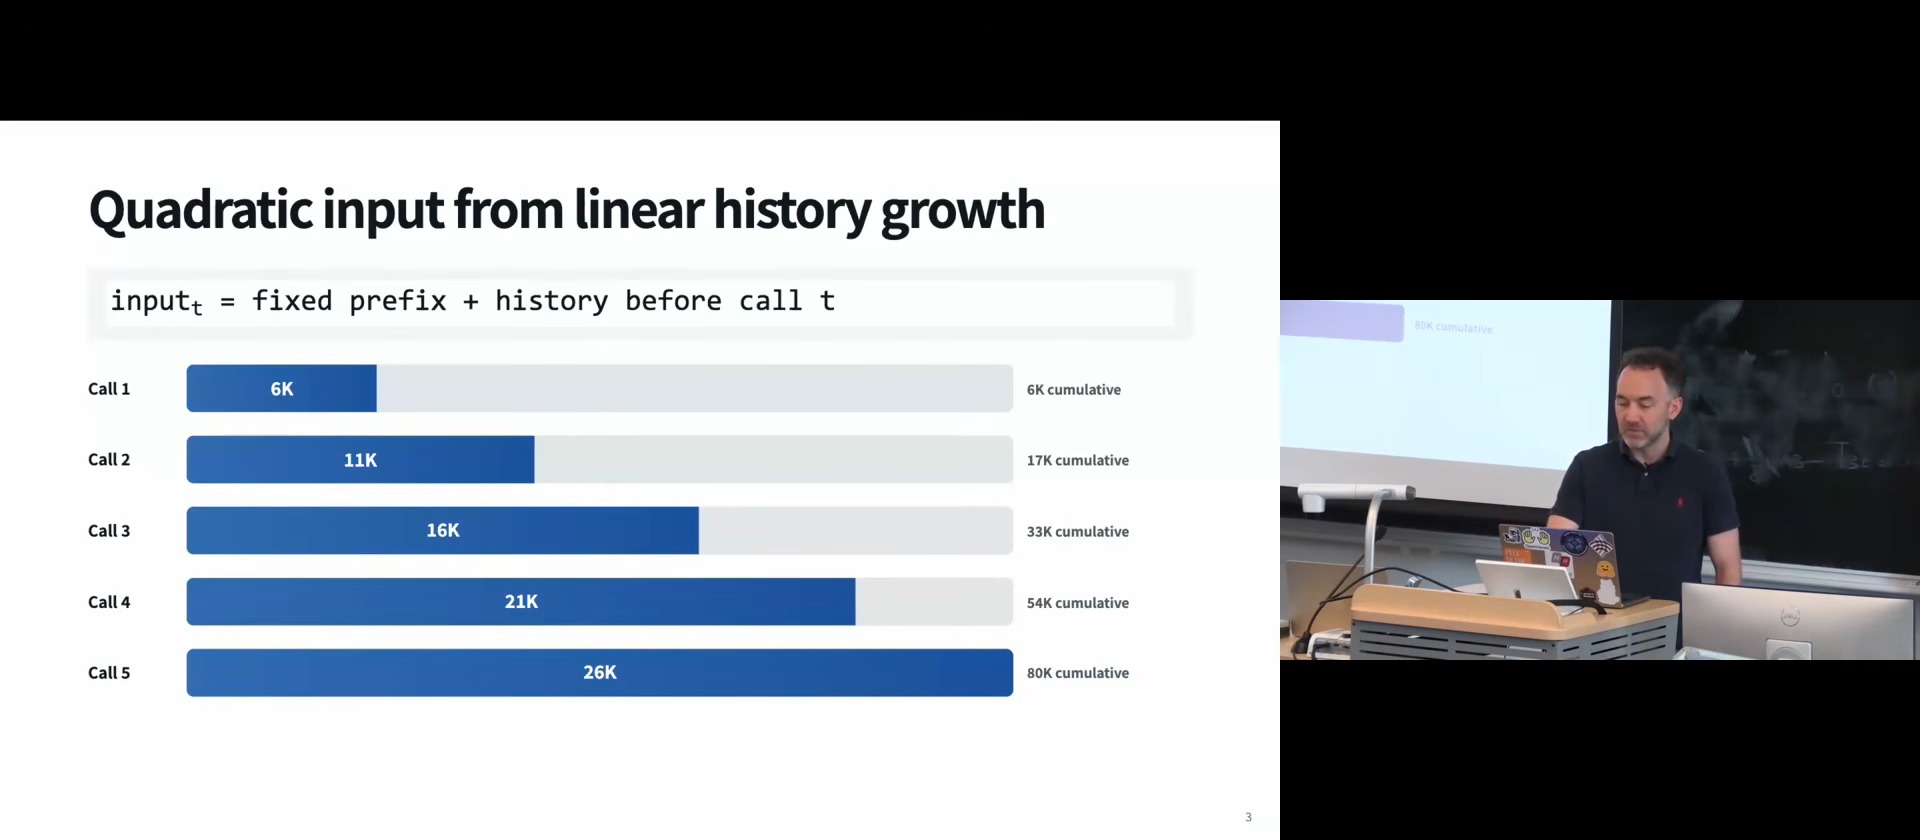
\includegraphics[width=\textwidth]{figures/fig_01_quadratic_growth.jpg}
\caption{线性历史、二次输入：每轮新增 6 到 26 个 token，五轮累计已经到 80\vtag}
\end{figure}
\srcnote{00:01:45--00:01:59}

这张图给出的工程结论是：能省下的计算不在“这一轮多算了什么”，而在“前面已经算过的部分能不能不重算”。如果把第 $t$ 轮之前的内容缓存下来、只处理新增的 $s$ 个 token，累计就从二次降为线性；本讲义第七、九节讲的 KV cache 与提示缓存，做的正是这件事。

\subsection{77,922 个 token 从哪里来}

讲者对自己团队的编码 agent OpenHands 做了统计：在 1,500 个会话上，平均每个会话消耗 77,922 个 token，而这些会话大多只是完成单个任务，并不是持续数天的长会话。构成如下（百分比前先写出绝对值范围的量级）：

\begin{itemize}
\item system prompt 与工具描述（约 15,000 到 18,000 token）：23\%；
\item 用户消息：9\%；
\item 模型的推理轨迹（reasoning）：9\%；
\item 模型直接回复：2\%；
\item 工具调用：20\%；
\item 工具结果：37\%。
\end{itemize}

\begin{figure}[H]
\centering
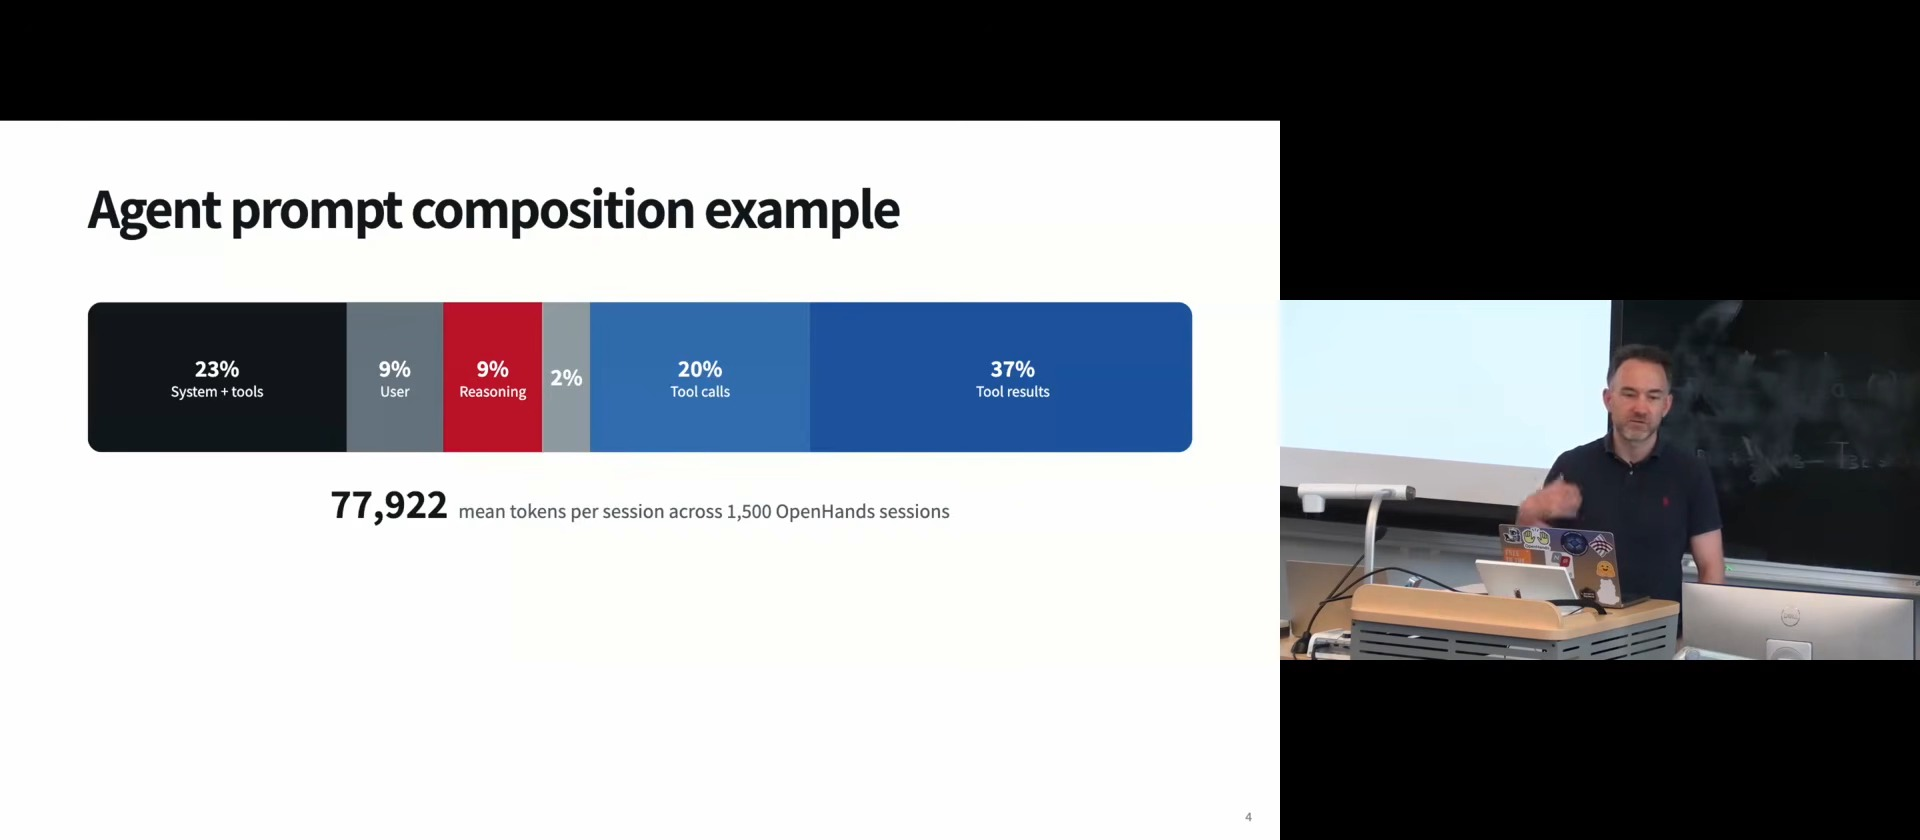
\includegraphics[width=\textwidth]{figures/fig_02_prompt_composition.jpg}
\caption{OpenHands 会话 token 构成：工具结果 37\%、system+tools 23\%、工具调用 20\%\vtag}
\end{figure}
\srcnote{00:02:45--00:02:59}

两件事值得单独记住。第一，固定前缀并不小：OpenHands 的 system prompt 约 15,000 到 18,000 token，随着接入工具数量变化，总前缀会在 8,000 到 20,000 token 之间浮动，这直接决定了“每一轮最小成本”。第二，动态部分的大头是工具结果，占 37\%，远高于模型对用户的直接回复 2\%；推理轨迹占 9\%，约为模型直接回复的五倍——token 主要花在“读环境”和“想”，而不是“说话”。用户消息只占 9\%，却往往包含最重要的约束，这一点在第九节讨论压缩时还会回来。

\begin{knowledgebox}{这讲为什么叫 “for agents”}
讲者一开始想把标题写成 “context management for long context LLMs”，因为这些技术大多是通用语言模型技术；他最终选择落在 agent 上，理由是长上下文在 agent 场景里的重要性被前置课程低估了：agent 的每一轮都在往上下文里追加指令、动作与观察，历史增长是任务的常态而不是例外。
\end{knowledgebox}

\subsection{两个必须同时解决的挑战}

幻灯片把长上下文的问题拆成两个正交的挑战。\textbf{容量（capacity）}问的是“模型能不能真正用上需要的那段证据”；\textbf{效率（efficiency）}问的是“服务系统能不能负担得起把它算出来并送出去”。前者靠架构、位置编码与训练数据塑造可用的上下文，并用评测来度量；后者靠注意力实现、KV 内存、缓存与压缩，改善成本与延迟。

\begin{figure}[H]
\centering
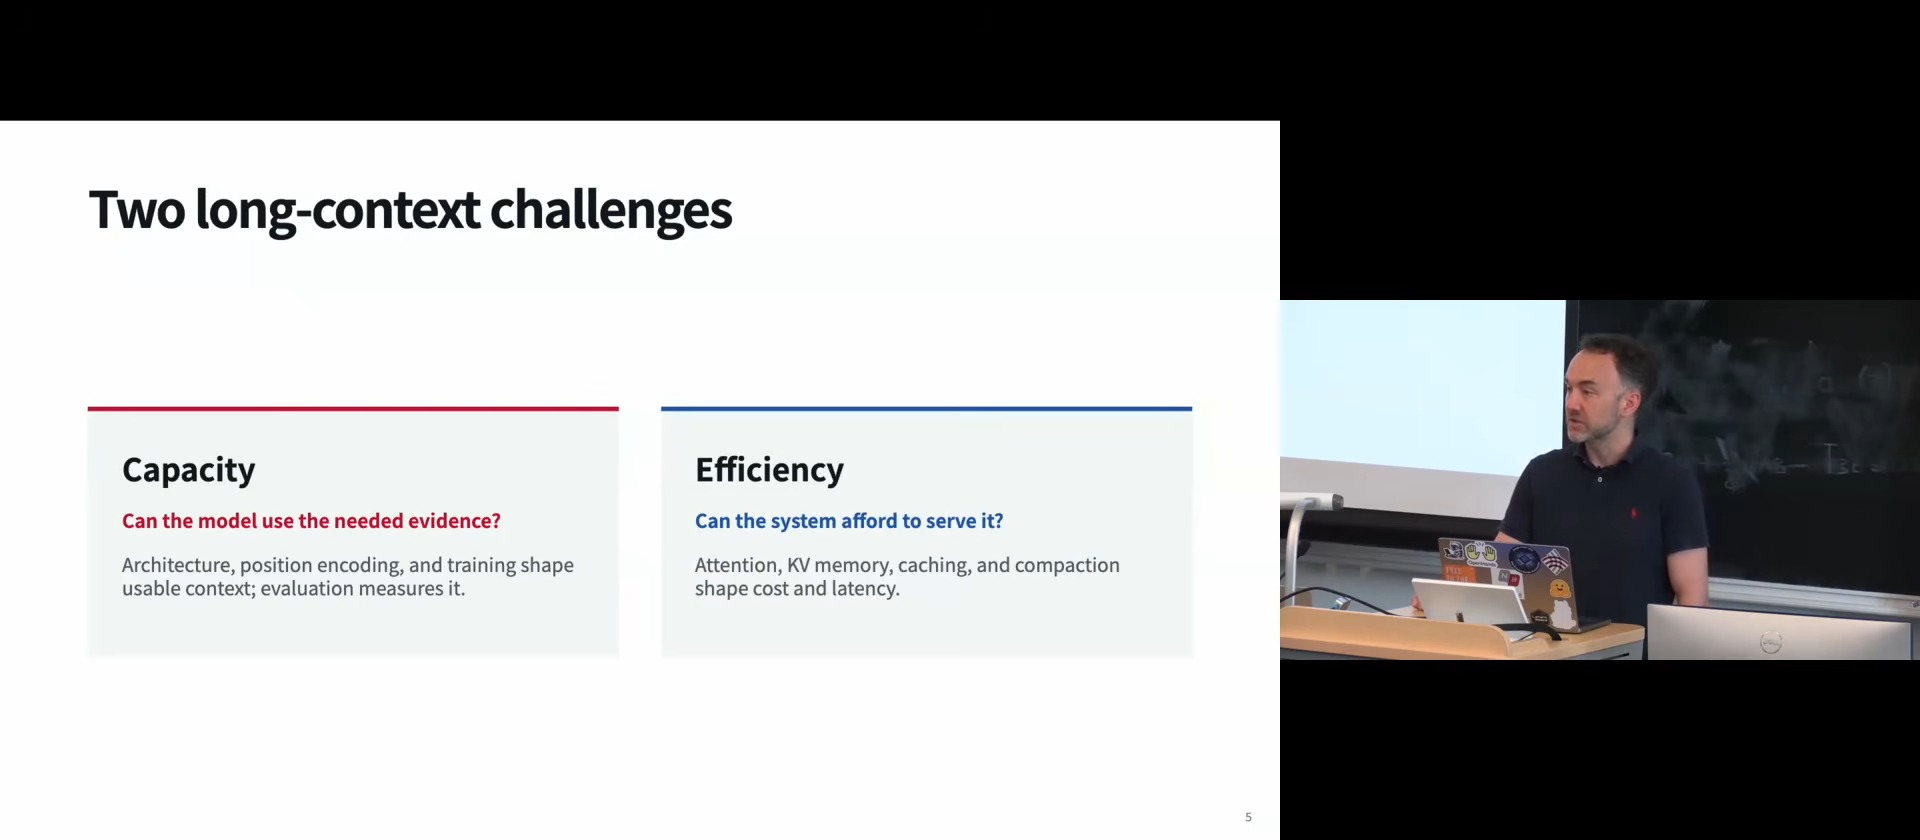
\includegraphics[width=\textwidth]{figures/fig_03_two_challenges.jpg}
\caption{两类挑战：capacity 对应“模型能否用上证据”，efficiency 对应“系统能否负担服务”\vtag}
\end{figure}
\srcnote{00:05:00--00:05:14}

\begin{importantbox}{容量与效率是两条独立的战线}
一个模型能接受 100 万 token 输入，不代表它能从中找回一个事实；一个系统能把成本压到十分之一，也不代表模型不会忘记中段的约束。判断长上下文方案时要把这两问分开问：谁负责让证据“可用”，谁负责让计算“可行”。本讲义第 3 节先看容量侧的失效证据，第 4 到 6 节看架构如何降低计算，第 7 到 9 节看缓存与压缩如何降低真实成本。
\end{importantbox}

\subsection{本章小结}
agent 的历史每轮线性增加，但每轮都要重读全部历史，累计计算按轮数平方增长；OpenHands 的真实会话平均已经要 77,922 个 token，其中工具结果与固定前缀占了大头。因此长上下文不是“把窗口开大”一个问题，而是容量与效率两条战线的配合。下一节进入服务系统的视角，先弄清 prefill、decode 与四个常用指标。

\section{推理服务：prefill、decode 与四个指标}

\subsection*{本节回答的问题}
一次请求在服务系统里经过哪些阶段？为什么“输入很长”和“输出很长”卡住的资源不一样？用来比较模型的 TTFT、TPOT、吞吐与成本分别测的是什么？

\subsection{服务栈的组成}

把模型放进产品里，请求会经过一条固定的流水线。\textbf{scheduler} 负责排队与组批（batching），决定哪些请求一起算；\textbf{prefill} 阶段一次处理 prompt 的全部位置，把每个 token 变成 KV；\textbf{decode} 阶段每步只生成一个新位置，并把这一步产生的 KV 追加进缓存；响应是流式返回的，缓存则是“读旧、写新”的持久状态。

\begin{figure}[H]
\centering
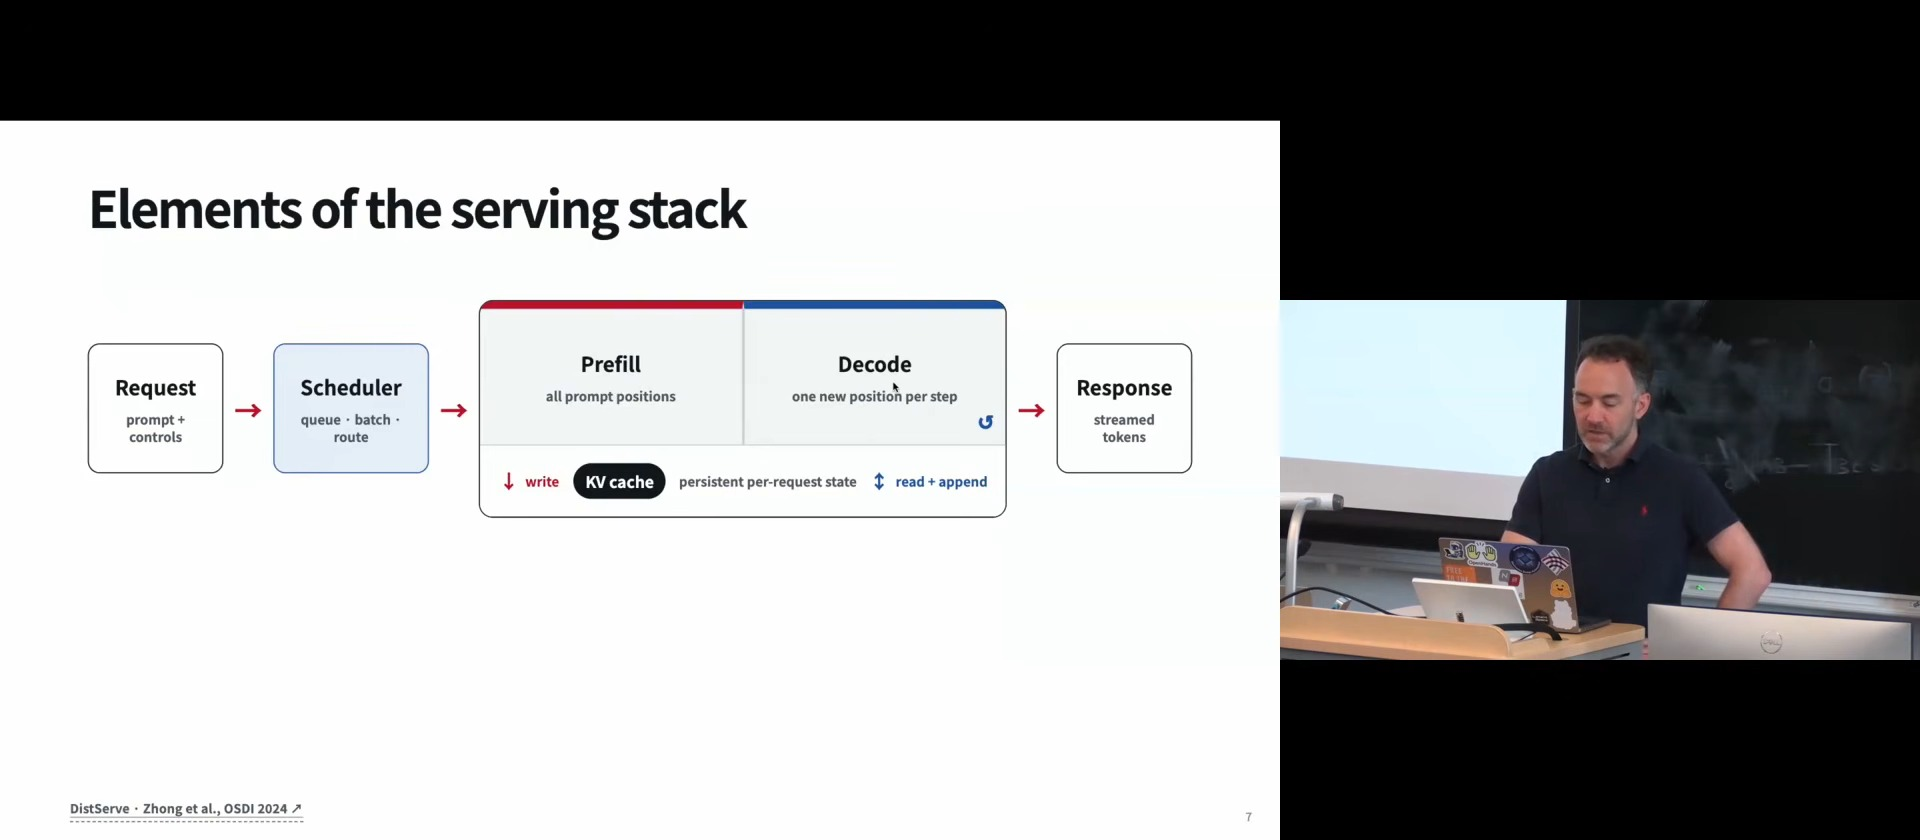
\includegraphics[width=\textwidth]{figures/fig_04_serving_stack.jpg}
\caption{服务栈：scheduler 组批，prefill 处理全部 prompt，decode 每步一个位置，KV cache 读写\vtag}
\end{figure}
\srcnote{00:06:15--00:06:29}

\subsection{prefill 与 decode 卡住的资源不同}

prefill 是“一次前向处理所有输入位置”，矩阵乘法的规模大、算术密度高，因此受算力限制，延迟随 prompt 长度增长；decode 每一步只处理一个位置，计算量很小，但要把整段序列的 KV 从显存里读出来，因此受显存带宽限制。讲者提醒：这个区别决定了优化手段——长输入先想到的是减少 prefill（缓存、压缩），长输出先想到的是提高每步的显存效率（批处理、KV 压缩）。

\begin{figure}[H]
\centering
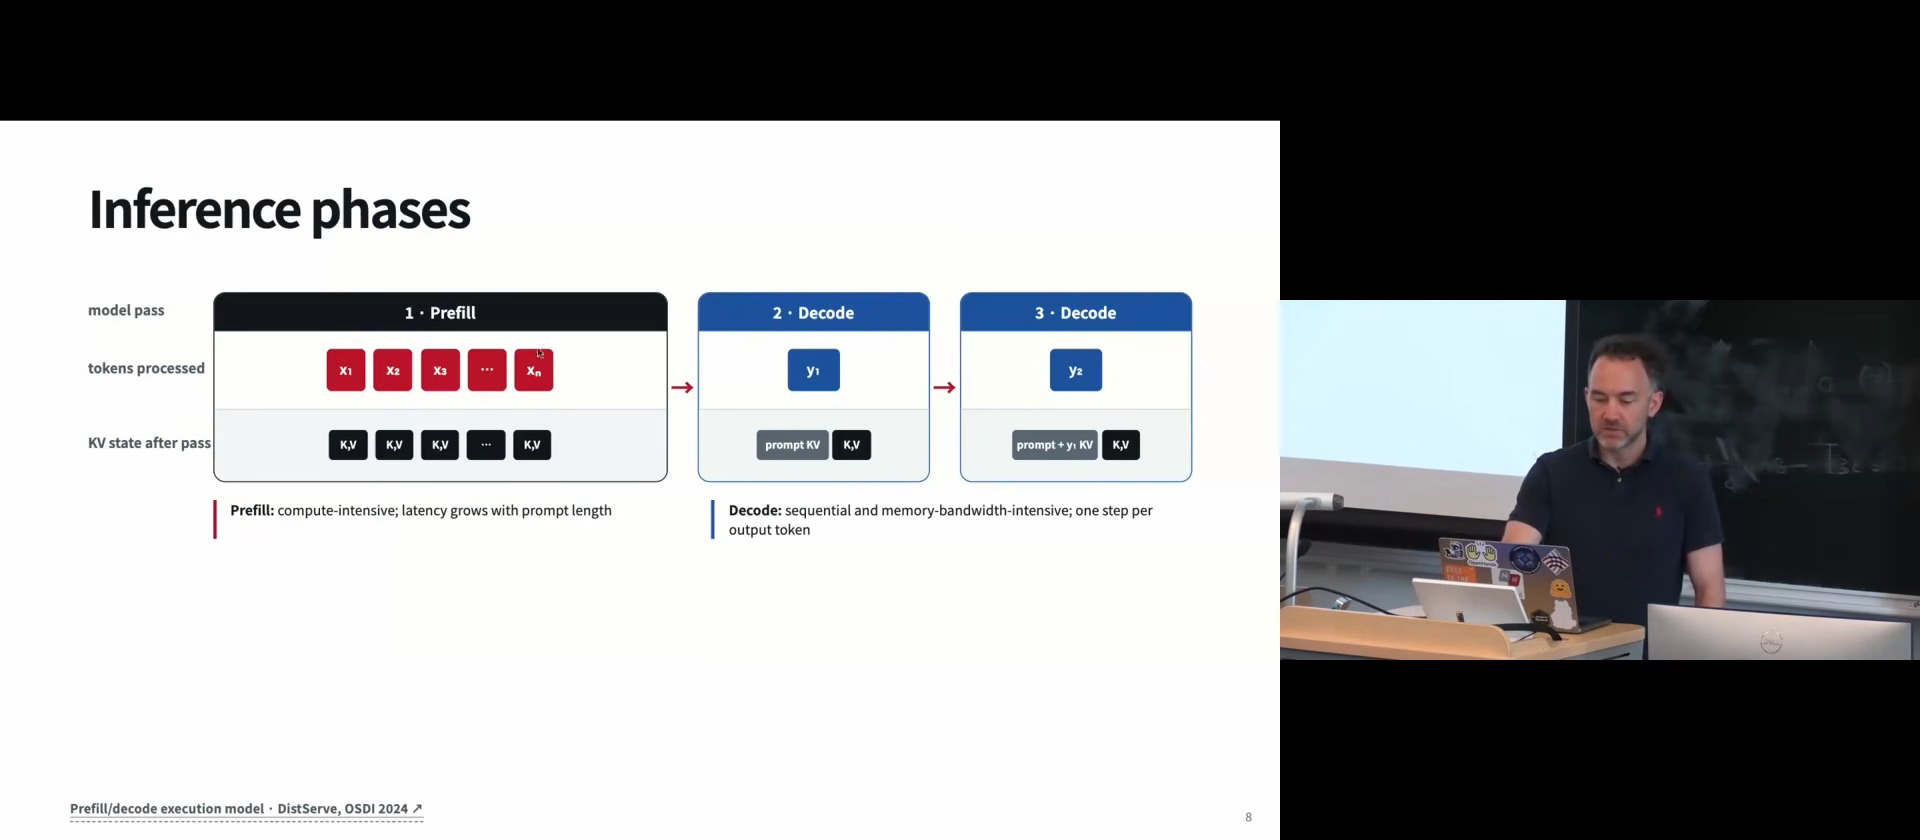
\includegraphics[width=\textwidth]{figures/fig_05_inference_phases.jpg}
\caption{两个推理阶段：prefill 计算密集且延迟随 prompt 增长，decode 顺序执行且受带宽限制\vtag}
\end{figure}
\srcnote{00:07:15--00:07:29}

\subsection{四项服务指标}

口语里说“这个模型很快”没有意义，服务侧用四个量描述体验与成本：

\begin{itemize}
\item \textbf{TTFT}（time to first token）：从请求到达至收到第一个输出 token 的时间，主要由 prefill 决定；
\item \textbf{TPOT}（time per output token）：输出 token 之间的平均间隔，主要由 decode 决定；
\item \textbf{throughput}（吞吐）：单位墙钟时间完成的 token 数或请求数，衡量整个系统而不只是单条请求；
\item \textbf{cost}（成本）：输入、缓存输入与输出三部分计费之和。
\end{itemize}

\[
\mathrm{TTFT}=t_{\text{first}}-t_{\text{arrive}},\qquad
\mathrm{TPOT}=\frac{t_{\text{last}}-t_{\text{first}}}{n_{\text{out}}-1}
\]

\begin{itemize}
\item $t_{\text{arrive}}$：请求到达服务系统的时刻；
\item $t_{\text{first}}$、$t_{\text{last}}$：第一个与最后一个输出 token 产生的时刻；
\item $n_{\text{out}}$：输出 token 数，分母减去 1 是把首 token 的等待排除在“间隔”之外。
\end{itemize}

\begin{figure}[H]
\centering
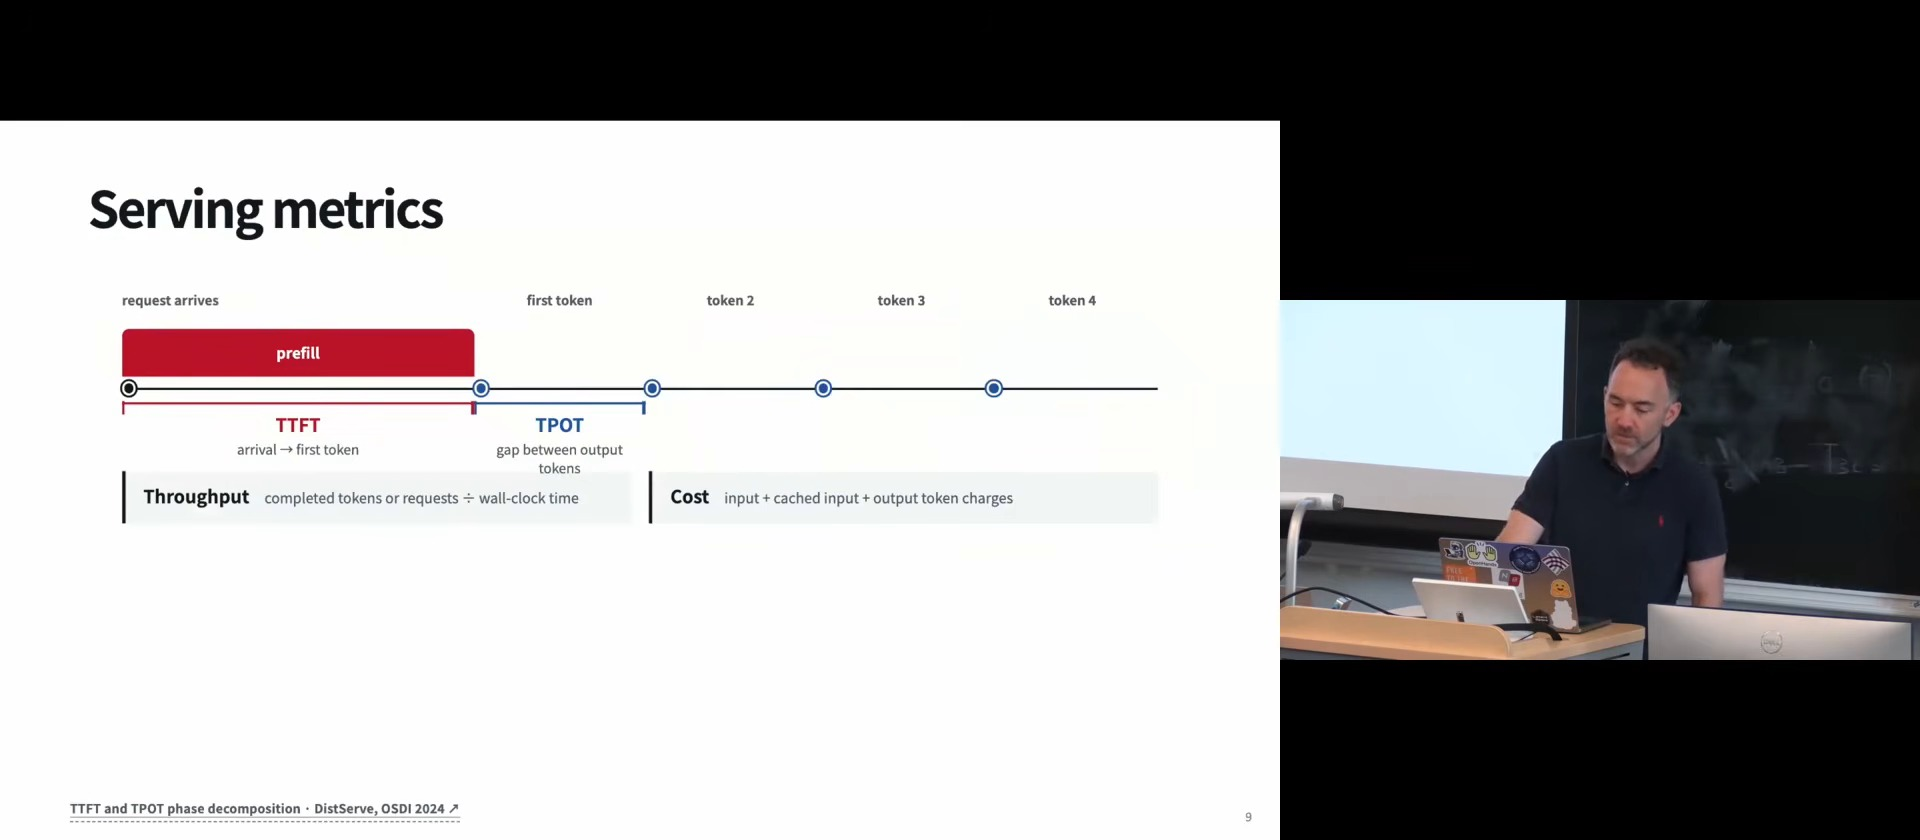
\includegraphics[width=\textwidth]{figures/fig_06_serving_metrics.jpg}
\caption{服务指标分解：TTFT 覆盖到达至首 token，TPOT 覆盖输出 token 间隔，另有吞吐与成本\vtag}
\end{figure}
\srcnote{00:07:45--00:07:59}

讲者强调这些指标之间存在取舍：交互式编码 agent 最在意 TTFT 与 TPOT，夜里跑批的后台 agent 可能完全不关心延迟，只在乎吞吐与成本。服务商通常也希望客户明确“更在乎哪一个”，以便针对性优化。

\subsection{同一个模型，不同供应商可以差两个数量级}

讲者用 OpenRouter 的公开数据说明这种差异：同一个 GLM 5.2，快的供应商大约每秒 63 个 token，另一家约 48，主流档位约 24，而最慢的一家只有大约每秒 3 个 token。对交互式 agent 来说，这直接决定“等待”还是“没法用”；对后台任务则主要影响成本与排队时间。

\begin{knowledgebox}{为什么同一模型会有不同速度}
供应商可能使用不同的量化精度、不同的投机解码配置、是否实现约束解码、不同的批处理与调度策略，服务稳定性也不一样。它们共享同一份权重，但整条服务栈的工程水平不同，所以 OpenRouter 的“模型页”要把 provider、价格、吞吐、TTFT 与缓存命中率分列——选模型其实是选“模型加供应商”的组合。
\end{knowledgebox}

\subsection{本章小结}
服务系统把请求拆成 prefill 与 decode：前者受算力限制、延迟随输入增长，后者受带宽限制、按步生成；TTFT 刻画等待、TPOT 刻画生成速度、吞吐刻画系统、成本刻画账单，四者取舍取决于交互还是后台。同一模型的供应商差异可以达到两个数量级，因此“用哪个模型”要连同“走哪家服务”一起决定。下一节回到模型内部，看注意力为什么天然昂贵，以及“能塞进窗口”与“真的能找回来”为什么是两件事。

\section{注意力的二次代价与“有效上下文”}

\subsection*{本节回答的问题}
标准注意力为什么是长上下文的瓶颈，代价到底有多大？为什么评测里一句简单的检索问题就足以暴露长上下文的失效？

\subsection{一次注意力前向做了什么}

自注意力先对输入做三个线性投影，得到查询、键与值，再用查询与键的相似度对值加权：

\[
Q=XW_Q,\quad K=XW_K,\quad V=XW_V,\qquad
A=\operatorname{softmax}\!\left(\frac{QK^{\top}}{\sqrt{d_k}}+M\right),\qquad
O=AV
\]

\begin{itemize}
\item $X\in\mathbb{R}^{n\times d}$：长度为 $n$ 的 token 状态矩阵，每一行是一个位置；
\item $W_Q,W_K,W_V$：把 $X$ 投影成查询、键、值的可学习矩阵；
\item $d_k$：单个注意力头的 key 宽度，除以 $\sqrt{d_k}$ 是为了稳定 logits 的尺度；
\item $M$：因果掩码，$M_{ij}=0$ 当 $j\le i$、否则为负无穷，保证每个位置只能看到自己与历史；
\item $A$：归一化后的注意力权重；$O$：加权求和后的输出。
\end{itemize}

\begin{figure}[H]
\centering
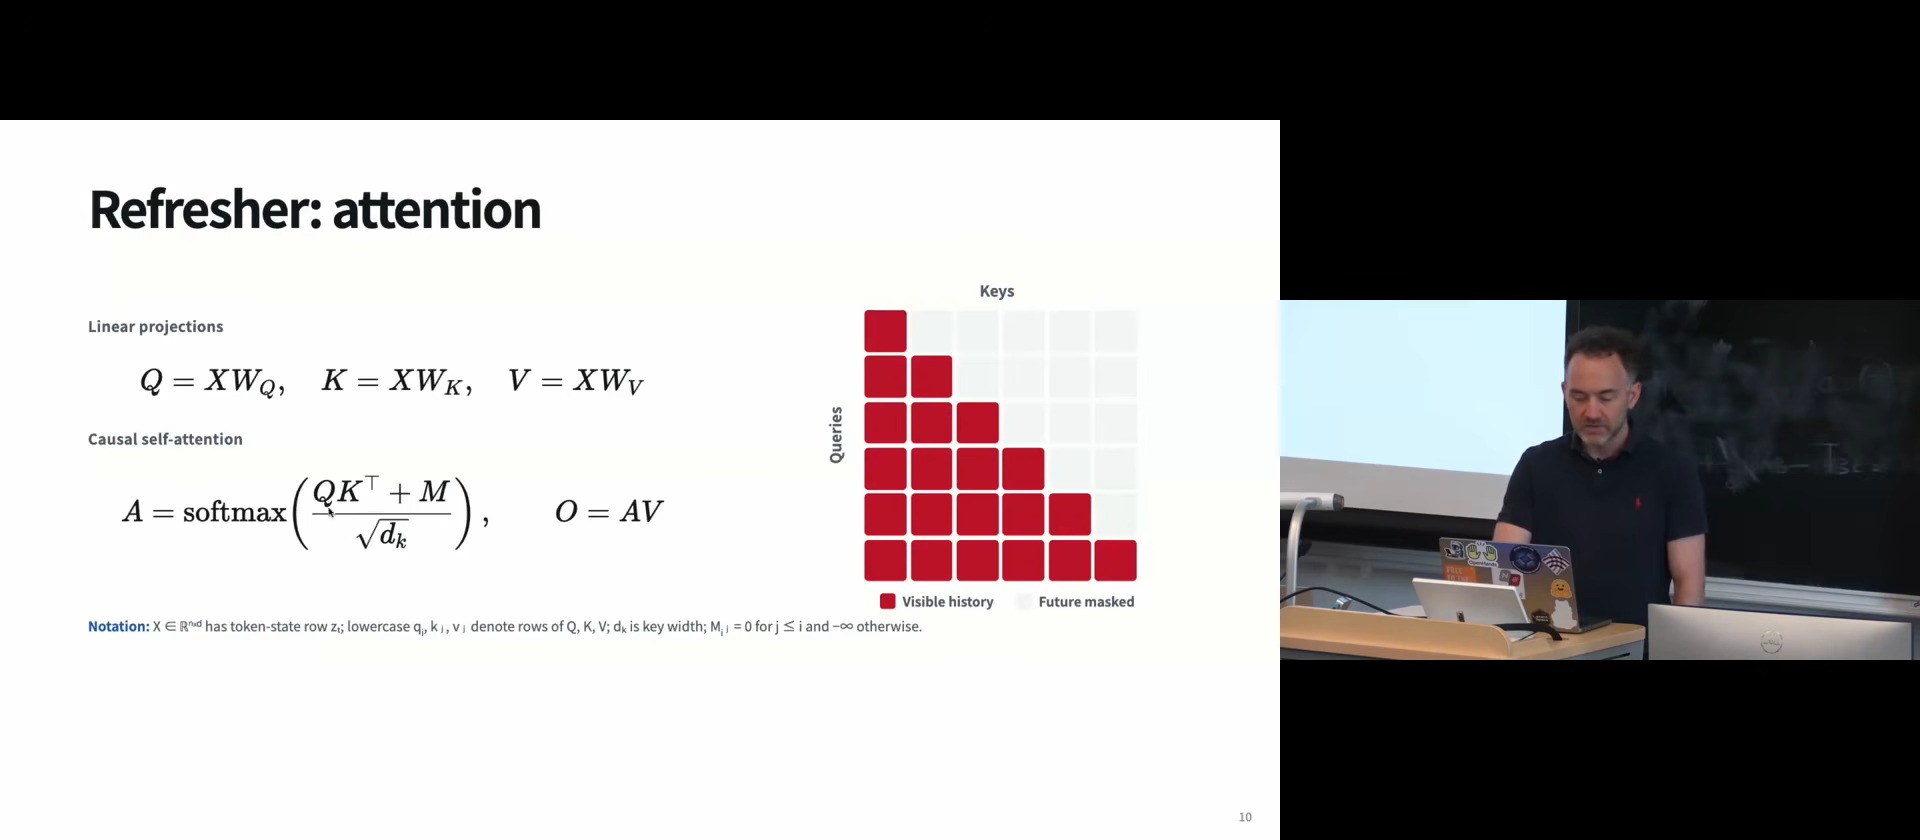
\includegraphics[width=\textwidth]{figures/fig_07_attention_refresher.jpg}
\caption{注意力复习：Q/K/V 线性投影、因果掩码、$A=\operatorname{softmax}(QK^{\top}/\sqrt{d_k})$ 与 $O=AV$\vtag}
\end{figure}
\srcnote{00:11:15--00:11:29}

键与值要为每个历史位置保留，这就是“注意力必须是全局的”的直接后果：查询要跟所有历史 key 比较，代价随序列长度平方增长。讲者现场算了一笔账：序列长度到 100 万时，成对比较约有

\[
N^2=10^{12}
\]

次；若把每次比较对应的向量内积也算进去，讲者给出的估算量级是 $10^{20}$ 次浮点运算。这两个数字解释了第 4 到 6 节为什么要把注意力换成局部、循环、稀疏或压缩的形式——它们都在回答“能否把成对比较的上限压成一个不随 $n$ 增长的常数”。

\subsection{广告上下文与有效上下文}

讲者用“大海捞针”（needle in a haystack）说明容量侧的失效：把一句事实（例如“旧金山最好吃的三明治店”）藏进一长串 Paul Graham 文章里，再问模型这个事实。随着上下文变长、以及事实被放在文档的不同深度，弱一些的模型准确率明显下滑。幻灯片上的热力图显示，GPT-4 的检索准确率在长上下文、且事实位于文档深度 10\% 到 50\% 附近时开始退化。

\begin{figure}[H]
\centering
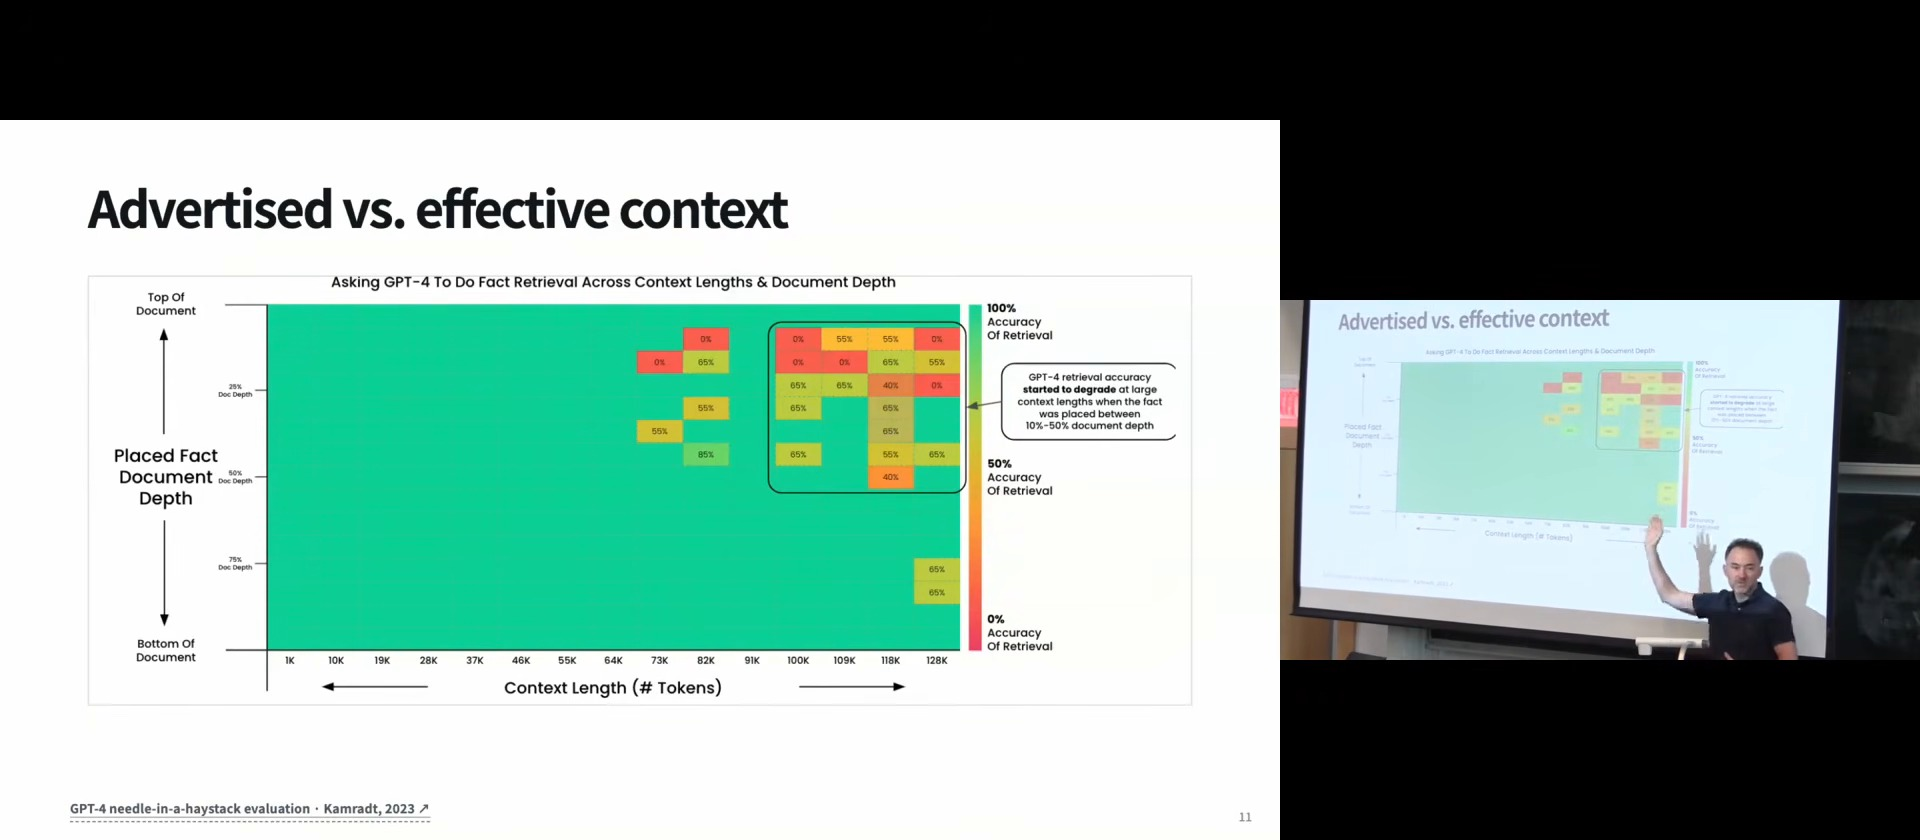
\includegraphics[width=\textwidth]{figures/fig_08_effective_context.jpg}
\caption{广告上下文与有效上下文：检索准确率随上下文长度和文档深度变化的热力图\vtag}
\end{figure}
\srcnote{00:13:00--00:13:14}

讲者提到 RULER 与 HELMET 是这一方向常用的评测集，并给出总结：上下文很长时，模型处理其中的信息可能变差。课堂上同学举出的真实失败是“忘记前面的上下文”，例如中途明确说了“不要删除这个文件”，模型后来还是把它删了——这类错误在交互式 agent 里代价很高，因为用户的增量指令往往夹在长历史中间。

\begin{warningbox}{能放进窗口 $\neq$ 能用上窗口}
把窗口从 128K 扩到 1M，改的是“物理容量”；检索准确率、指令跟随、跨段推理这些“有效容量”需要通过架构、位置编码、训练数据与评测共同保证。用长上下文方案时，不要用“窗口有多大”代替“任务成功率有多高”。
\end{warningbox}

\subsection{本章小结}
标准注意力让每个查询与全部历史成对比较，$n=10^6$ 时约 $10^{12}$ 次比较、算力估算到 $10^{20}$ 量级，这是效率侧的根问题；而“大海捞针”这类评测说明容量侧同样会失效，长窗口并不自动等于可用。接下来进入架构层：先看最直观的局部窗口与线性注意力，看它们各自如何把二次代价压下去，又付出了什么。

\section{架构层（一）：局部窗口、线性注意力与确定性更新}

\subsection*{本节回答的问题}
局部窗口、线性注意力与“键值状态矩阵”分别是怎么算的？它们把复杂度降到什么程度，代价是什么？

\subsection{局部建模：把比较数封顶}

几乎所有长上下文架构都从同一个动作出发：不再允许每个查询看全部历史，而是把“成对比较”的数量封一个常数上限。若每个查询只与窗口 $w$ 内的位置比较，成对比较代价从

\[
O(n^2)\ \longrightarrow\ O(wn)
\]

\begin{itemize}
\item $n$：序列长度；
\item $w$：局部窗口大小，也是每个查询保留的因果位置数；
\item 当 $w$ 是常数时，总工作量对 $n$ 是线性的。
\end{itemize}

\begin{figure}[H]
\centering
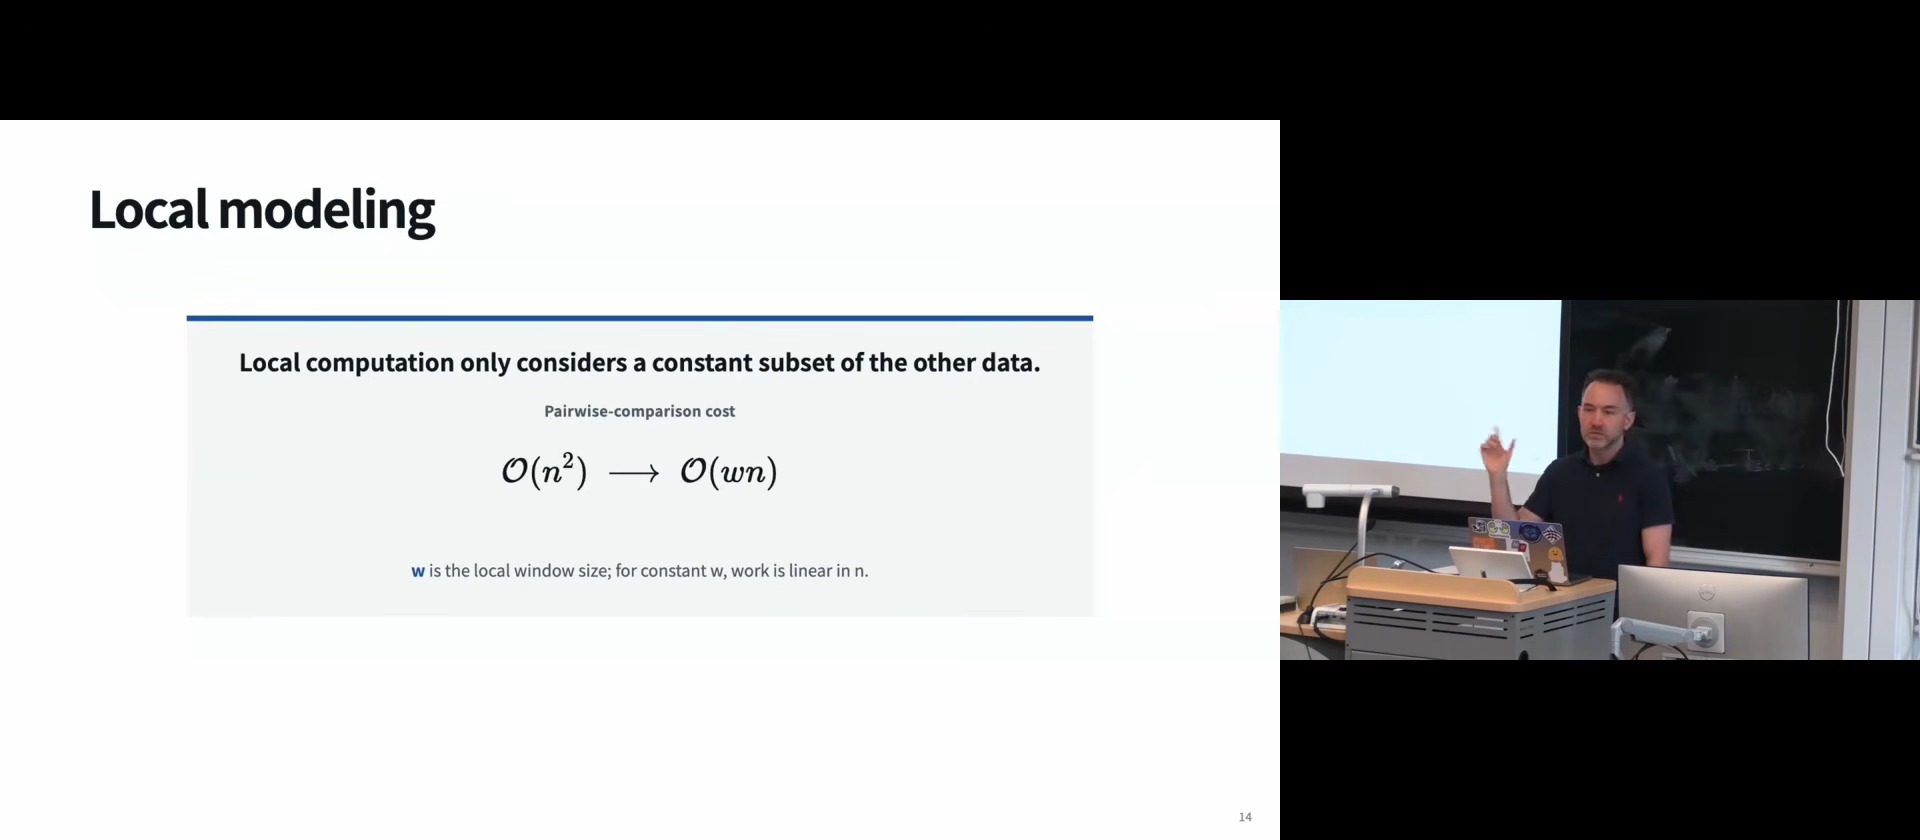
\includegraphics[width=\textwidth]{figures/fig_09_local_modeling.jpg}
\caption{局部建模：只与常数个子集比较，成对比较代价从 $O(n^2)$ 降到 $O(wn)$\vtag}
\end{figure}
\srcnote{00:16:30--00:16:44}

讲者把这类做法分成“局部”与“全局”两种角色：局部计算便宜但视野有限，全局计算可以跨整段序列传递信息但昂贵。今天主流的模型几乎都是混合体——多次局部计算之后再插入一次全局访问，然后重复。

幻灯片的架构表把六家模型的配比摆在一起。Qwen 与 GLM、Kimi 的局部对全局之比都约为 3:1，其中 Qwen 的局部用 Gated DeltaNet、全局用稀疏检索；Nemotron 是 4:1；Inkling 是 5:1；DeepSeek V4 则把窗口注意力与交错分支的稀疏结构拼在一起。

\clearpage
\begin{figure}[H]
\centering
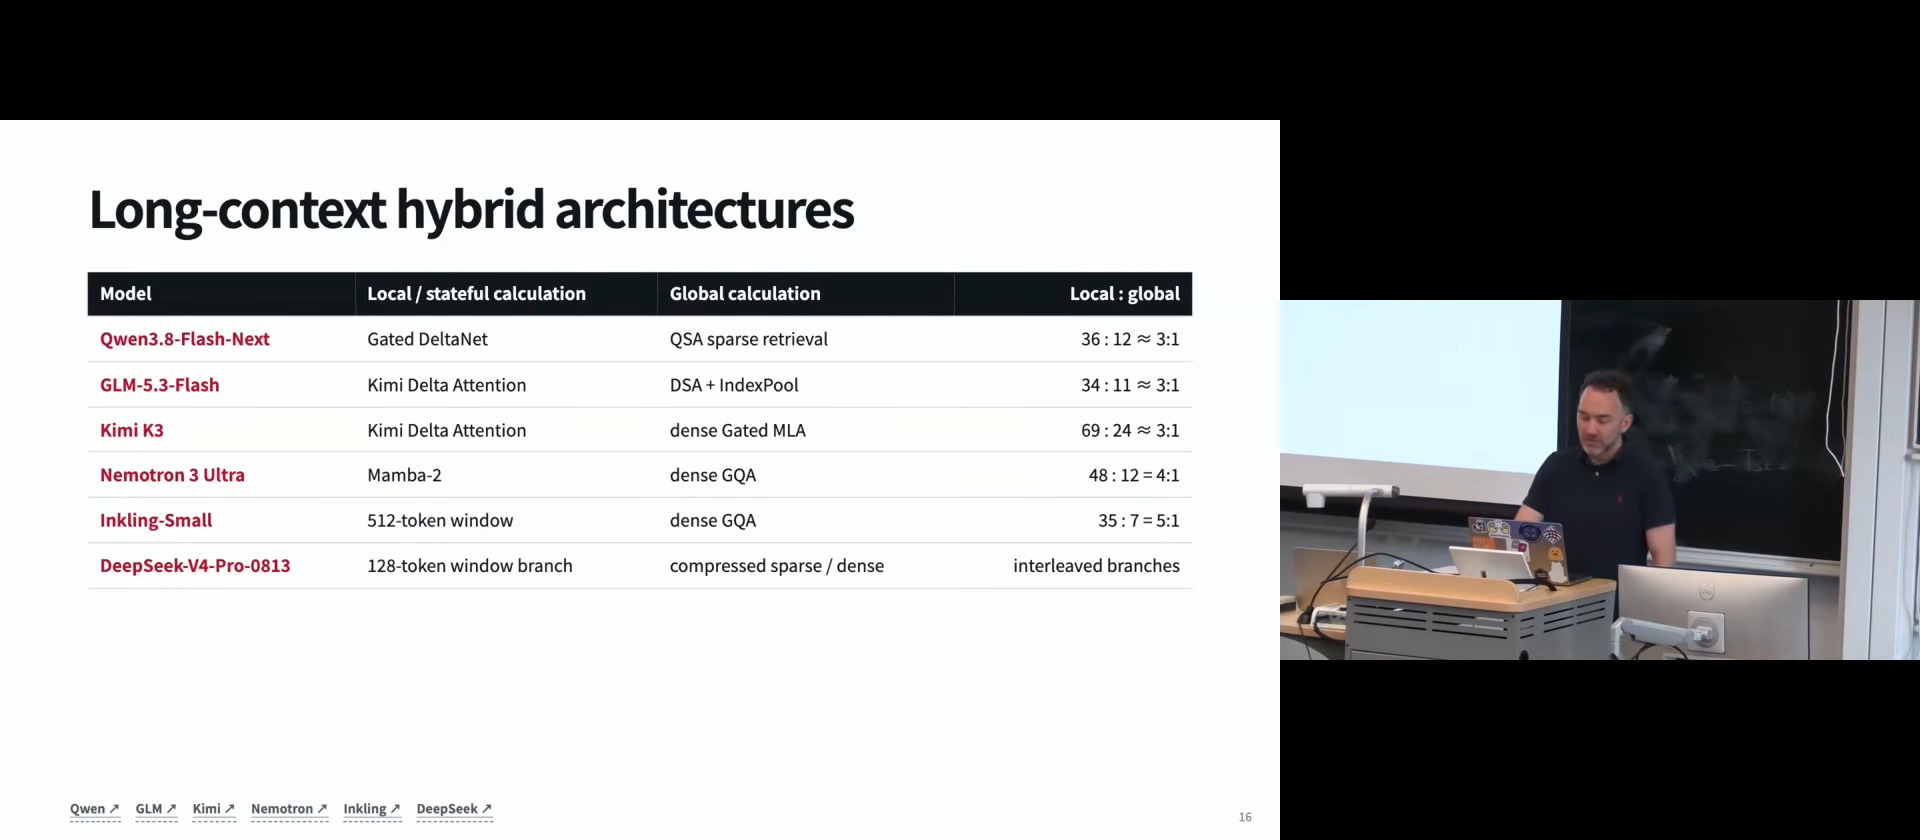
\includegraphics[width=0.86\textwidth]{figures/fig_10_hybrid_table.jpg}
\caption{长上下文混合架构表：局部机制与全局机制的配比集中在 3:1、4:1、5:1\vtag}
\end{figure}
\srcnote{00:18:30--00:18:44}

这张表的读法是先看“局部这一列”用了什么状态更新机制（Gated DeltaNet、Kimi Delta Attention、Mamba-2 等），再看“全局这一列”是稀疏检索、稀疏注意力还是稠密注意力，最后看比例。比例越高，说明模型越依赖便宜的局部状态、越少做昂贵的全局访问。

\subsection{滑动窗口注意力：最简单的局部实现}

滑动窗口注意力不改注意力的公式，只改可见集合：每个查询 只保留最近 $w$ 个因果位置，掩码写成 $0\le i-j<w$。工作量从 $O(n^2)$ 降到 $O(nw)$，实现代价极低。

\begin{figure}[H]
\centering
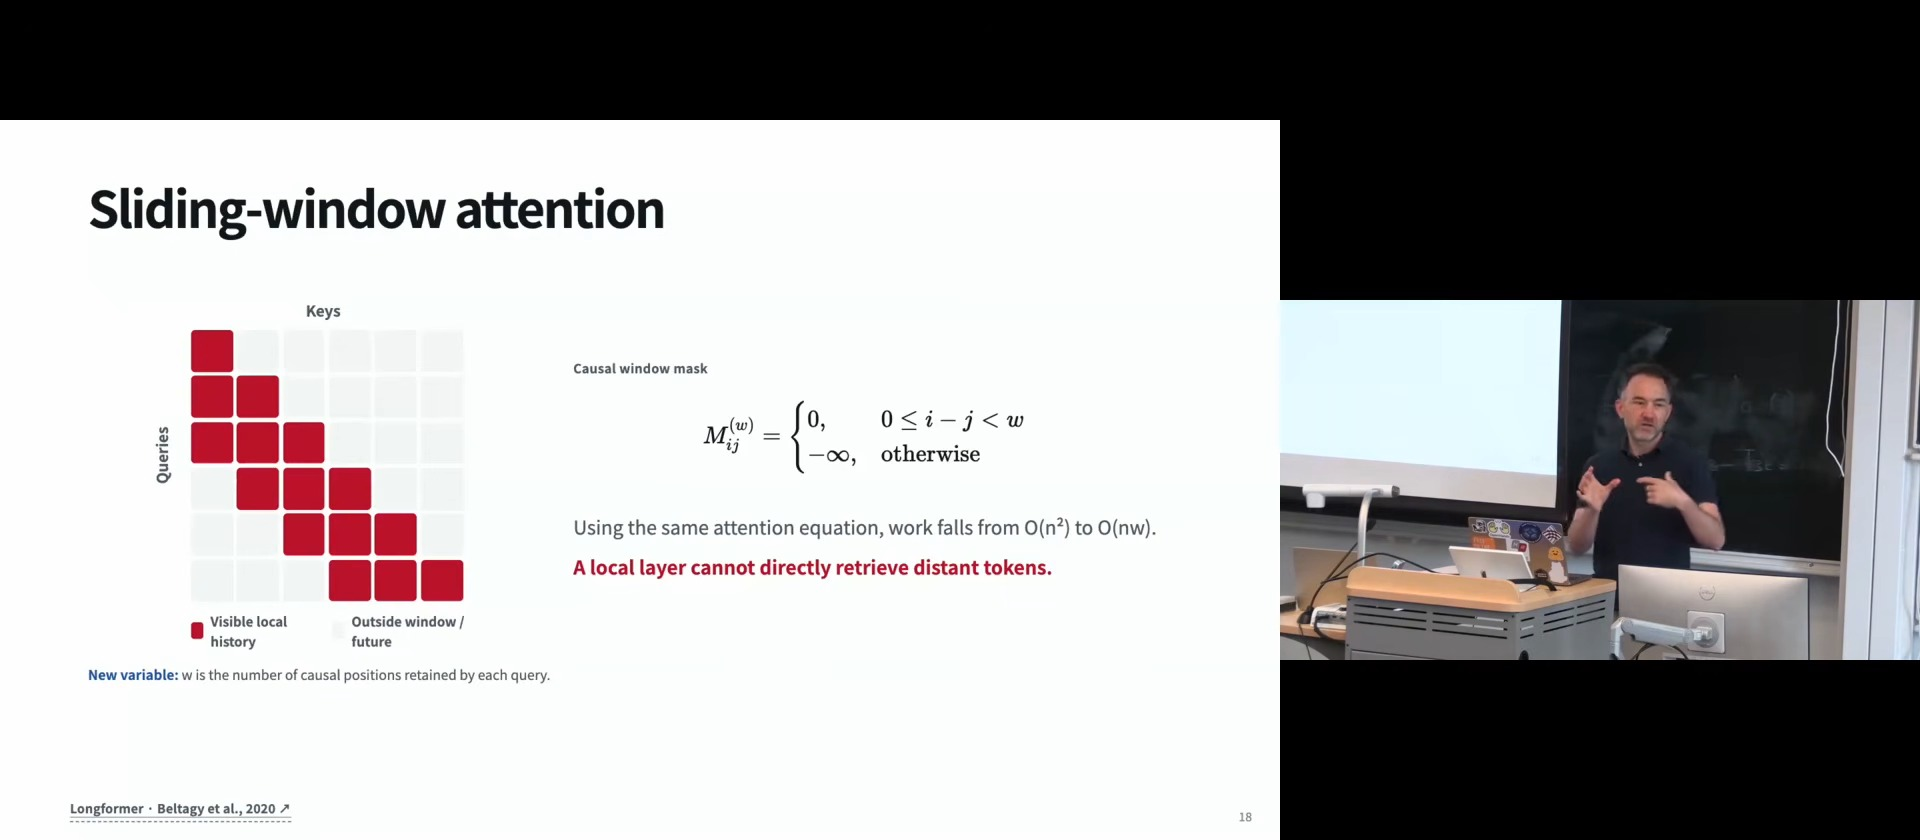
\includegraphics[width=\textwidth]{figures/fig_11_sliding_window.jpg}
\caption{滑动窗口注意力：因果窗口掩码 $0\le i-j<w$，窗口外的历史对局部层不可见\vtag}
\end{figure}
\srcnote{00:19:45--00:19:59}

滑动窗口的典型取值是 512 个 token：当前块的 512 个位置，加上前面若干块的 512 个位置，每个查询因此只与约 $w$ 个位置比较。

它有一个容易被忽略的性质：单层看不到远处，但多层堆叠后感受野会逐层扩大。第一层只能看到前一两块，第二层就能看到“前一块及其前一块”，于是形成渐渐扩张的窗口。讲者说这也是它被广泛采用的原因之一：改一行掩码，就得到一个跨层扩展的局部视野。代价同样明确——单个局部层无法直接检索远处的 token，需要靠混合架构中的全局层补上。

\subsection{线性注意力：去掉 softmax，换来可重结合的状态}

线性注意力的出发点是把注意力的归一化拿掉。标准注意力用 softmax 把相似度变成“和为一”的权重，从而可以只把注意力放在少数相关位置上；线性注意力改用双线性分数 $q^{\top}k_i$，牺牲了这种“相对比较”的能力，但换来一个关键性质：求和可以重新结合。把输出写出来就能看到：

\[
O_t=\sum_{i\le t}\left(q_t^{\top}k_i\right)v_i
      =q_t^{\top}\sum_{i\le t}k_i v_i^{\top}
      =q_t^{\top}S_t,
\qquad
S_t=S_{t-1}+k_t v_t^{\top}
\]

\begin{itemize}
\item $q_t,k_t,v_t$：第 $t$ 个位置的查询、键、值向量；
\item $S_t\in\mathbb{R}^{d_k\times d_v}$：把“键到值”的映射压成一个固定大小的状态矩阵，与序列长度无关；
\item 更新 $S_t=S_{t-1}+k_t v_t^{\top}$：每来一个新 token 只需一次外积加法，复杂度从 $O(n^2)$ 降到 $O(n)$，没有窗口项。
\end{itemize}

\begin{figure}[H]
\centering
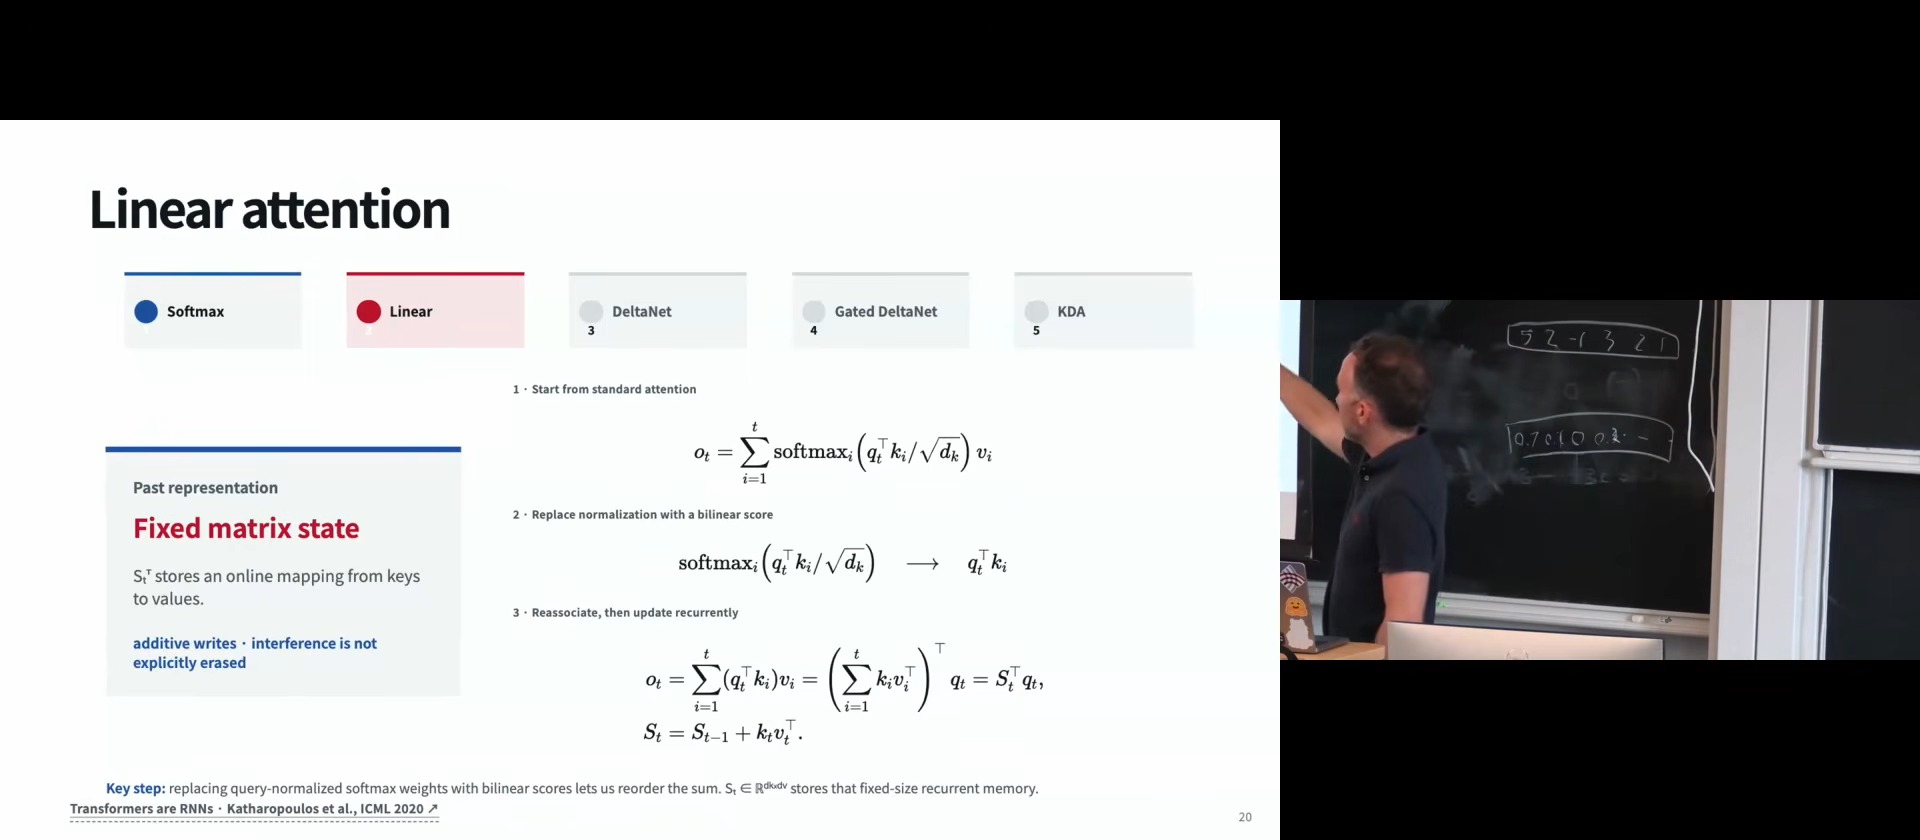
\includegraphics[width=\textwidth]{figures/fig_12_linear_attention.jpg}
\caption{线性注意力三步：去掉 softmax 归一化、改用双线性分数、重结合为固定状态 $S$\vtag}
\end{figure}
\srcnote{00:22:00--00:22:14}

讲者把它类比成循环网络：状态矩阵可以一直带着，每步常数时间更新。代价是表达力下降——没有了 softmax 的非线性，模型无法像注意力那样“只挑少数相关位置”，也就失去了对历史 token 做相对比较的能力。

\begin{warningbox}{线性注意力换到的是“固定预算”而不是“免费”} 
$O(n)$ 的代价是把所有历史压进一个固定大小的矩阵 $S$。当历史中存在大量相互冲突的信息时，加法写入会相互干扰，而且早期写入不会被显式擦除。后面的 DeltaNet 与门控机制，正是为了给这个状态加上“定向修正”和“遗忘”。
\end{warningbox}

\subsection{本章小结}
局部窗口把成对比较封顶到 $O(wn)$，滑动窗口是它最简单的实现且能跨层扩大感受野；线性注意力去掉 softmax，把键值历史压成固定大小的状态矩阵 $S_t$，用 $O(n)$ 的更新取代 $O(n^2)$ 的比较，代价是失去相对比较与显式擦除能力。主流模型因此采用“多次局部 + 少量全局”的混合结构，配比集中在 3:1 到 5:1。下一节看状态更新本身：DeltaNet 如何只写“预测误差”，门控与逐通道衰减又如何给状态加上遗忘。

\section{架构层（二）：DeltaNet、门控与逐通道遗忘}

\subsection*{本节回答的问题}
DeltaNet 与普通线性注意力的区别在哪一个词上？“门控”与“逐通道衰减”分别解决什么问题？

\subsection{DeltaNet：只写入预测误差}

线性注意力的更新是无条件的加法：不管状态里已经存了什么，都把 $k_t v_t^{\top}$ 加进去。DeltaNet 引入一个类似“误差修正”的动作。先用当前键去读状态里的预测值，再与真实值比较：

\[
\hat{v}_t=S_{t-1}^{\top}k_t,\qquad
e_t=v_t-\hat{v}_t,\qquad
S_t=S_{t-1}+\beta_t\,k_t e_t^{\top}
\]

\begin{itemize}
\item $\hat{v}_t$：用上一步状态读出的预测值；
\item $e_t$：预测误差，即“真实值减去预测值”；
\item $\beta_t\in[0,1]$：修正强度，作用类似学习率，越小更新越保守；
\item $S_t$：修正后的状态。注意更新方向沿 $k_t$，与 $k_t$ 无关的记忆不会被这次写入覆盖。
\end{itemize}

\begin{figure}[H]
\centering
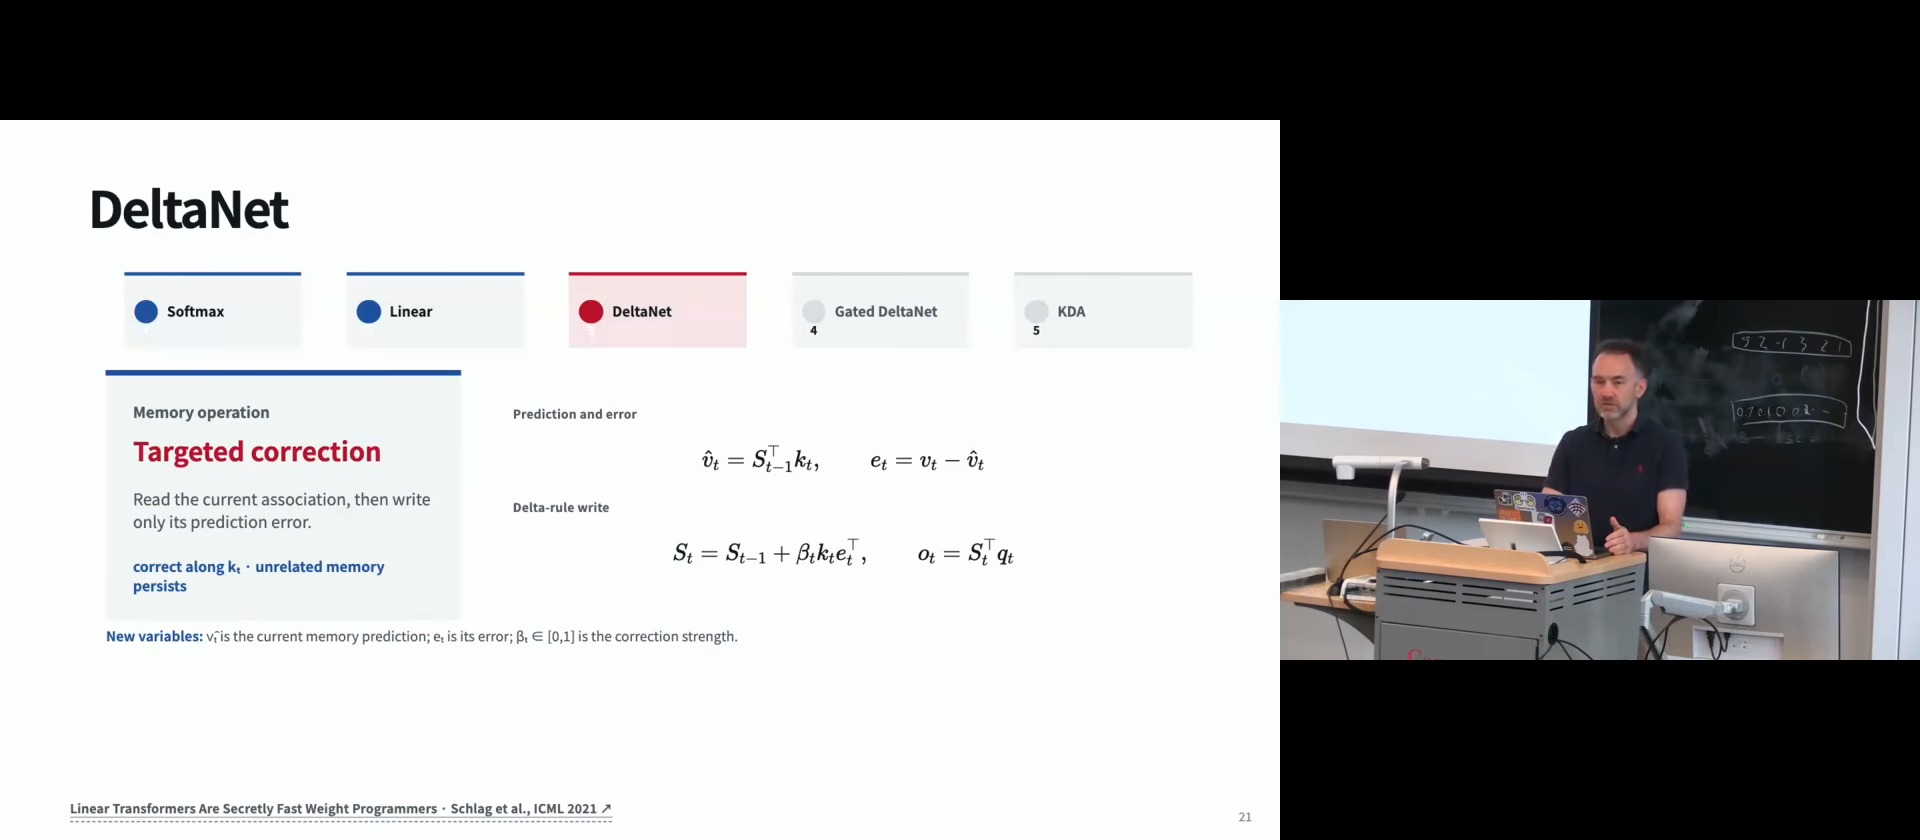
\includegraphics[width=\textwidth]{figures/fig_13_deltanet.jpg}
\caption{DeltaNet：先读出预测 $\hat{v}_t=S_{t-1}^{\top}k_t$，再只写入误差 $e_t=v_t-\hat{v}_t$\vtag}
\end{figure}
\srcnote{00:27:45--00:27:59}

讲者解释直觉：这一步把状态往“让当前键映射到正确值”的方向推，同时又不会大幅改动与当前键无关的记忆。与线性注意力相比，它多了一个“先读后写”的闭环，因此历史冲突时状态不会简单叠加，而是被定向修正。

\subsection{门控：先遗忘，再修正}

DeltaNet 的问题在于它缺少遗忘机制：很久以前一个“奇怪的键”仍然可能对现在的预测产生很大影响。解决办法是在写入前先把整个状态衰减一次：

\[
\tilde{S}_{t-1}=\alpha_t S_{t-1},\qquad
S_t=\tilde{S}_{t-1}+\beta_t k_t\left(v_t-\tilde{S}_{t-1}^{\top}k_t\right)^{\top}
\]

\begin{itemize}
\item $\alpha_t\in[0,1]$：标量保留门（retention gate），越小表示遗忘越快；
\item $\tilde{S}_{t-1}$：衰减后的状态；
\item $\beta_t$：照旧是定向修正的强度。取 $\alpha_t=1$ 就退化为 DeltaNet。
\end{itemize}

\begin{figure}[H]
\centering
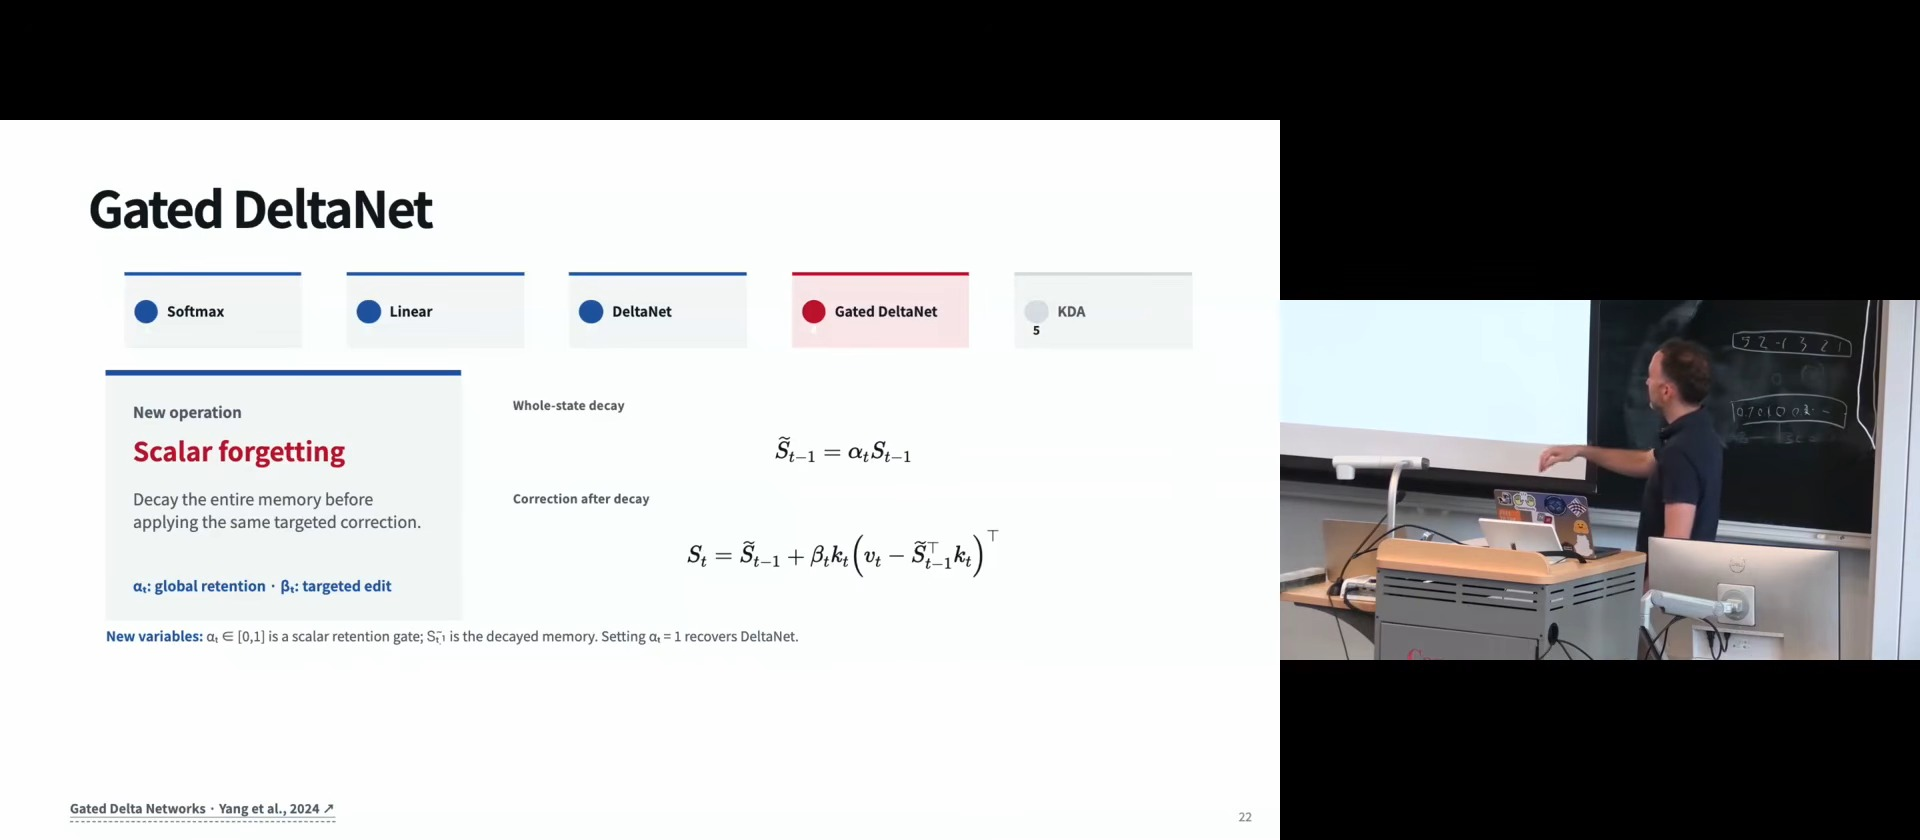
\includegraphics[width=\textwidth]{figures/fig_14_gated_delta.jpg}
\caption{Gated DeltaNet：先把整个状态乘 $\alpha_t$ 衰减，再做同一次定向修正\vtag}
\end{figure}
\srcnote{00:28:45--00:28:59}

讲者把两个门的分工总结成一句话：$\alpha_t$ 管“全局保留”，$\beta_t$ 管“定向编辑”。调小 $\alpha_t$ 会让模型更局部，调大则让信息保留更久——这给了训练一个连续可调的“记忆长度”旋钮。

\subsection{逐通道衰减：每个特征有自己的寿命}

标量门控仍是“整个状态一起衰减”，但不同的 key 维度可能有多长多短的记忆需求。Kimi Delta Attention（KDA）把标量换成向量，让每个通道独立衰减：

\[
D_t=\operatorname{Diag}(\alpha_t),\qquad
S_t=\left(I-\beta_t k_t k_t^{\top}\right)D_t S_{t-1}+\beta_t k_t v_t^{\top}
\]

\begin{itemize}
\item $\alpha_t\in[0,1]^{d_k}$：逐通道保留门；$D_t$ 是它的对角矩阵；
\item $I$：$d_k\times d_k$ 单位阵；$k_t k_t^{\top}$ 是沿当前键方向的投影；
\item 当所有通道的保留值相同时，KDA 退化为 Gated DeltaNet。
\end{itemize}

\begin{figure}[H]
\centering
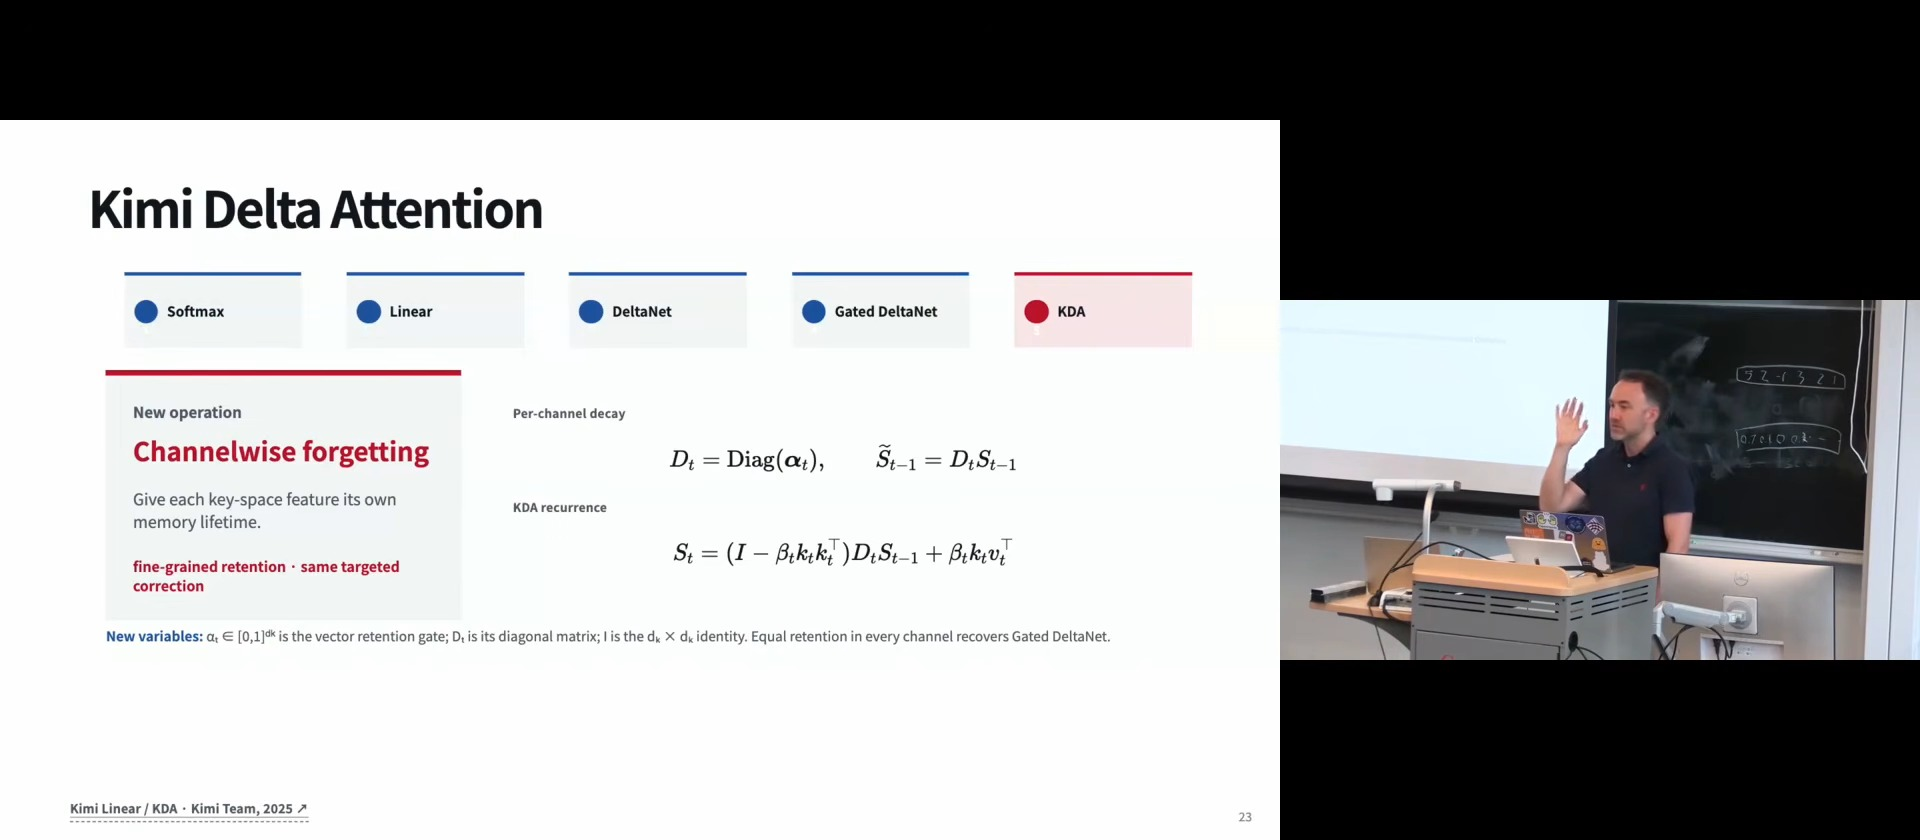
\includegraphics[width=\textwidth]{figures/fig_15_kda.jpg}
\caption{Kimi Delta Attention：逐通道衰减 $D_t=\operatorname{Diag}(\alpha_t)$，每个 key 维度有独立寿命\vtag}
\end{figure}
\srcnote{00:30:15--00:30:29}

逐通道衰减的意义是：同一段历史里，某些特征可以长期保留，另一些可以快速遗忘，模型不必用一个统一的遗忘速度兼顾两种需求。讲者说多数这类方法“深入数学看都在试图更好地预测注意力的输出”，这里只需记住机制层面的差异——加法写入、误差修正、整体衰减、逐通道衰减，是四个递进的层次。

\begin{importantbox}{四个更新层次的记忆口诀}
线性注意力是“加”；DeltaNet 是“先读再改，只写误差”；Gated DeltaNet 是“先衰减整块，再改误差”；KDA 是“每个通道各自衰减，再改误差”。越往后表达力越强，代价是核函数与并行实现越复杂——这一点在第七节会以“没有现成 kernel”的形式变成工程问题。
\end{importantbox}

\subsection{本章小结}
DeltaNet 用“读出预测、只写误差”把线性注意力的加法写入变成定向修正，门控 $\alpha_t$ 在修正前给状态一次整体遗忘，KDA 再把标量遗忘细化到每个通道。至此局部状态的三层机制（局部窗口、线性状态、门控修正）讲完，下一节转到全局侧：稀疏注意力如何在便宜的前提下取回远处的信息，以及 KV 压缩如何缩减必须保存的键值。
\section{架构层（三）：稀疏注意力与 KV 压缩}

\subsection*{本节回答的问题}
“只保留一部分历史”有哪两种做法，各自的失败模式是什么？如果不删历史，能不能把要保存的键值本身压缩变小？

\subsection{固定模式与内容相关：两种稀疏}

稀疏注意力不改变“要比较”这件事，只限制比较的对象。幻灯片把它分成两族。第一族是\textbf{固定模式}：可见集合由位置决定，例如“窗口内 $0\le i-j<w$ 加上一组固定的全局位置 $G$”。

\[
S_{\text{fix}}=\{(i,j):j\le i,\ i-j<w\}\ \cup\ \{(i,g):g\in G\}
\]

\begin{itemize}
\item $S_{\text{fix}}$：第 $i$ 个查询允许看到的键的下标集合；
\item $w$：局部窗口；$G$：一组固定的全局位置；
\item 成本可预测、与输入无关，但模式不能随查询变化，可能恰好错过需要的那一段。
\end{itemize}

第二族是\textbf{内容相关}：先用一个便宜的打分函数（例如把查询与键下投影到很小的维度）算出每个键的分数，只保留最高的若干个，再在这个集合上做完整注意力。

\[
S_{\text{dyn}}=\operatorname{TopK}_j\ s(q_i,k_j)
\]

\begin{itemize}
\item $s(\cdot,\cdot)$：廉价的相关性打分，可以是低维点积；
\item $S_{\text{dyn}}$：随查询变化而变化的保留集合；
\item 优点是可以自适应检索；风险是选择器一旦挑错，真正相关的键就被永久排除在这一次注意力之外。
\end{itemize}

两族都在各自的保留集合上重新归一化，因此输出的权重仍然和为一。

\begin{figure}[H]
\centering
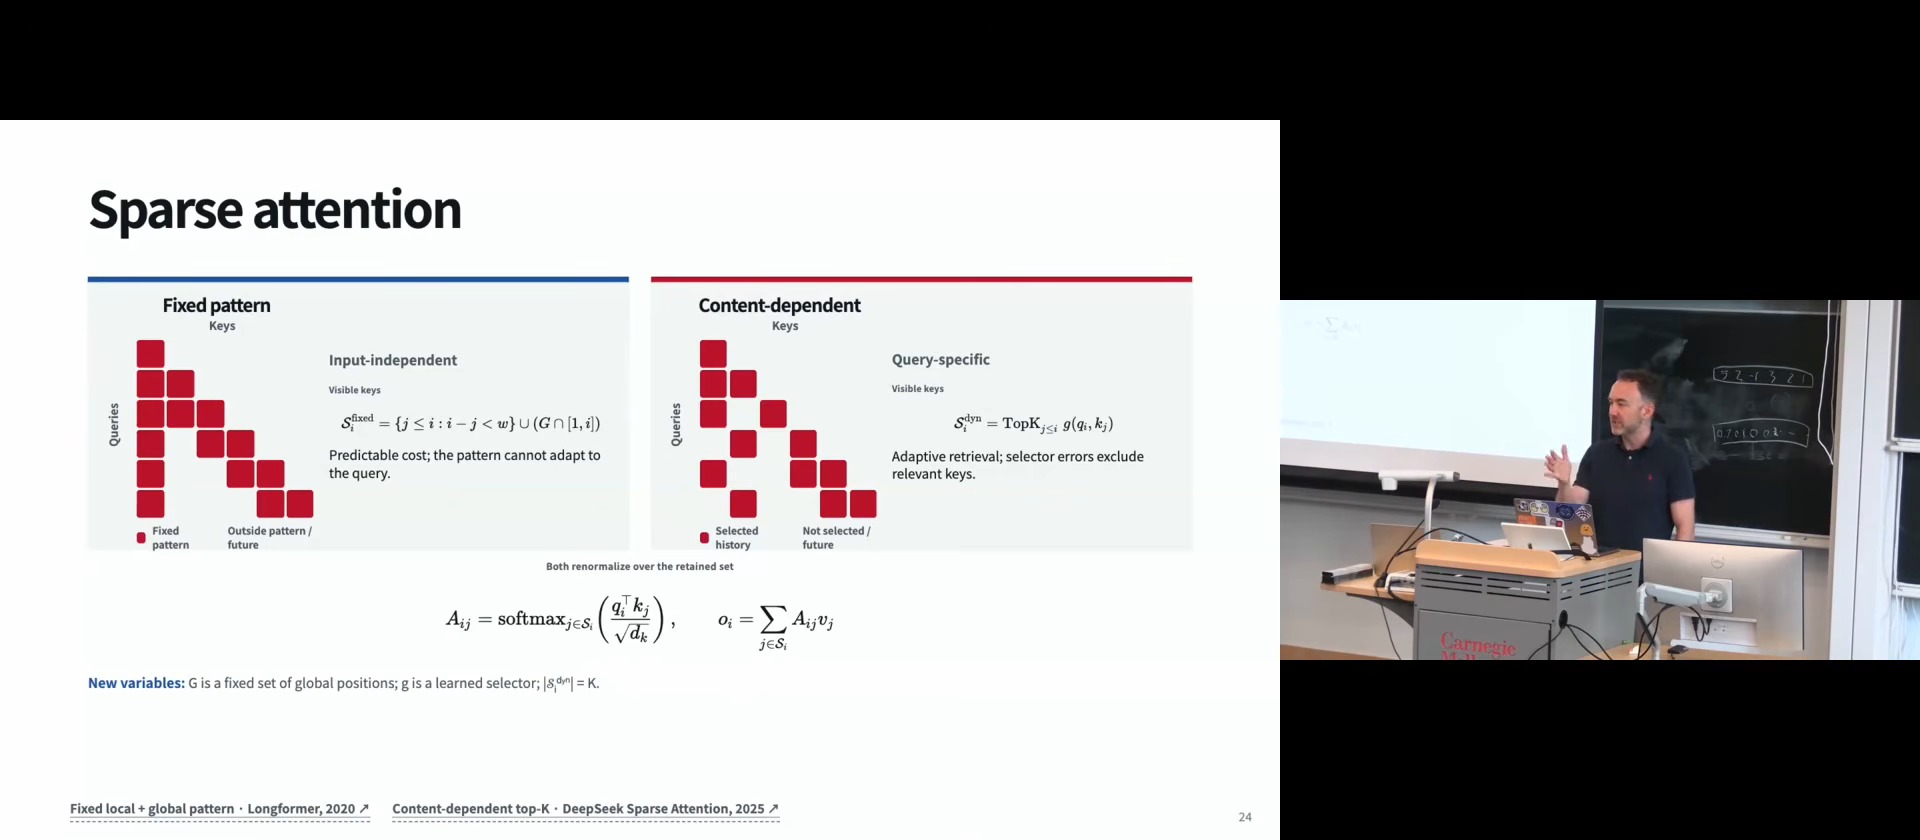
\includegraphics[width=\textwidth]{figures/fig_16_sparse_attention.jpg}
\caption{稀疏注意力两族：固定模式 $S_{\text{fix}}$ 依赖位置，内容相关 $S_{\text{dyn}}$ 用 TopK 选键\vtag}
\end{figure}
\srcnote{00:31:45--00:31:59}

讲者补充了实现侧的区别：固定模式（以及滑动窗口这类规则结构）很容易写成高效 kernel，一般只需一遍计算；内容相关需要先算一次低维打分、选出 TopK、再做一次完整注意力，通常是两遍，但精度上限更高。课堂上有人问 TopK 用什么相似度，讲者回答通常是点积而不是余弦距离，也不确定是否提前做了归一化。

\begin{warningbox}{稀疏的失效发生在“选择器”上}
固定模式的失败是“模式没有覆盖”，内容相关的失败是“打分选错了”。后者更隐蔽：模型看起来有全局访问能力，实际每一次都只看到被选择器筛过的片段。评测长上下文模型时，除了看它能否回答，还要看回答是否依赖某个本可被选中的远处证据。
\end{warningbox}

\subsection{KV 压缩：不删历史，改存更小的东西}

稀疏注意力减少“看多少”，KV 压缩减少“存多少”。标准多头注意力（MHA）为每个头保存独立的键与值；分组查询注意力（GQA）让多个查询头共享一组键值头，把 KV 头数降到 $h$ 的四分之一或八分之一；多查询注意力（MQA）是极端情形，所有查询头共享一组键值；多头潜在注意力（MLA）不减少头数，而是先把键值投影到一个压缩的 latent，再按头重建。

\[
\text{KV bytes}=2\cdot L\cdot n_{\text{kv}}\cdot d_h\cdot n_{\text{ctx}}\cdot b
\]

\begin{itemize}
\item $L$：层数；$n_{\text{kv}}$：键值头数；$d_h$：每头维度；$n_{\text{ctx}}$：上下文长度；
\item $b$：每个元素占的字节数；系数 2 表示键与值各存一份；
\item GQA/MQA 缩小 $n_{\text{kv}}$，MLA 缩小实际缓存的 $d_h\cdot n_{\text{kv}}$。
\end{itemize}

\begin{figure}[H]
\centering
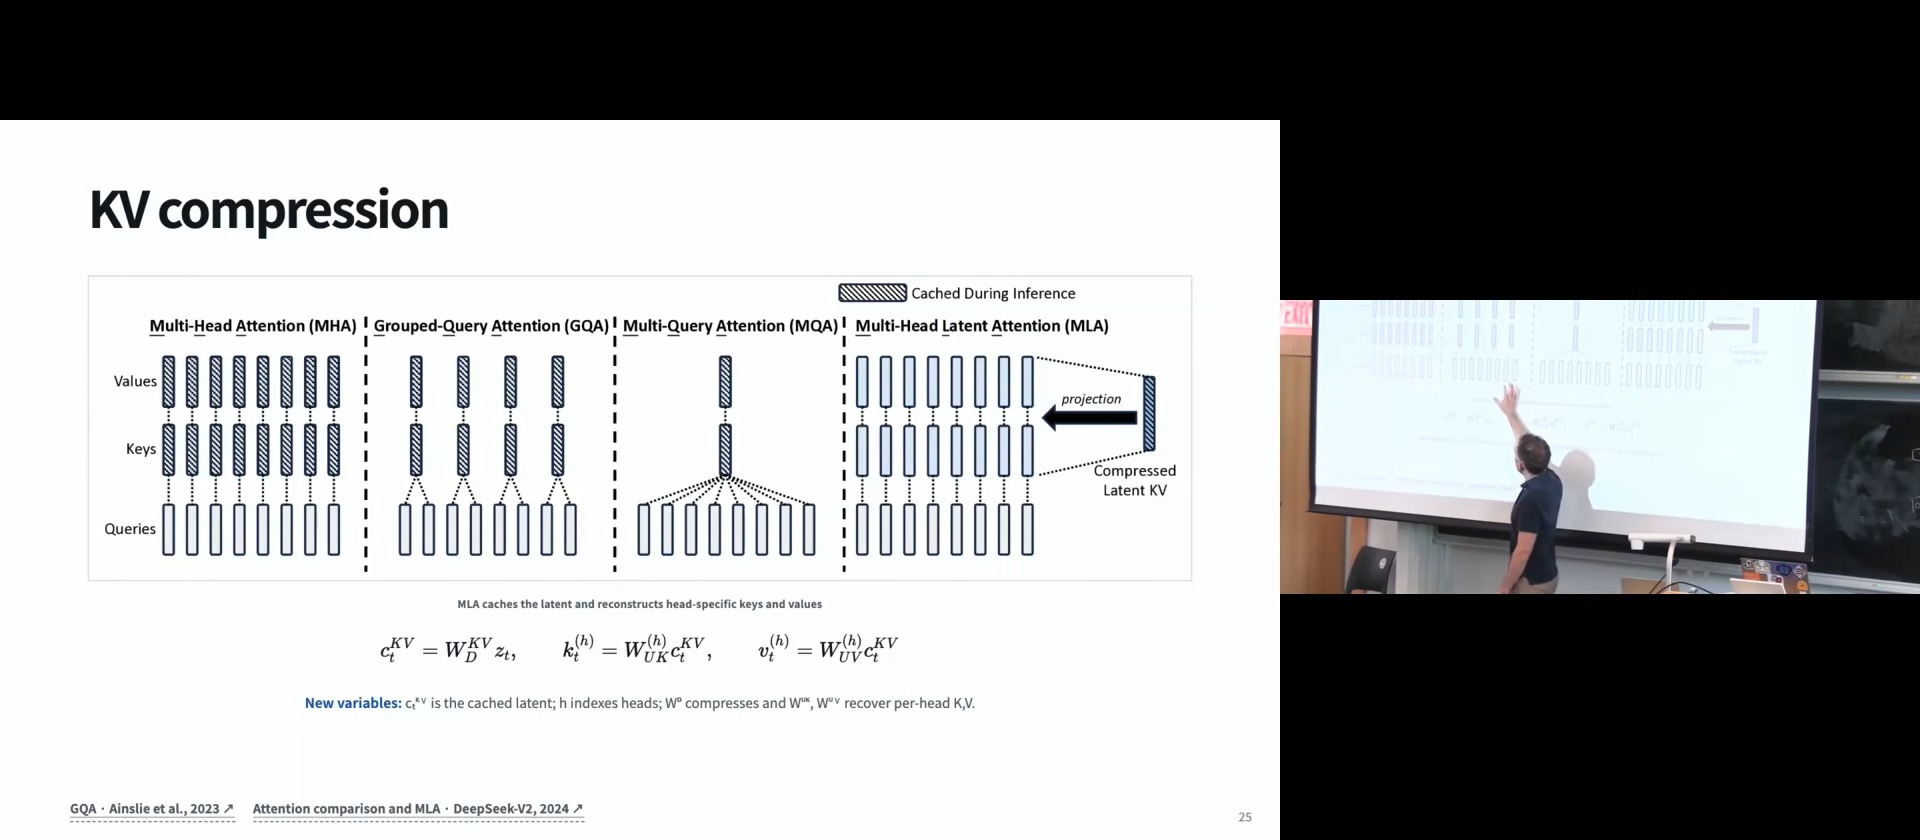
\includegraphics[width=\textwidth]{figures/fig_17_kv_compression.jpg}
\caption{KV 压缩：GQA/MQA 减少键值头数，MLA 缓存压缩 latent 再按头重建 K/V\vtag}
\end{figure}
\srcnote{00:34:15--00:34:29}

\subsection{本章小结}
稀疏注意力在“看多少”上做文章：固定模式便宜但可能错过，内容相关自适应但依赖选择器；KV 压缩在“存多少”上做文章：GQA/MQA 减少键值头数，MLA 缓存压缩 latent。架构层的三条路线（局部状态、稀疏全局、压缩缓存）到此齐了，它们共同把百万级上下文变成可服务的问题。下一节换一条战线：模型不是天生就能用长窗口，长上下文需要专门的训练过程。

\section{长上下文训练（一）：位置编码与长度扩展}

\subsection*{本节回答的问题}
为什么把窗口直接开大不能得到长上下文能力？训练分哪几个阶段，位置编码在长度外推中扮演什么角色？

\subsection{从短到长：三段式课程}

长上下文的第一个训练障碍是数据：长度达到 128K 的连贯文本在互联网上并不多，超过这个量级就接近“整本书”。因此训练通常分三步：先用大量廉价数据做\textbf{短预训练}（4K 到 8K），再用较长文档做\textbf{继续训练}（32K 到 128K），最后用长文档、任务轨迹与合成课程做\textbf{长适配}（128K 以上）。

\begin{figure}[H]
\centering
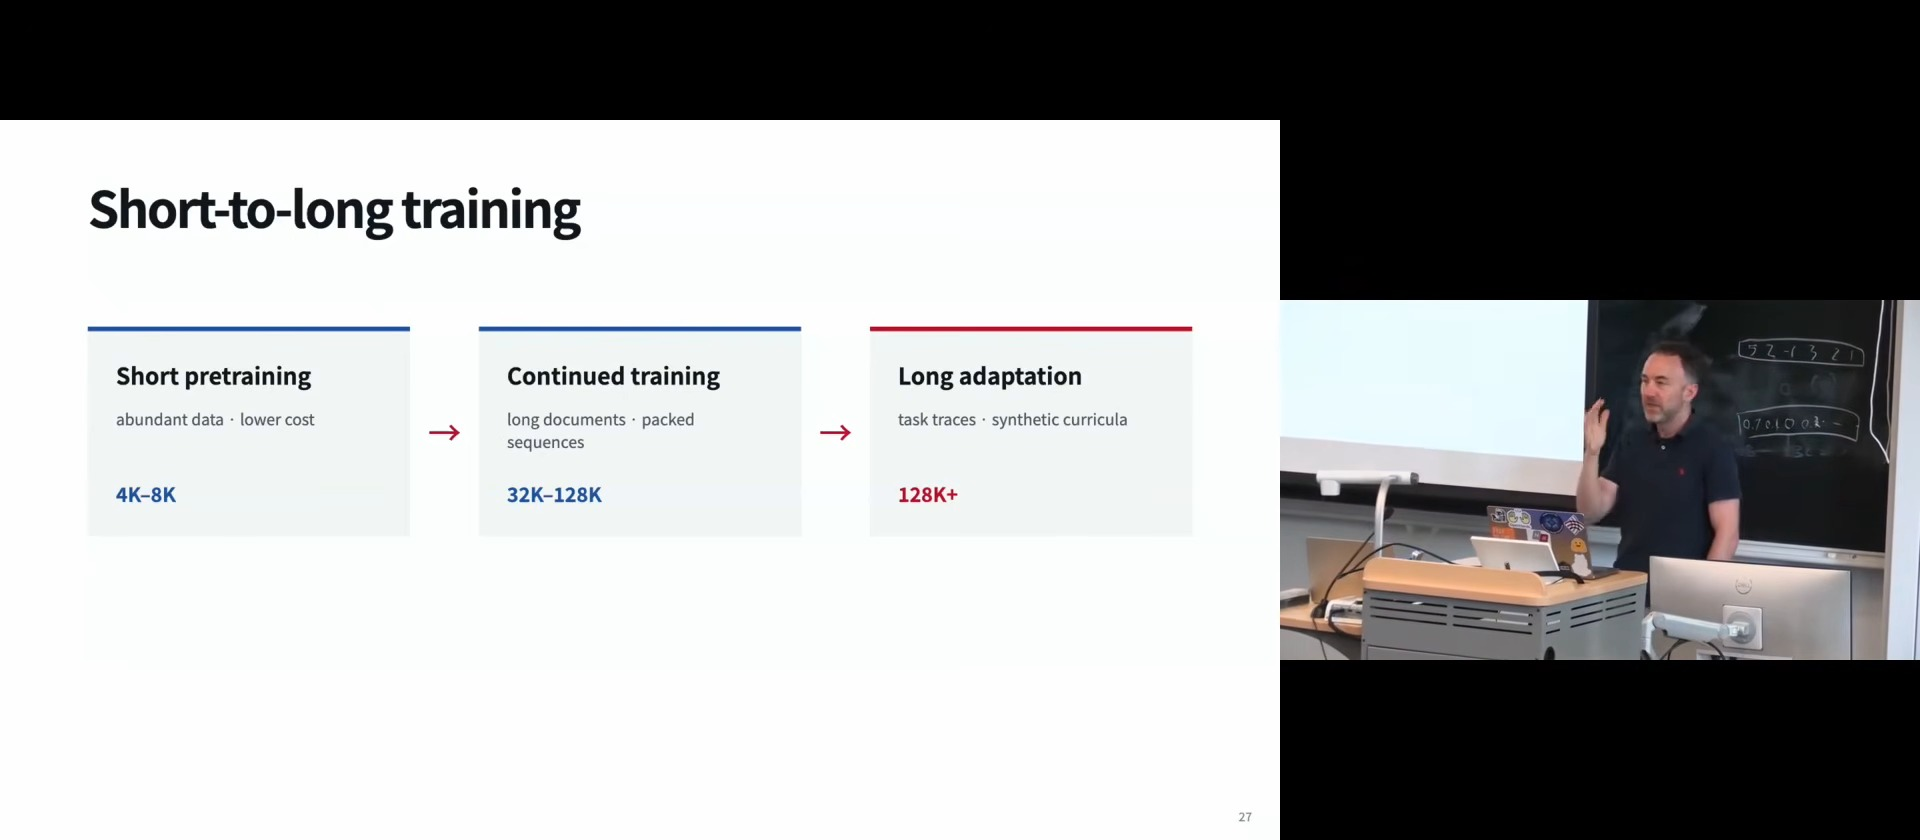
\includegraphics[width=\textwidth]{figures/fig_18_short_to_long.jpg}
\caption{短到长训练：short pretraining 4K--8K、continued training 32K--128K、long adaptation 128K+\vtag}
\end{figure}
\srcnote{00:37:15--00:37:29}

讲者提醒 packed sequences 只解决效率：把多篇短文档拼进一个序列能让模型学会处理靠近窗口末尾的位置，但拼进来的文档之间不应互相注意，因此它教不会“跨文档的全局连贯”。要教长上下文，还是需要真正连贯的长文档。

\subsection{位置编码：RoPE 与 NoPE}

绝对位置编码给每个位置加一个固定的位置向量：

\[
z_t=E[x_t]+p_t
\]

\begin{itemize}
\item $x_t$：第 $t$ 个位置的 token id；$E$：词嵌入表；
\item $p_t$：由 $\sin/\cos$ 生成的位置向量；$z_t$：送进第一层的状态。
\end{itemize}

旋转位置编码（RoPE）改成对查询与键做旋转，让注意力分数只依赖相对位移：

\[
q_i=R(i)\,q_i,\qquad k_j=R(j)\,k_j,\qquad
q_i^{\top}k_j=q_i^{\top}R(j-i)\,k_j
\]

\begin{itemize}
\item $R(t)$：按角度 $t\theta$ 构造的块对角旋转矩阵；
\item 旋转后两者的内积只通过 $j-i$ 依赖位置差，因此“相距多远”比“绝对在哪儿”更重要；
\item 值与注意力公式不变，只替换 $Q$、$K$。
\end{itemize}

\begin{figure}[H]
\centering
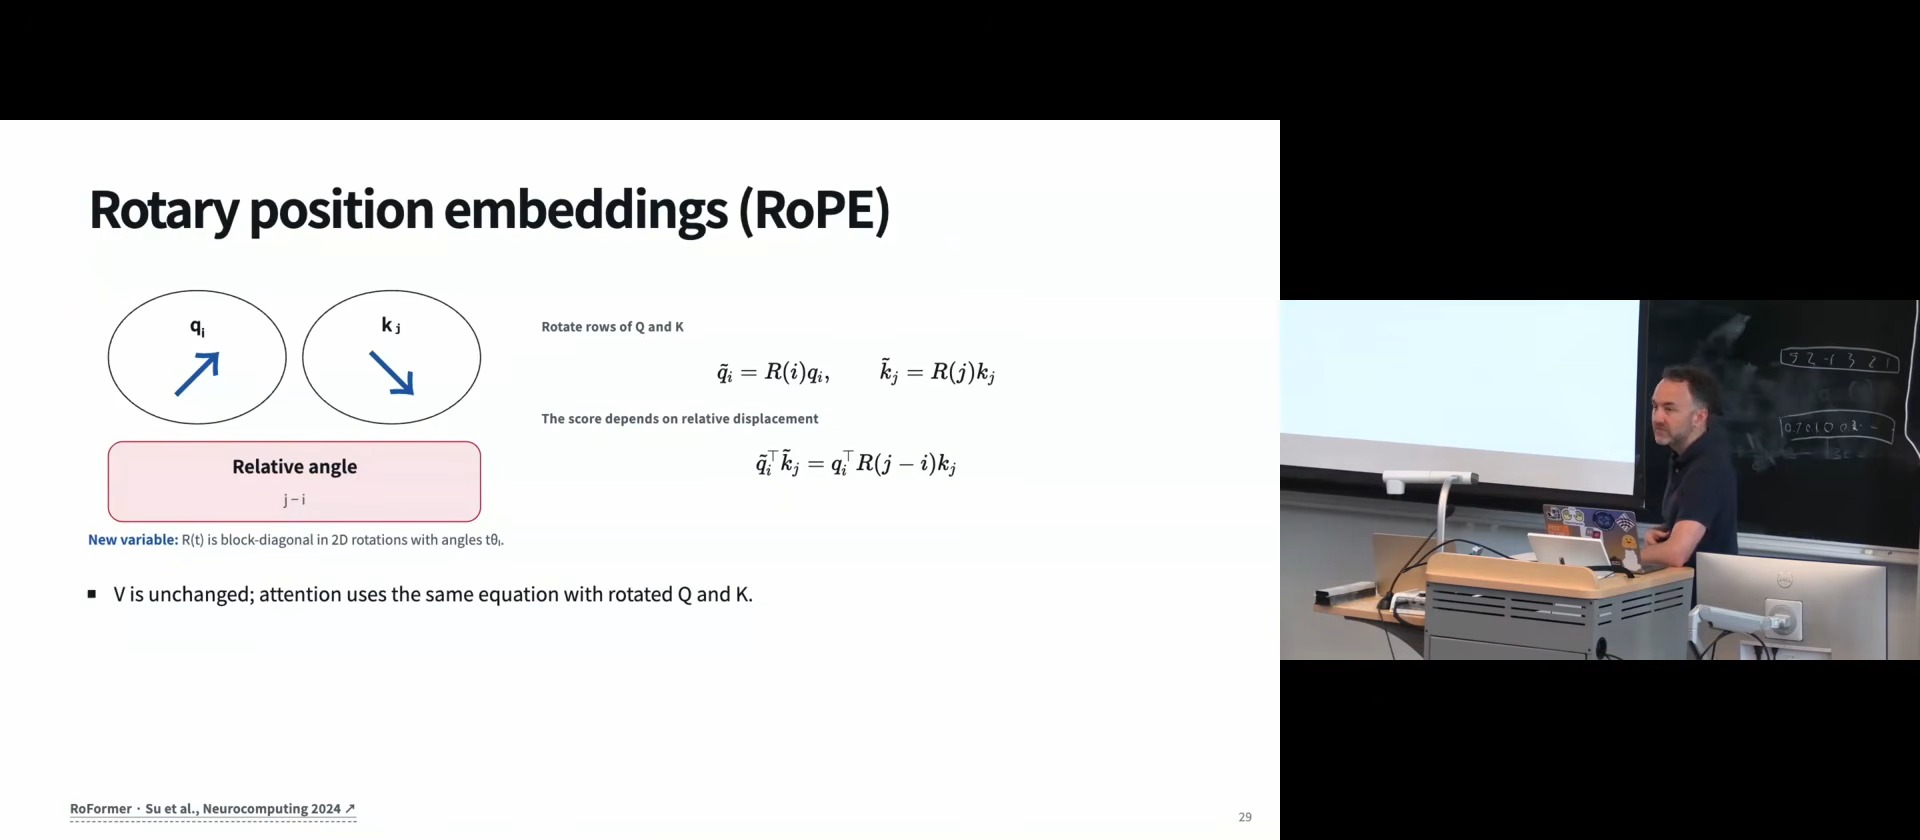
\includegraphics[width=\textwidth]{figures/fig_19_rope.jpg}
\caption{RoPE：对 Q、K 逐行旋转，分数只依赖相对位移 $q_i^{\top}R(j-i)k_j$\vtag}
\end{figure}
\srcnote{00:39:30--00:39:44}

讲者随后给了一个反直觉的结论：在自回归 Transformer 里，甚至可以完全不使用位置编码（NoPE），第一层只输入 $z_t=E[x_t]$。

\[
A=\operatorname{softmax}\!\left(\frac{QK^{\top}}{\sqrt{d_k}}+M\right),\qquad O=AV
\]

\begin{itemize}
\item 因果掩码 $M$ 让位置 $t$ 只能看到 $1\ldots t$，每个位置看到的“历史长度”本身就不一样；
\item 因此即使两个相同 token 的嵌入完全相同，它们在第一次注意力后就已经因为可见范围不同而区分开；
\item 在非自回归模型里所有位置互相可见，这个论证不成立，仍然需要位置编码。
\end{itemize}

\begin{figure}[H]
\centering
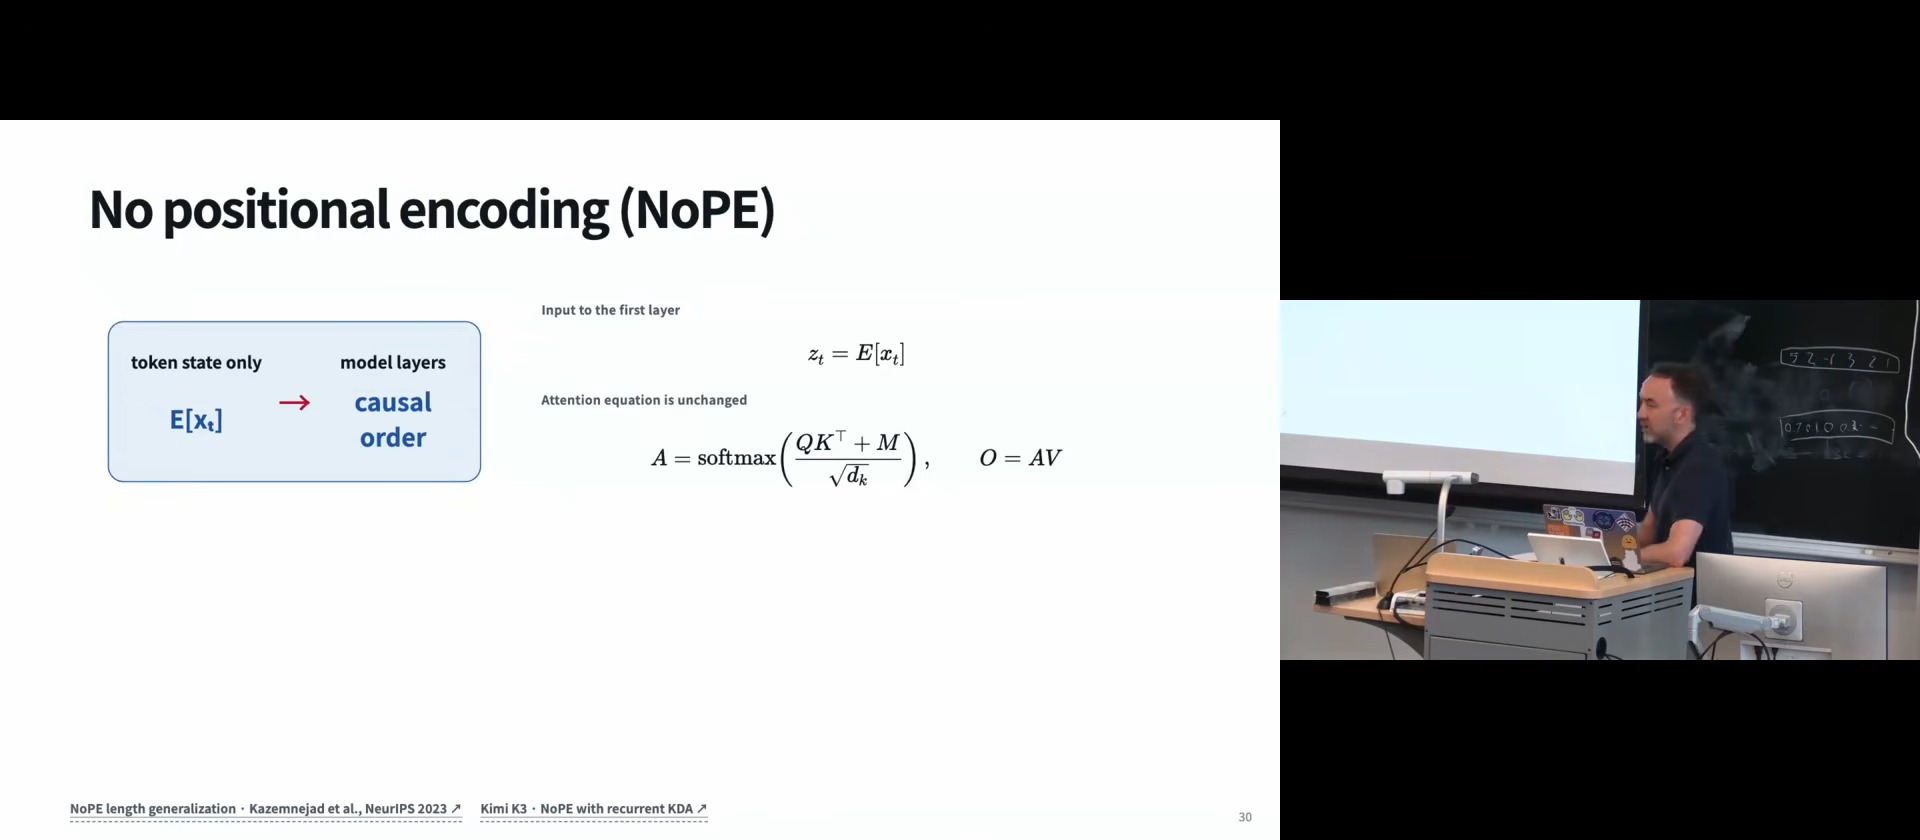
\includegraphics[width=\textwidth]{figures/fig_20_nope.jpg}
\caption{NoPE：第一层只输入 token 状态，顺序由因果计算（或循环动态）隐式给出\vtag}
\end{figure}
\srcnote{00:40:00--00:40:14}

\begin{importantbox}{“没有位置编码会分不清顺序”是过时的担忧}
这条结论依赖结构而不是玄学：因果掩码让每个位置的计算路径不同，带衰减的循环状态（如 Gated DeltaNet、Mamba）也让每个位置的表示随历史变化。讲者的幻灯片显示，今天主流模型的位置方案大约一半一半——部分 RoPE、完全 NoPE、或者依赖循环动态的隐式顺序。
\end{importantbox}

\subsection{长度扩展：位置插值与 YaRN}

位置编码解决了“相对距离”，但没有解决“训练时没见过那么远”。若训练只用长度 $L$，推理直接拉到 $sL$，模型从未见过距离超过 $L$ 的两个位置互相注意。位置插值的做法是把目标位置按比例压回熟悉的区间：

\[
L'=sL,\qquad R(t)\ \rightarrow\ R\!\left(t/s\right)
\]

\begin{itemize}
\item $L$、$L'$：原始与目标上下文上限；$s=L'/L$：扩展倍数；
\item 用 $t/s$ 计算旋转角，使目标位置 $t$ 落回预训练见过的相位范围；
\item 等价地在 RoPE 的温度参数上除以 $s$，即“拉伸”整条位置轴。
\end{itemize}

\begin{figure}[H]
\centering
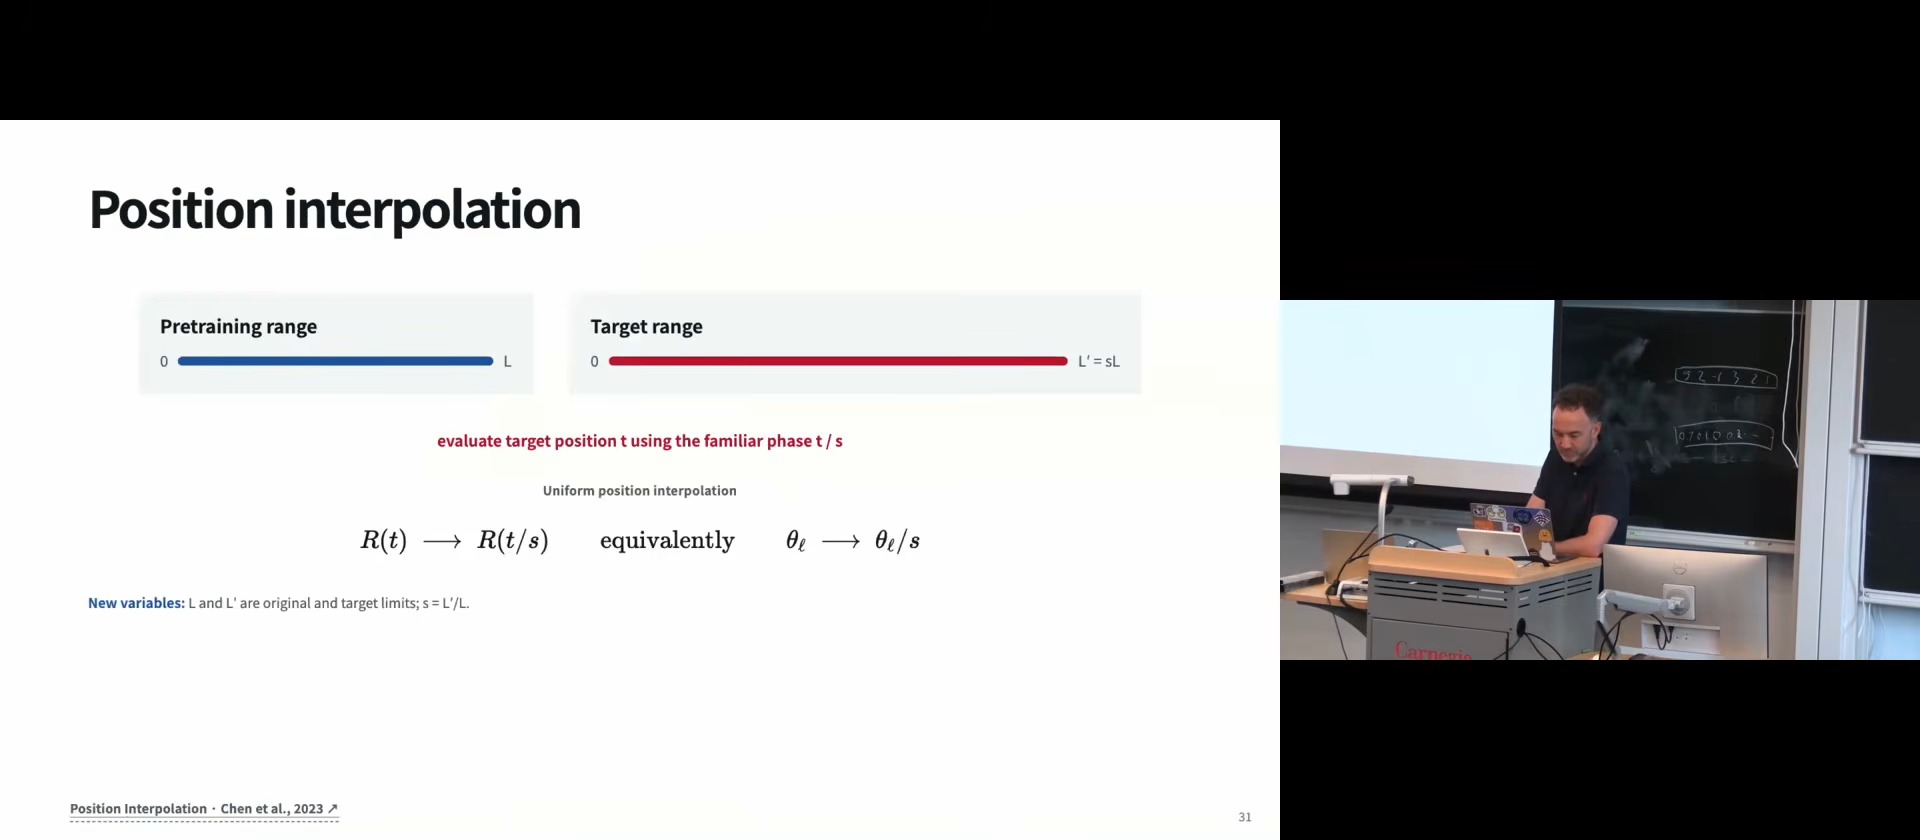
\includegraphics[width=\textwidth]{figures/fig_21_position_interp.jpg}
\caption{位置插值：把训练范围 $L$ 拉伸到 $L'=sL$，用 $R(t)\to R(t/s)$ 复用熟悉的相位\vtag}
\end{figure}
\srcnote{00:42:30--00:42:44}

均匀插值会同时改变所有频率，YaRN 改成按频率分段：长波长（决定全局位置）完全插值，中段线性混合，短波长（决定局部相位）尽量保留；同时给注意力温度一个随 $s$ 变化的修正。

\[
A=\operatorname{softmax}\!\left(\frac{QK^{\top}}{T\sqrt{d_k}}+M\right),\qquad
T=\frac{1}{0.1\ln s+1}
\]

\begin{itemize}
\item 分段系数 $\gamma$ 从长波长的 0 渐变到短波长的 1，决定该频率插值多少；
\item $T$：注意力温度，扩展倍数越大，$T$ 越小，用来抵消注意力分布随距离变平的趋势；
\item 这样既保留局部相位的分辨率，又让远处位置落在已学过的范围里。
\end{itemize}

\begin{figure}[H]
\centering
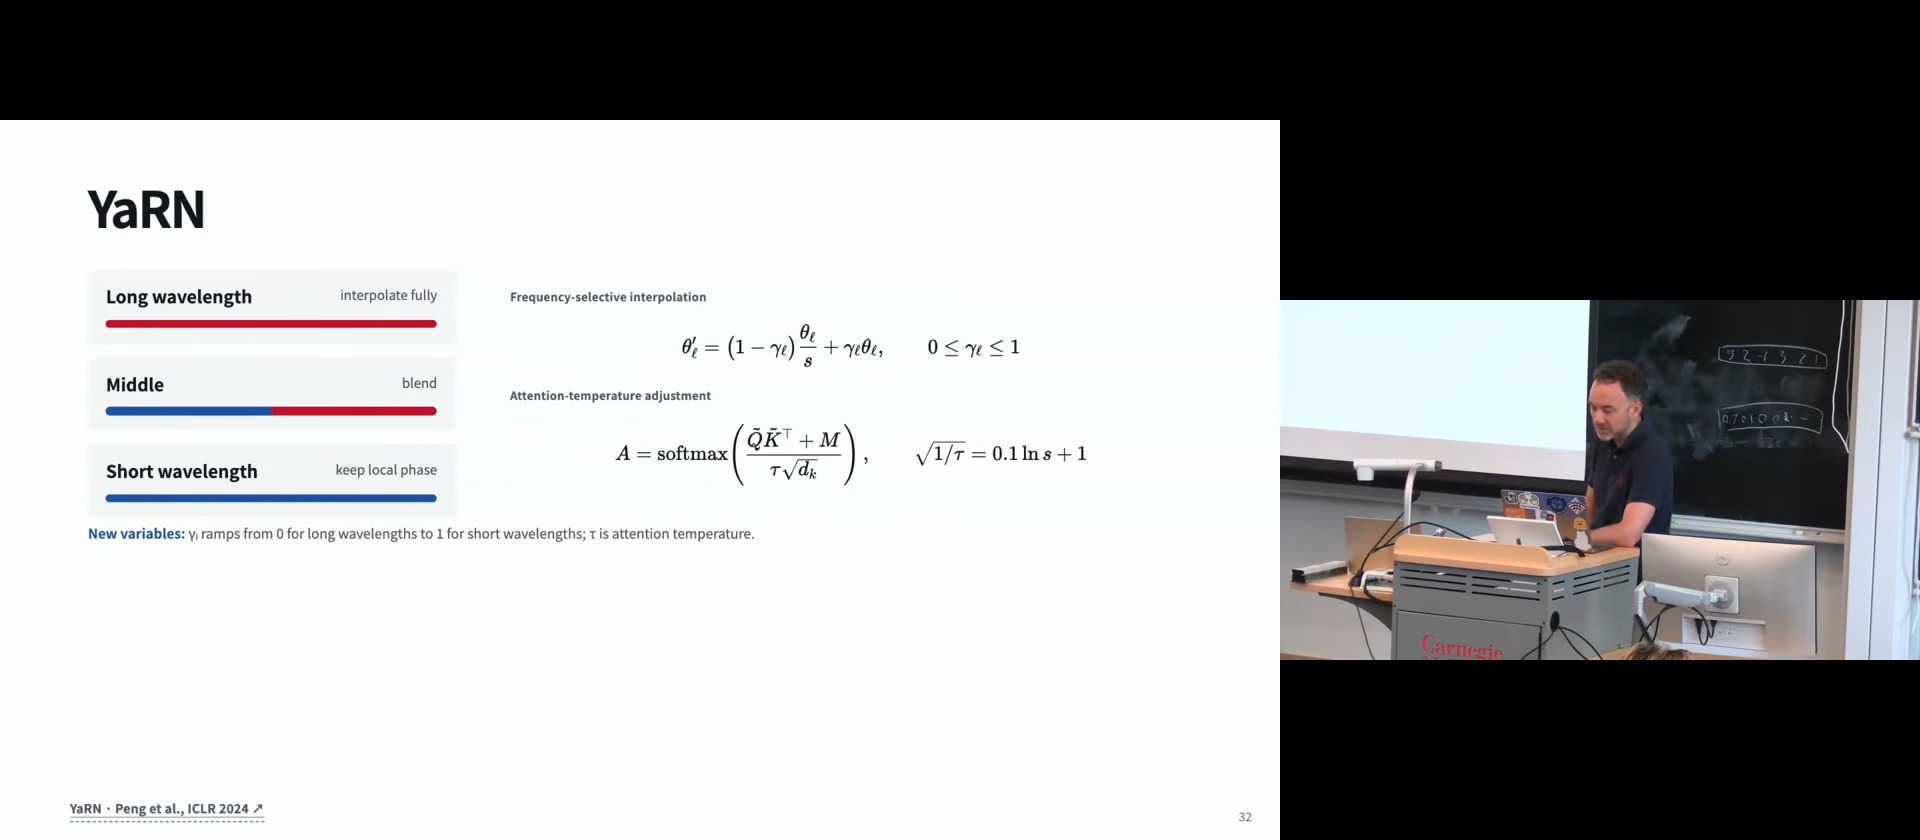
\includegraphics[width=\textwidth]{figures/fig_23_yarn.jpg}
\caption{YaRN：按频率分段插值（长波长全插值、中段混合、短波长保留）并调整注意力温度\vtag}
\end{figure}
\srcnote{00:45:30--00:45:44}

各家的具体路径并不相同。幻灯片列出的一组做法是：Qwen3.8-Flash-Next 用部分 RoPE 加 YaRN 扩到 1M；DeepSeek V4 采用 4K 到 16K、64K、1M 的渐进课程加 YaRN，不做 RoPE 重标定；GLM-5.3-Flash 在主注意力里用 NoPE；Kimi K3 用 NoPE 配合循环 KDA，课程是 8K 到 64K、256K、1M；Nemotron3Ultra 训练与评测都在长长度上，依赖 Mamba 的隐式顺序；Inkling 使用相对位置编码。

\begin{figure}[H]
\centering
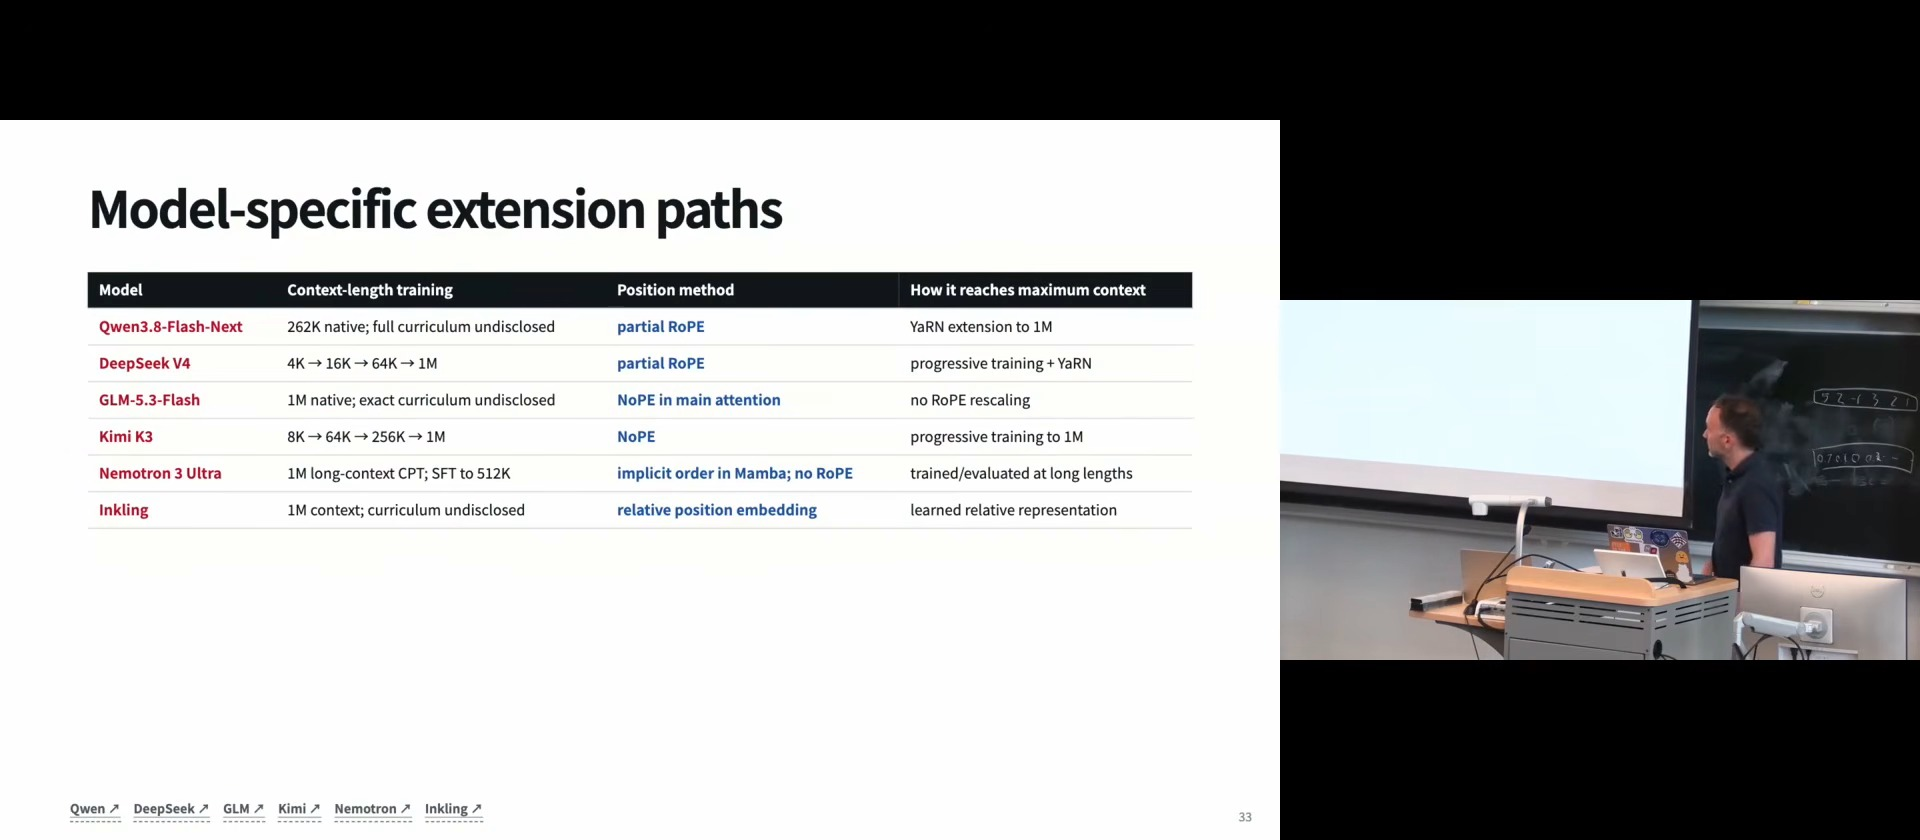
\includegraphics[width=\textwidth]{figures/fig_22_model_extension_table.jpg}
\caption{各模型扩展路径：部分 RoPE+YaRN、NoPE、显式长长度训练与相对位置编码并存\vtag}
\end{figure}
\srcnote{00:43:00--00:43:14}

\begin{knowledgebox}{为什么同一个问题会有这么多答案}
位置编码的选择与局部状态机制耦合：一旦模型大量使用带衰减的循环层，顺序信息已经由状态更新携带，位置编码的必要性就下降；反过来，纯注意力模型更依赖显式的相对位置。因此“该不该用 RoPE”要在整套架构里回答。
\end{knowledgebox}

\subsection{本章小结}
长上下文训练走“短预训练、继续训练、长适配”三段课程，因为超长连贯文本稀缺；位置编码从绝对位置走到 RoPE 的相对位移，再到自回归模型里可用的 NoPE；长度扩展则用位置插值把新位置压回熟悉区间，YaRN 进一步按频率分段并调整注意力温度。位置问题解决后，下一个现实问题是：训练数据从哪里来，以及几百万 token 的序列怎么放进多卡。

\section{长上下文训练（二）：数据与上下文并行}

\subsection*{本节回答的问题}
真正的长上下文训练数据有哪几类，各教什么能力？把一条超长序列拆到多张卡上，代价和难点分别在哪里？

\subsection{四类训练数据}

讲者把长上下文数据分成四类。\textbf{打包示例}把多篇文档拼进一个窗口，token 利用率高，但要注意文档边界与跨样本泄漏；\textbf{长文档}（书籍、代码库、多文档语料）具有天然的连贯结构；\textbf{agent 轨迹}由动作与观察组成，教的是长程恢复、状态跟踪与工具使用；\textbf{合成任务}把证据与干扰项放在设计好的位置上，用来测受控的依赖关系。

\begin{figure}[H]
\centering
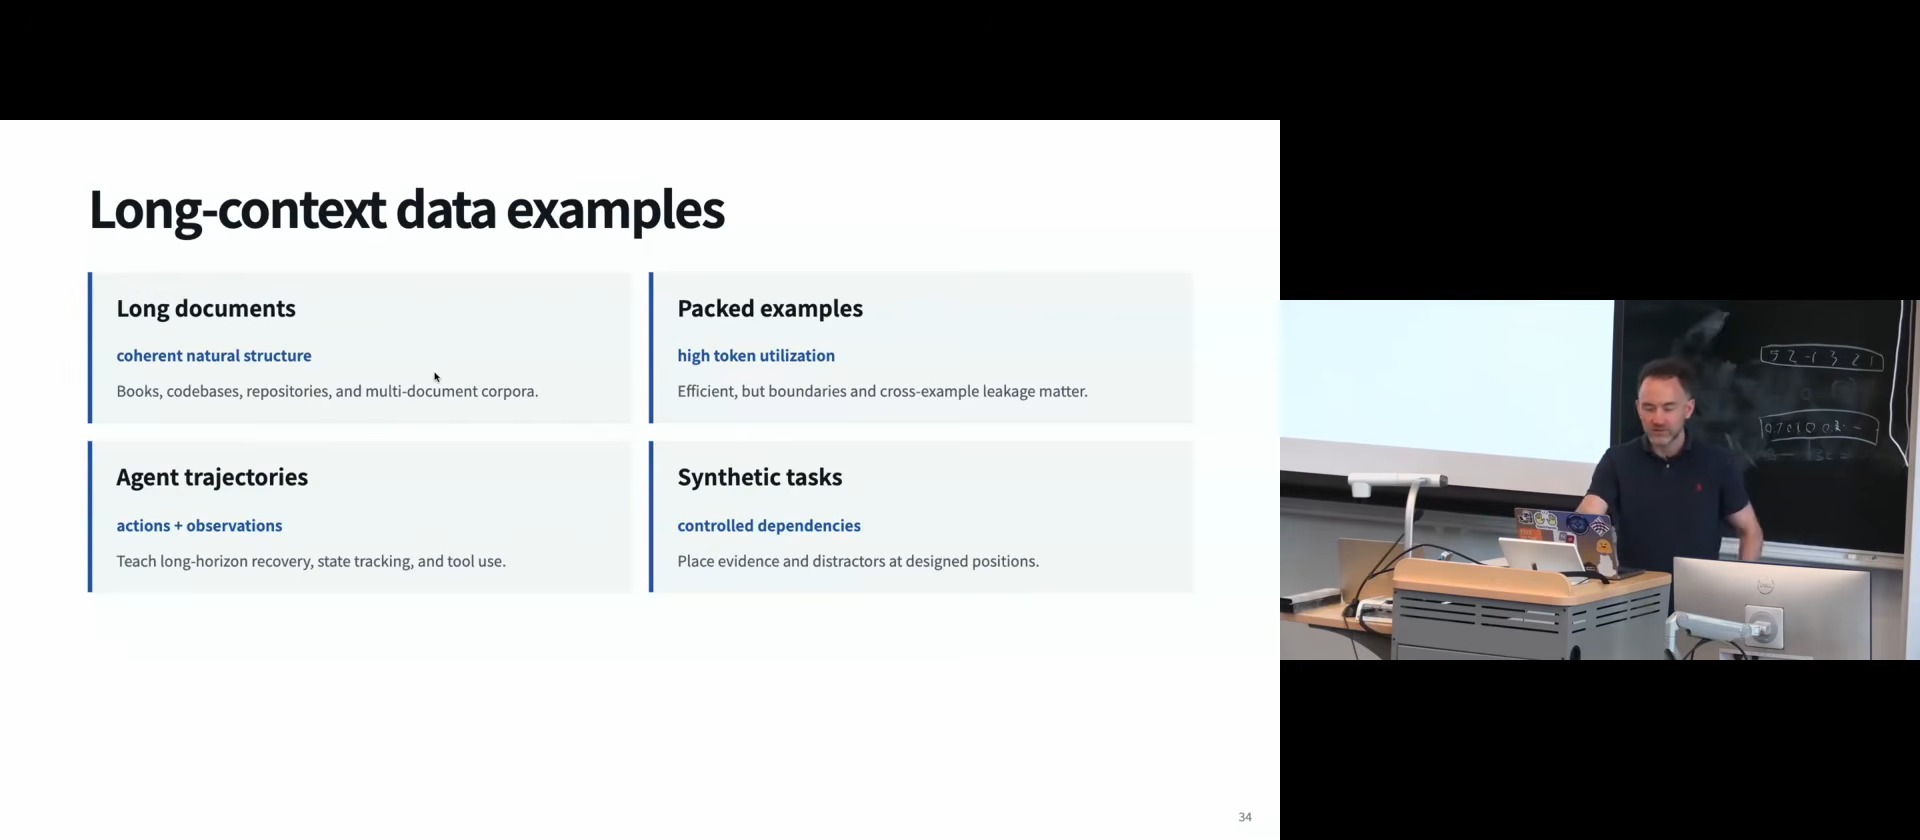
\includegraphics[width=\textwidth]{figures/fig_24_data_examples.jpg}
\caption{四类长上下文数据：packed examples、long documents、agent trajectories、synthetic tasks\vtag}
\end{figure}
\srcnote{00:47:30--00:47:44}

公开模型会披露数据来源，但通常不披露配比与训练策略。幻灯片给出的几个例子说明课程长度和数据来源是配套的：

\begin{table}[H]
\centering
\small
\begin{tabular}{@{}p{3.2cm}p{3.6cm}p{7.4cm}@{}}
\toprule
模型 & 长度课程 & 数据来源与构造监督 \\
\midrule
Kimi K3 & 8K 到 64K、256K、1M & 清洗并上采样的文档与视频，全上下文排列的多模态子任务 \\
GLM-5 & 32K 到 128K、200K & 仓库文件、issue 与 PR，合成依赖和 agent 轨迹 \\
Nemotron3Ultra & 1M 长度的继续预训练 & 长文档问答，之后做 agentic 后训练 \\
DeepSeek V4 & 4K 到 16K、64K、1M & 科学论文与技术报告等长文档 \\
\bottomrule
\end{tabular}
\caption{各模型的长上下文数据配方（据幻灯片整理）}
\end{table}

\begin{figure}[H]
\centering
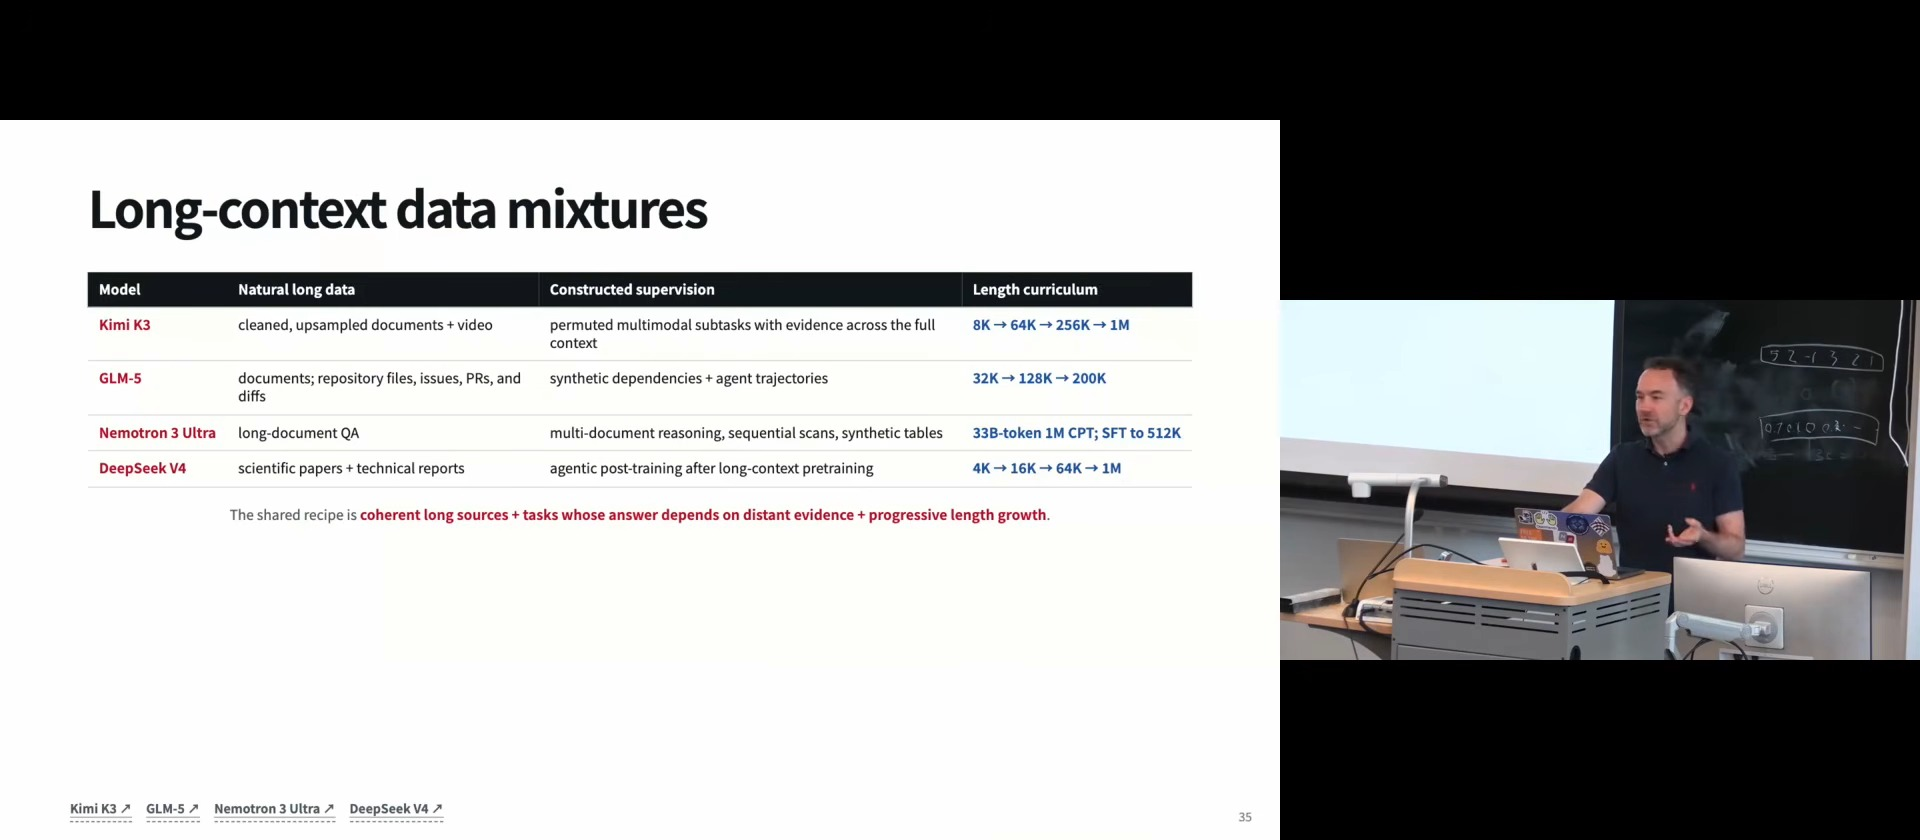
\includegraphics[width=\textwidth]{figures/fig_25_data_mixtures.jpg}
\caption{数据配方表：Kimi K3 走 8K 到 1M 的课程，GLM-5 到 200K，Nemotron 做 1M 继续预训练\vtag}
\end{figure}
\srcnote{00:48:15--00:48:29}

\subsection{上下文并行：把序列切开放在多张卡上}

一条百万 token 的序列，单卡显存放不下激活与 KV。上下文并行把序列按块切到 $P$ 张设备上：每张设备负责一部分键值，然后沿环把键值块依次传给下一张设备，每个查询在自己的块与轮转到的所有键值块上做注意力，最后回到起始设备。这就是 Ring Attention 的基本形态。

\[
\text{设备内存}=O\!\left(\frac{n\,d_k}{P}\right),\qquad
\text{总工作量}=O\!\left(n^2 d_k\right)\ \text{（精确而非近似）}
\]

\begin{itemize}
\item $n$：序列长度；$d_k$：键宽；$P$：设备数；
\item 注意力本身仍然是精确的，切分只是把内存分布到多张卡上，不改变计算结果；
\item 通信与分块注意力重叠进行，因此额外开销主要取决于互连带宽。
\end{itemize}

\begin{figure}[H]
\centering
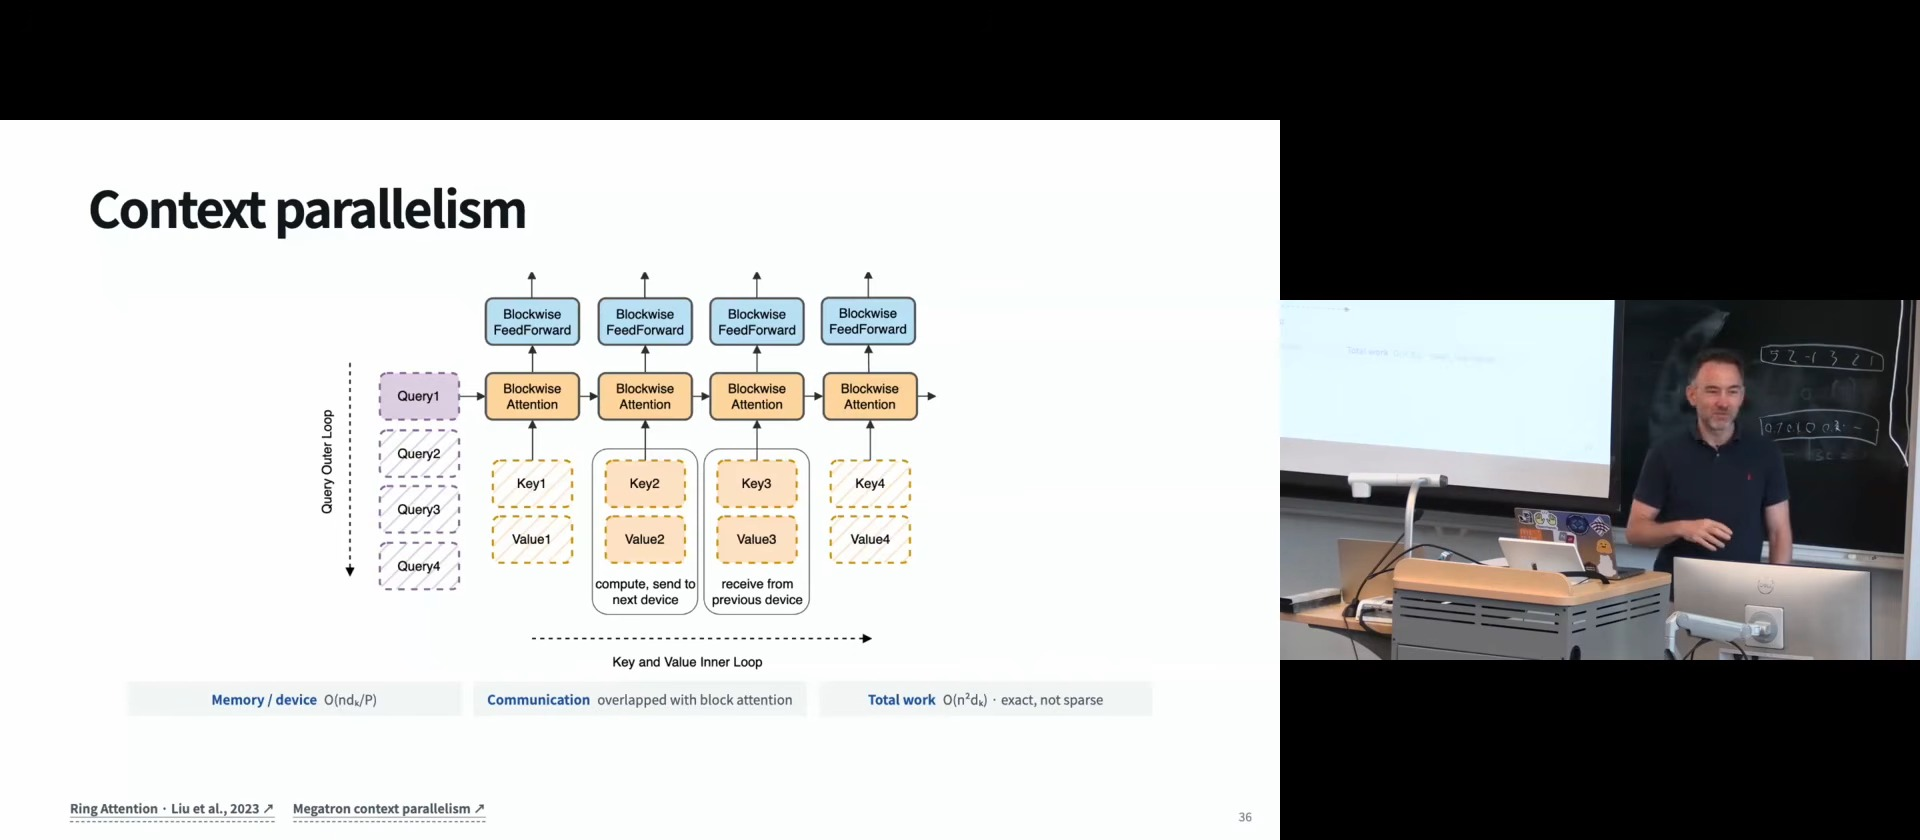
\includegraphics[width=\textwidth]{figures/fig_26_context_parallel.jpg}
\caption{上下文并行：键值块在设备间轮转，每设备内存约 $O(n d_k/P)$，计算仍是精确的\vtag}
\end{figure}
\srcnote{00:49:45--00:49:59}

讲者说上下文并行在 32K 以上就变得重要，但它同时也是长上下文工程里最容易“卡住”的地方：模型研究想要新的状态更新（例如 Gated DeltaNet），系统团队则需要为它写出支持反向传播、支持上下文并行的 kernel。讲者分享了自己的经历——曾想把一个较小的 Qwen 模型用上下文并行训练，却发现社区里根本没有 Gated Delta Net 的现成 kernel，只能自己实现或换方案；而标准注意力与滑动窗口这类规则结构，kernel 要容易得多。

\begin{warningbox}{新机制的表达力是模型侧的收益，也是系统侧的负债}
注意力机制越“非标准”（逐通道衰减、稀疏选择、交错分支），越难获得高效的序列并行实现。选型时要把“论文里的效果”和“我能不能在多卡上练起来、服务起来”放在同一张表里比较。
\end{warningbox}

\subsection{本章小结}
长上下文数据分四类，打包示例省算力但教不会跨文档连贯，长文档与代码库提供自然连贯结构，agent 轨迹与合成任务负责长程能力；各家模型把长度课程与数据来源配套设计。把超长序列放进多卡依靠上下文并行，它保持精确计算、把内存摊到 $P$ 张卡，但代价是通信与“新机制缺少 kernel”的工程摩擦。至此训练侧的三个问题——位置、数据、并行——讲完，下一节回到服务侧最直接的省钱手段：KV cache 复用。
\section{KV cache：复用、成本与命中率}

\subsection*{本节回答的问题}
为什么第 $t$ 轮的输入里绝大部分是可以不重算的？缓存的收益有多大，账单上的“缓存输入”为什么能便宜一个数量级？

\subsection{缓存是怎么省下 prefill 的}

在第 2 节的服务栈里，prefill 会把 prompt 的每个位置算出键值。到了下一轮，prompt 只是“上一轮的 prompt + 上一轮的输出 + 新的工具结果”。其中前面那一大段前缀与上一轮逐字节相同，它们的键值完全可以原样复用，只有新追加的部分需要重新算。

\[
N_{\text{new}}(t)=s,\qquad
N_{\text{prefix}}(t)=\sum_{i<t}s=s\,(t-1)
\]

\begin{itemize}
\item $N_{\text{new}}(t)$：第 $t$ 轮真正需要新算的 token 数，等于这一轮新增的历史；
\item $N_{\text{prefix}}(t)$：可以命中的历史前缀；到第 50 轮，前缀大约是新增输入的 50 倍；
\item 无缓存时每轮都要重算前缀，缓存后每轮只算新增部分。
\end{itemize}

\begin{figure}[H]
\centering
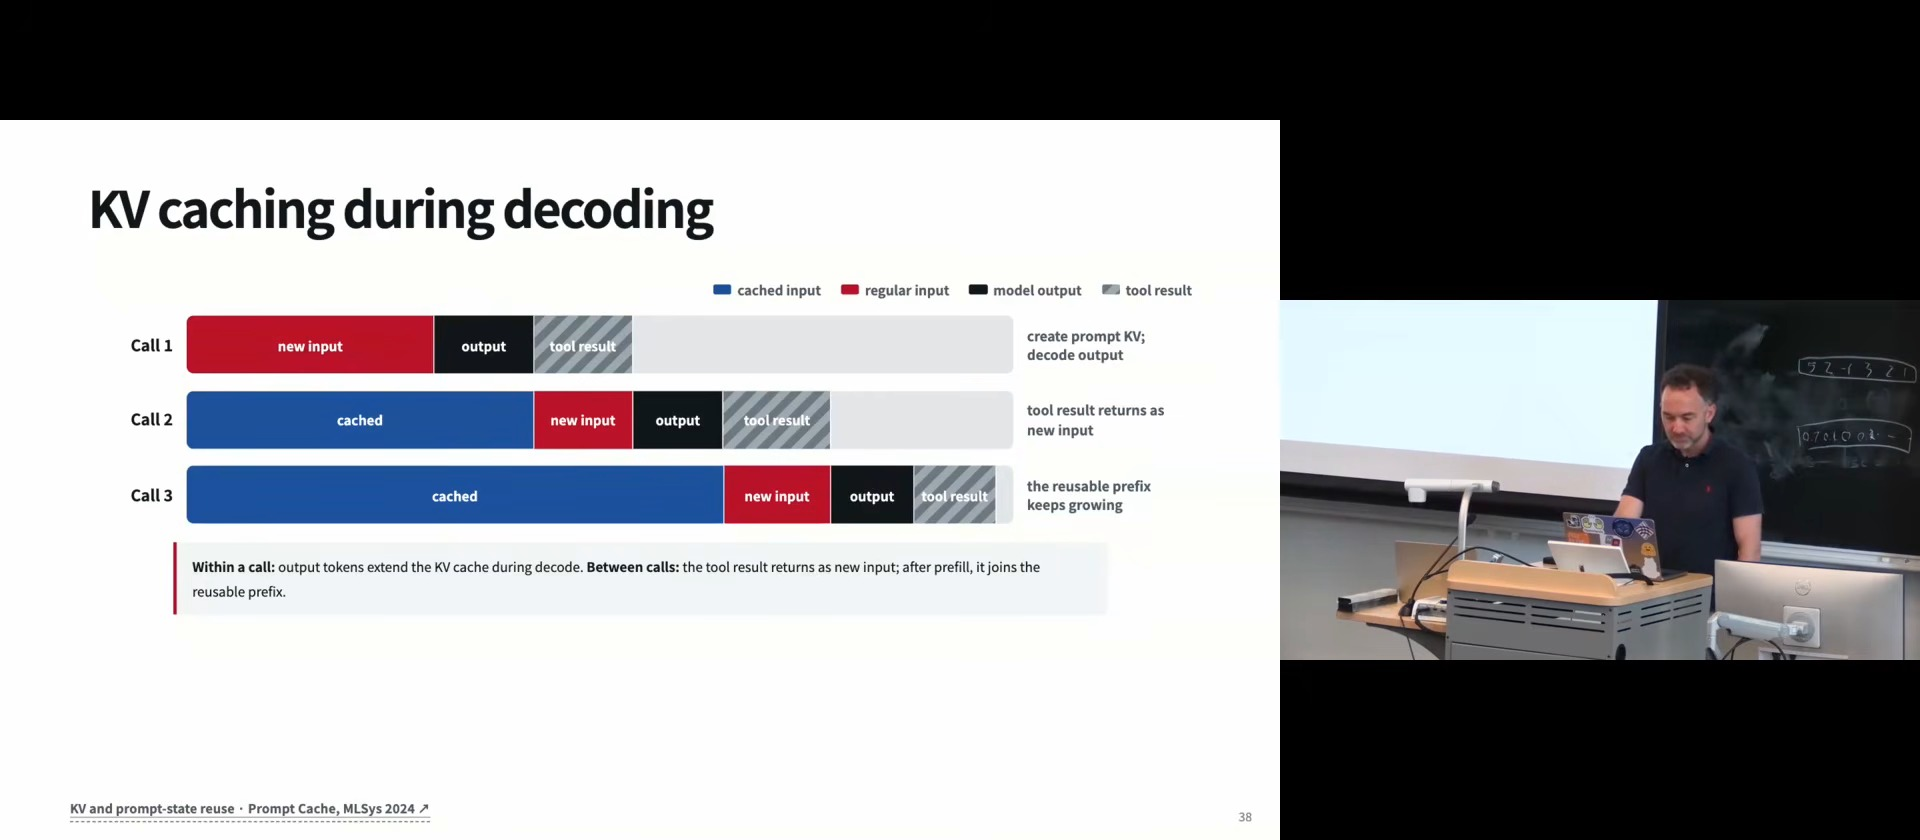
\includegraphics[width=\textwidth]{figures/fig_27_kv_caching.jpg}
\caption{KV 缓存：调用内输出扩展缓存，调用间 tool result 作为新输入、prefill 后并入可复用前缀\vtag}
\end{figure}
\srcnote{00:54:00--00:54:14}

\subsection{经验收益：从二次回到线性}

幻灯片引用的实测把“每轮从头 prefill”与“复用 KV”画在同一张图上：不缓存的每调用成本随序列长度呈二次增长，缓存之后近似线性；缓存带来的优势在 CPU、A40 与 RTX 4090 上都存在，且序列越长越明显。

\[
\text{无缓存成本}\ \propto\ \sum_{t=1}^{N}\left(P+s t\right),
\qquad
\text{缓存成本}\ \propto\ P+sN
\]

\begin{itemize}
\item 左侧是每轮重算全部前缀的累计成本，按 $N^2$ 增长；
\item 右侧只在第一轮算完整前缀，之后每轮只算新增的 $s$；
\item 差异不来自“某个算子变快”，而来自“同一段前缀只算一次”。
\end{itemize}

\begin{figure}[H]
\centering
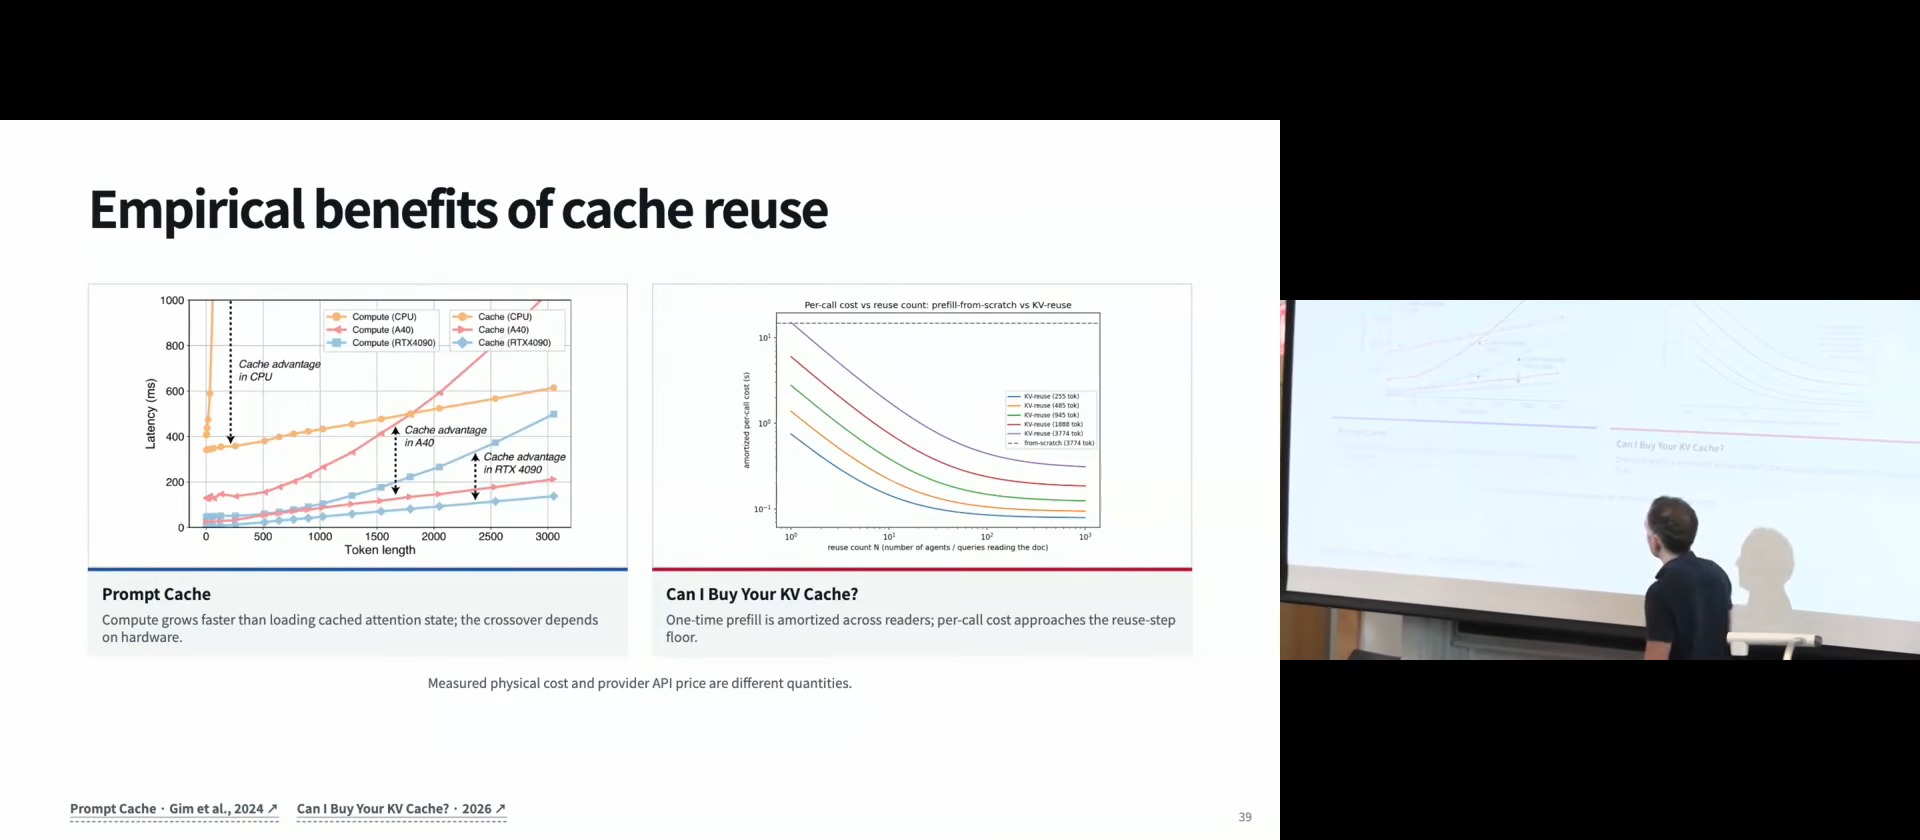
\includegraphics[width=\textwidth]{figures/fig_28_cache_benefit.jpg}
\caption{缓存复用的经验收益：每调用成本与延迟在 CPU、A40、RTX4090 上均随复用次数下降\vtag}
\end{figure}
\srcnote{00:54:30--00:54:44}

\subsection{价格：缓存输入约为常规输入的十分之一}

讲者从各家的公开定价里得出一个稳定规律：缓存命中（cache read）的单价约为常规输入的十分之一。幻灯片把若干模型的常规输入、缓存输入与输出单价并排列出；讲者同时提醒，”cached”只指缓存读取，写入缓存（cache creation）可能单独计费，而且同一家的价格还可能分平峰与高峰。

\[
\text{cost}=c_{\text{in}}N_{\text{in}}^{\text{new}}+c_{\text{cached}}N_{\text{cached}}+c_{\text{out}}N_{\text{out}}
\]

\begin{itemize}
\item $c_{\text{in}},c_{\text{cached}},c_{\text{out}}$：常规输入、缓存输入、输出的单价；
\item $N_{\text{cached}}$：命中的前缀 token 数，通常远大于 $N_{\text{in}}^{\text{new}}$；
\item 由于 $c_{\text{cached}}\approx 0.1\,c_{\text{in}}$、而 $c_{\text{out}}\approx 5\,c_{\text{in}}$，输出与缓存输入之间可以差到约 50 倍。
\end{itemize}

\begin{figure}[H]
\centering
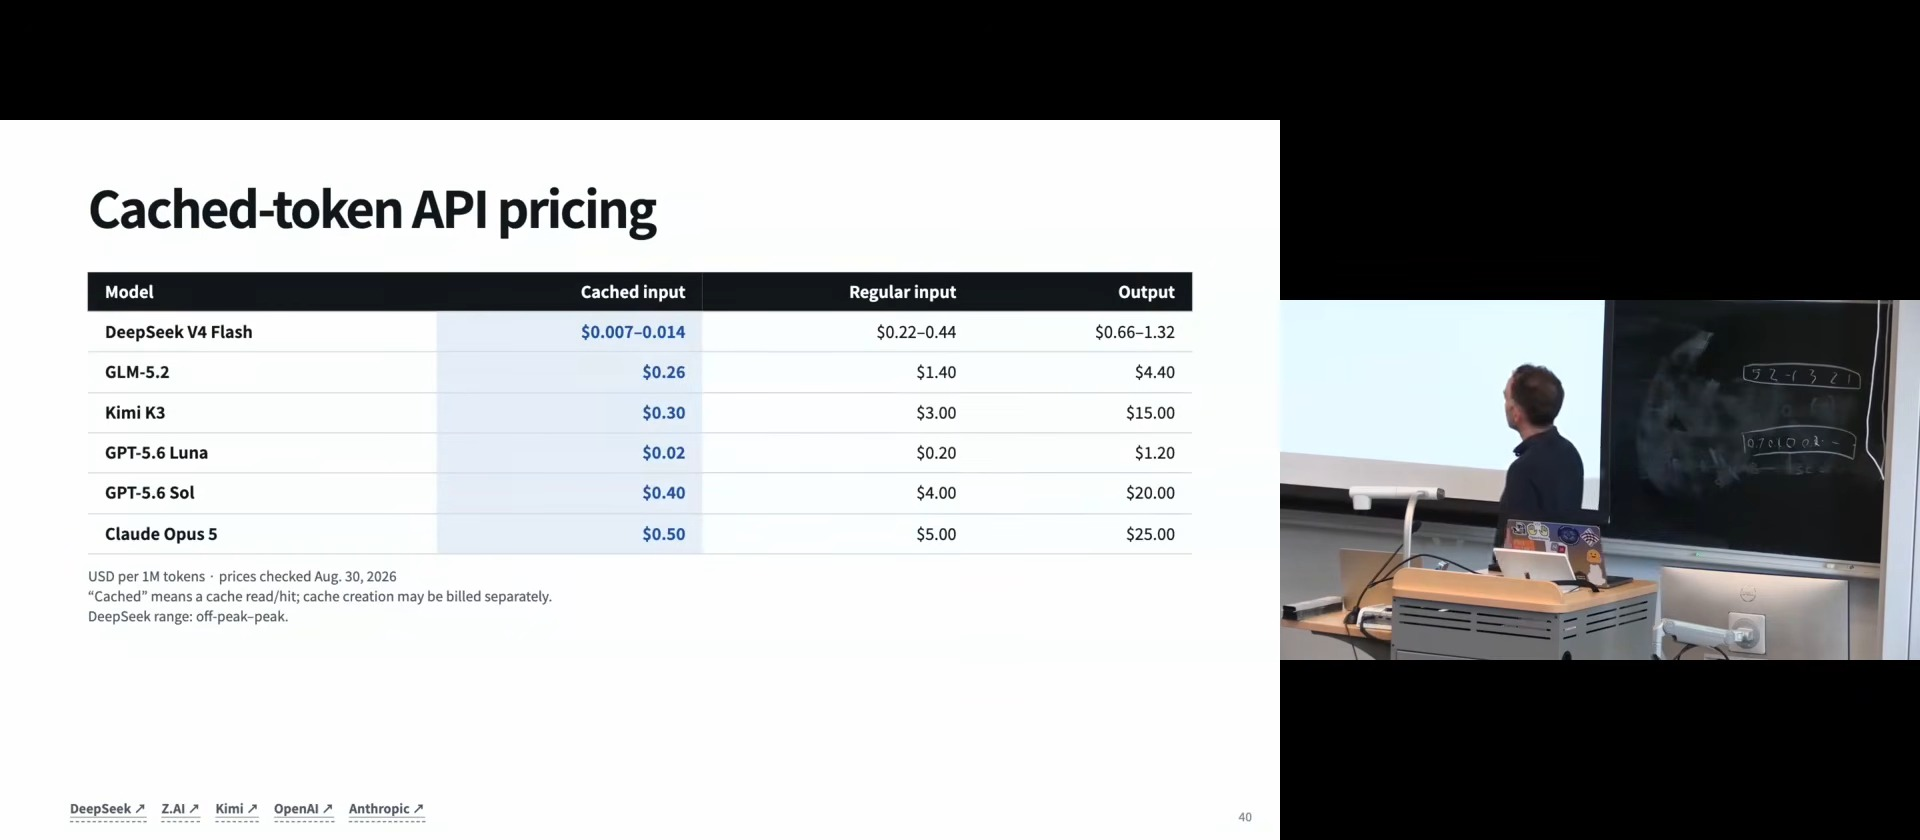
\includegraphics[width=\textwidth]{figures/fig_29_cached_pricing.jpg}
\caption{缓存输入定价：若干模型按常规输入、缓存输入与输出三列排出的单价（USD/百万 token）\vtag}
\end{figure}
\srcnote{00:55:00--00:55:14}

讲者现场问了“多高的缓存命中率算好”：课堂回答是 80\% 到 90\% 这一档，也有人提到 95\% 以上。
讲者自己的判断是命中率要到 90 到 95 这个区间才算健康，低于它就要检查是不是哪里打破了前缀。

\begin{importantbox}{把缓存命中率当成一等指标}
命中率不是服务商的内部指标，而是 agent 设计质量的直接体现：它决定了账单、TTFT 与可支持的会话长度。讲者的建议是把“缓存命中的 token 数、TTFT、驱逐情况”当成和成功率一样的常规监控项。
\end{importantbox}

\subsection{本章小结}
KV cache 让上一轮已经算过的前缀不必重算，把每轮成本从“前缀加新增”降到“只算新增”；经验上它把二次成本拉回线性，定价上缓存输入约为常规输入的十分之一，使得命中率成为 agent 的核心指标。下一节看支撑这套机制的基础设施，以及 harness 侧为了不破坏缓存必须遵守的纪律。

\section{缓存基础设施与 harness 纪律}

\subsection*{本节回答的问题}
服务端用什么结构管理成千上万条 KV 前缀？如果自己写 harness，哪些看似合理的做法会悄悄让缓存失效？

\subsection{PagedAttention：像管理内存页一样管理 KV}

vLLM 的主要技术贡献是把 KV cache 按物理块管理。每块保存固定数量的 token 的键值，逻辑上连续的序列通过一张 block table 映射到不连续的物理块，于是不同序列可以共享块、序列结束时可以整块回收。

\begin{figure}[H]
\centering
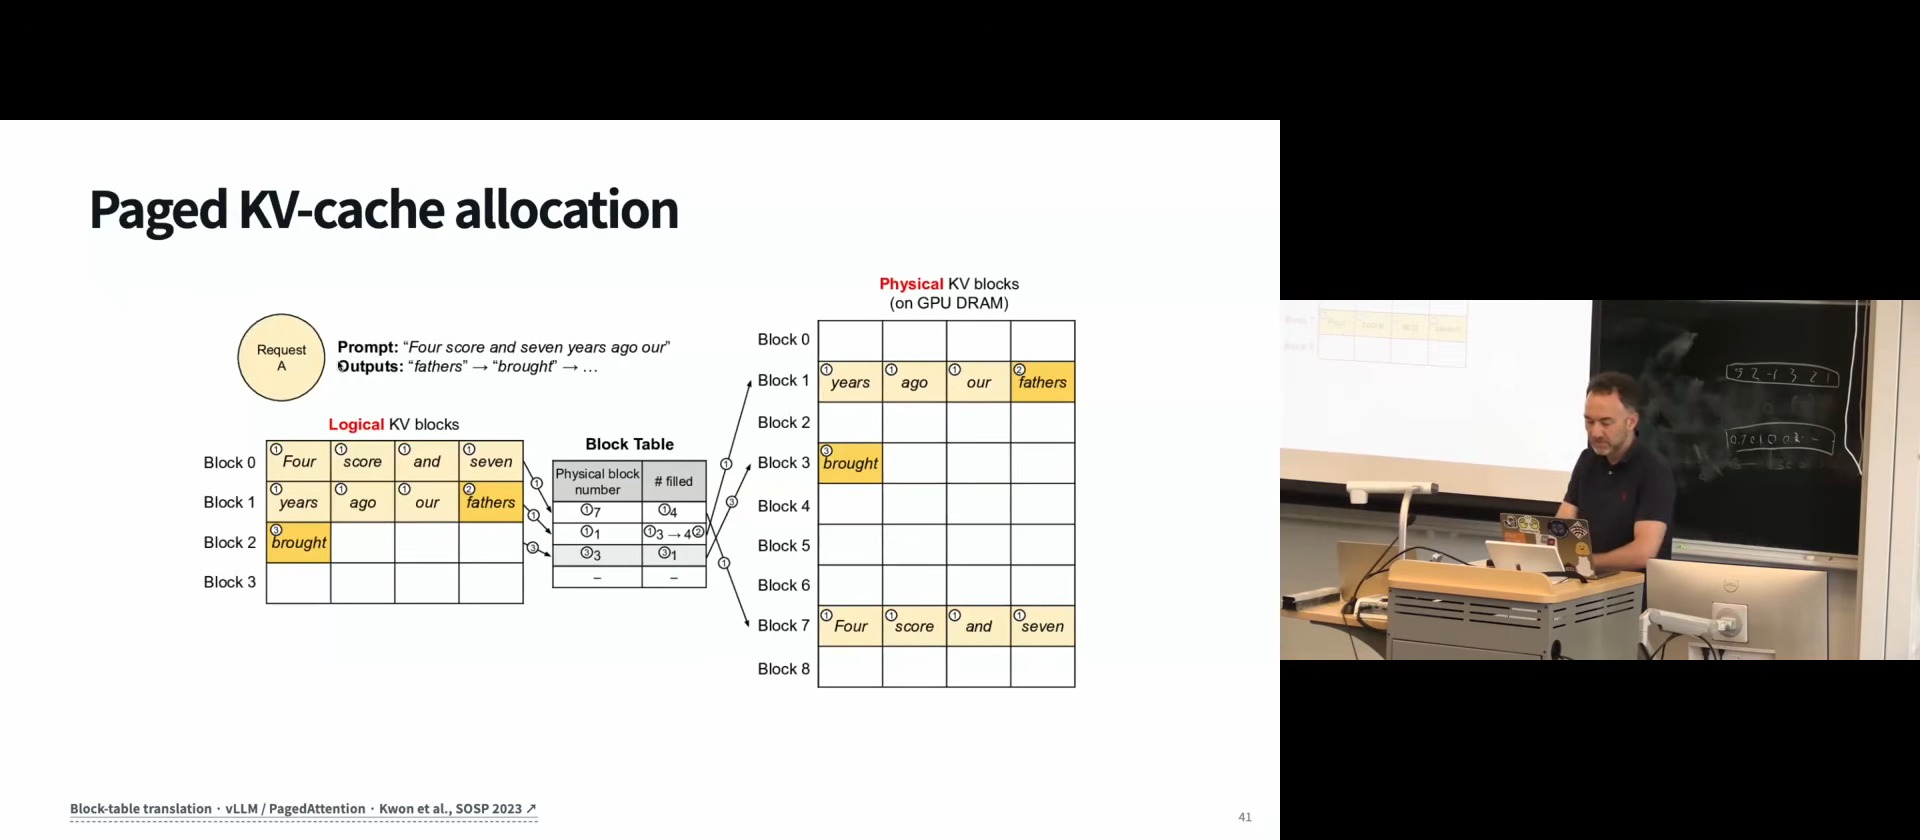
\includegraphics[width=\textwidth]{figures/fig_30_paged_attention.jpg}
\caption{Paged KV-cache：物理块、逻辑块与 block table 的地址翻译，支持按块分配与驱逐\vtag}
\end{figure}
\srcnote{00:58:30--00:58:44}

\subsection{RadixAttention：用前缀树找可以复用的开头}

SGLang 的 RadixAttention 用一棵基数树（radix tree）保存已经处理过的前缀。新请求到来时先沿树匹配公共前缀，命中的部分直接复用，只需为新后缀计算；请求结束后按 LRU 驱逐叶子节点。

\begin{figure}[H]
\centering
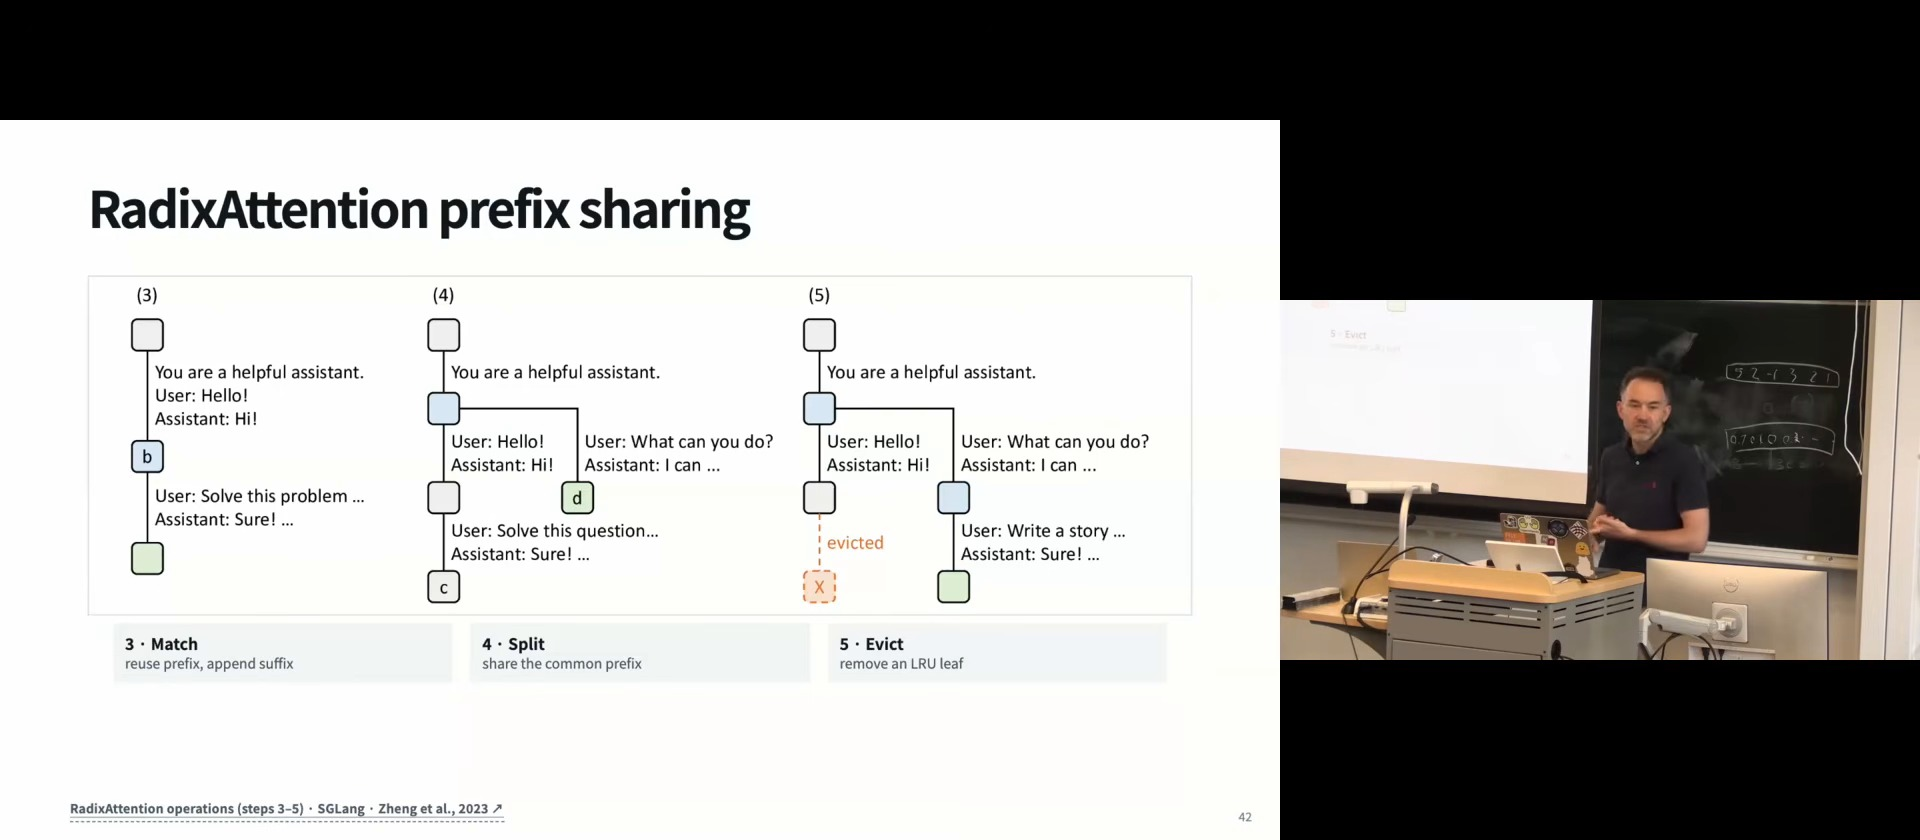
\includegraphics[width=\textwidth]{figures/fig_31_radix_attention.jpg}
\caption{RadixAttention：基数树匹配公共前缀，命中后复用、追加后缀，LRU 驱逐叶子\vtag}
\end{figure}
\srcnote{00:59:15--00:59:29}

这套结构最初是为聊天机器人设计的（多轮对话天然共享前缀），但对 agent 更重要，因为 agent 的历史更长、请求更频繁。除了单机内的复用，多机部署还要做\textbf{缓存感知路由}：请求进来时按“可复用前缀长度减去队列惩罚”选择 worker，把请求送到缓存最匹配的那台机器上。

\begin{figure}[H]
\centering
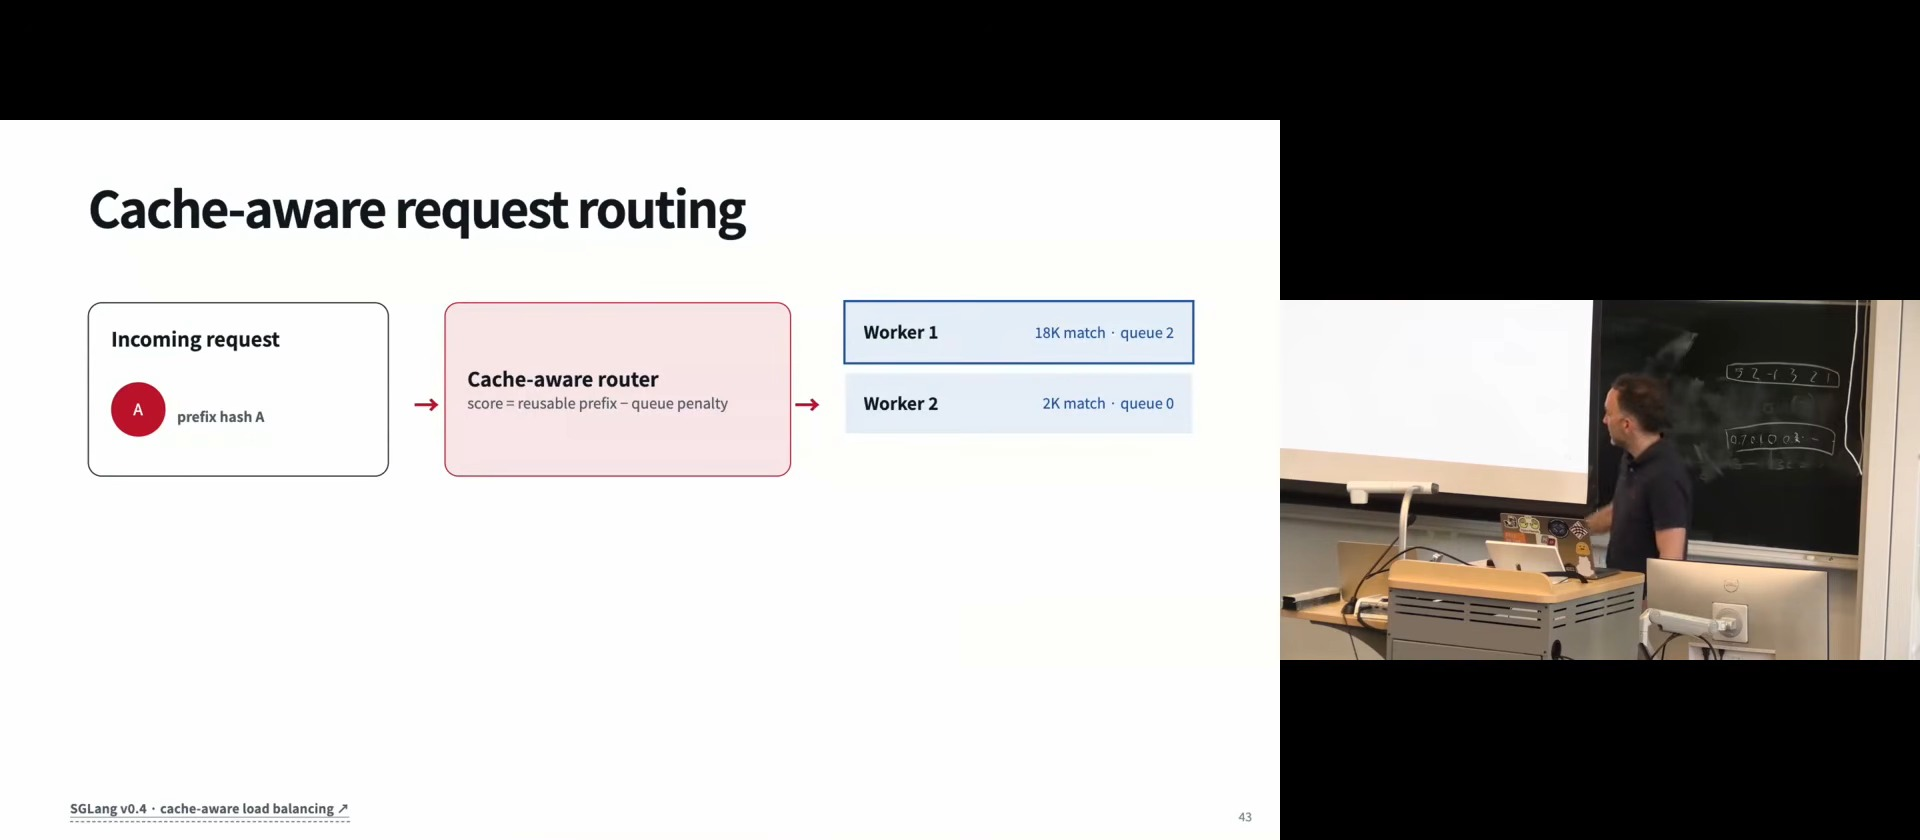
\includegraphics[width=\textwidth]{figures/fig_32_cache_routing.jpg}
\caption{缓存感知路由：router 按可复用前缀长度减队列惩罚选择 worker（18K match 对 2K match）\vtag}
\end{figure}
\srcnote{00:59:45--00:59:59}

讲者用 OpenRouter 的供应商数据说明这些工程差异会直接暴露在指标上：同一个模型，不同供应商的缓存命中率可以从 2.2\% 到 95.0\% 不等，最慢的一家（讲者点名 Mistral）命中率最差。他同时提醒这不能完全归咎于供应商水平，也可能反映各家承载的工作负载不同；但缓存路由与驱逐速度确实是可优化项。

\begin{figure}[H]
\centering
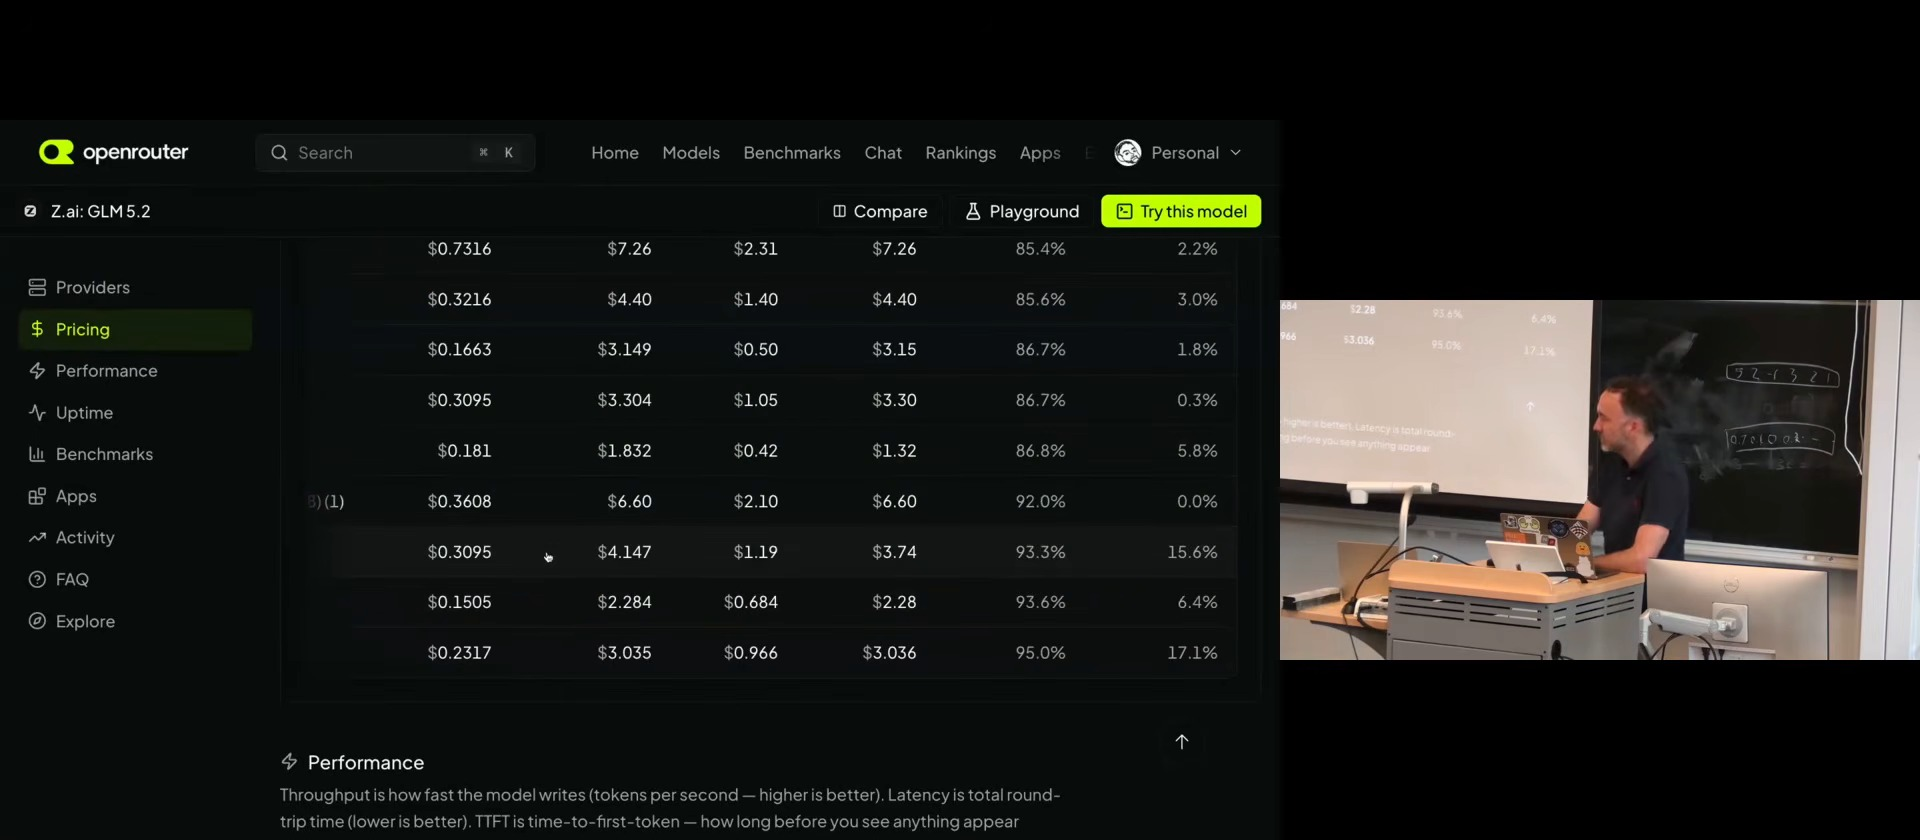
\includegraphics[width=\textwidth]{figures/fig_33_cache_hit_ranking.jpg}
\caption{同一模型各供应商的缓存命中率：从 2.2\% 到 95.0\%，差异直接进入账单\vtag}
\end{figure}
\srcnote{00:61:00--00:61:14}

\begin{knowledgebox}{缓存会过期，而且不会给你打折}
供应商不会无限期保存前缀：讲者记得 Anthropic 早年只有 5 分钟，现在可以选到 1 小时，但可能需要额外付费；过期后窗口被驱逐，下一次请求就要重新 prefill。对使用者不利的一点是单价不随命中率变化——同样按 token 收费，命中失败的部分等于白付。多机集群可能有 64 或 128 个节点，节点间路由与驱逐策略因此直接决定实际成本。
\end{knowledgebox}

\subsection{harness 纪律：不要悄悄打破前缀}

对写 harness 的人来说，缓存能否命中取决于一个非常严格的条件：\textbf{前缀必须逐字节一致}。因此讲者列出了一组“看起来合理但完全禁止”的做法。

\begin{lstlisting}[language=Python, caption=缓存友好的消息拼装（按讲者的三条纪律改写）]
def build_request(stable_system_prompt, stable_tools, history,
                  user_text, now_iso):
    # 1) prefix: system prompt + tool schema, byte-identical every step
    prefix = serialize(stable_system_prompt) + serialize(stable_tools)

    # 2) volatile state is appended to the LAST message, never to the prefix
    tail = user_text + "\n\n[current time: " + now_iso + "]"

    # 3) unchanged prefix -> provider can reuse its KV / page cache
    return prefix + history + [tail]
\end{lstlisting}

第一，\textbf{不要每一步都改 system message}。把当前时间日期写进 system prompt 是最常见的错误：时间每步都变，前缀每步都不同，等于完全没有缓存。需要时间就追加到最后一条用户消息或最近一条工具结果里。第二，\textbf{中途换工具是允许的}，改的是后缀而不是前缀。第三，\textbf{不要每一步切到不同模型}：换到别的模型意味着重新 prefill，而且回到贵模型时它之前的缓存已经不在，等于为高价 token 付两次钱。讲者说，只有当切换节省的费用能盖过重新 prefill 的成本时才值得做。

\begin{figure}[H]
\centering
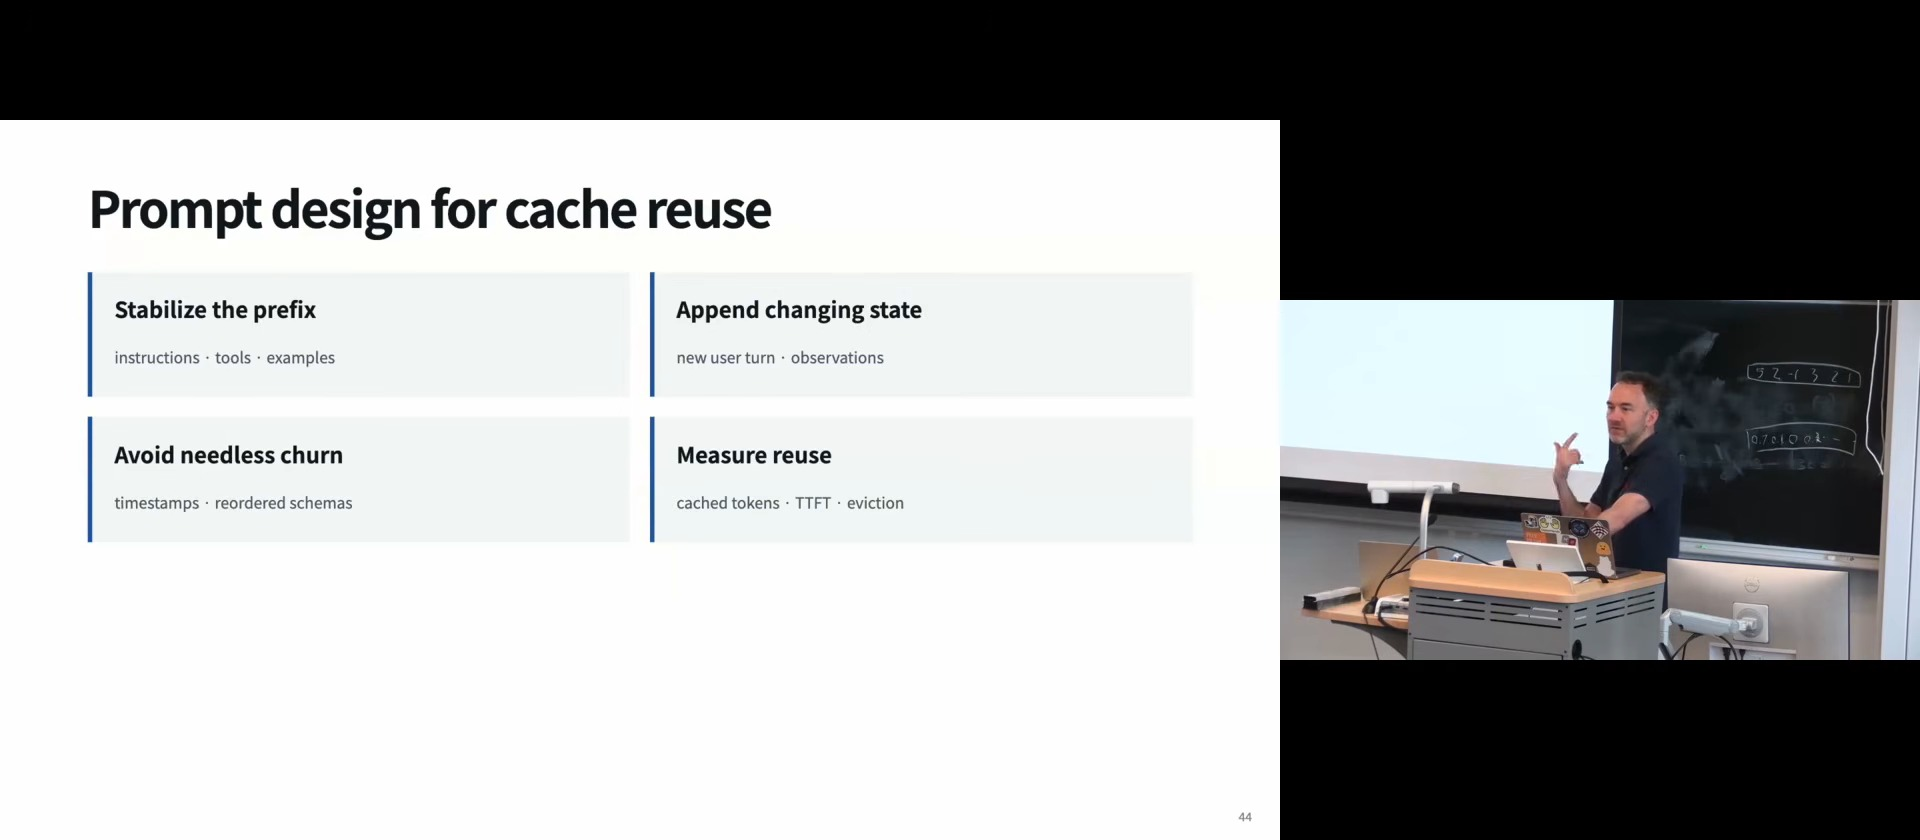
\includegraphics[width=\textwidth]{figures/fig_34_prompt_design.jpg}
\caption{缓存友好的提示设计：稳定前缀、变化状态只追加尾部、度量复用、避免时间戳等扰动\vtag}
\end{figure}
\srcnote{00:65:00--00:65:14}

\begin{warningbox}{三个最常见的“缓存杀手”}
（1）把时间、日期、运行编号写进 system prompt；（2）每一步重新序列化工具定义，字段顺序或空白发生变化；（3）为省钱频繁切换模型或供应商。它们的共同特征是“只改变了前缀的一小部分”，但缓存要求的是整段前缀一致，一处不同就全部失效。
\end{warningbox}

\subsection{本章小结}
服务端用 PagedAttention 的块表与 RadixAttention 的前缀树管理 KV 复用，多机还要按可复用前缀做路由，供应商之间的命中率可以差到 2.2\% 与 95.0\%；harness 侧则必须守住“前缀逐字节稳定”这条纪律，把变化的状态放在尾部、避免频繁换模型。缓存解决的是“不要重算已经算过的”，但它并不减少可见的历史长度——当历史真的长到无法承受时，就要动最后的工具：压缩。

\section{上下文压缩（compaction）}

\subsection*{本节回答的问题}
压缩到底删掉了什么、保留了什么？什么时候触发、用什么方式替换？为什么一个在基准上不掉分的压缩策略，到了真实使用里会让 agent 行为失常？

\subsection{一个具体例子}

幻灯片给了一个最小可懂的压缩场景：目标是把超时的 CI 修好。压缩前，历史里塞着一条 24K 行的日志，里面反复出现“address already in use”；压缩后只留下四样东西——原因（端口冲突）、做过并验证过的动作（改为 \texttt{--workers=1} 后通过）、证据的位置（\texttt{/tmp/ci.log}），以及下一步（提交 PR）。

\begin{figure}[H]
\centering
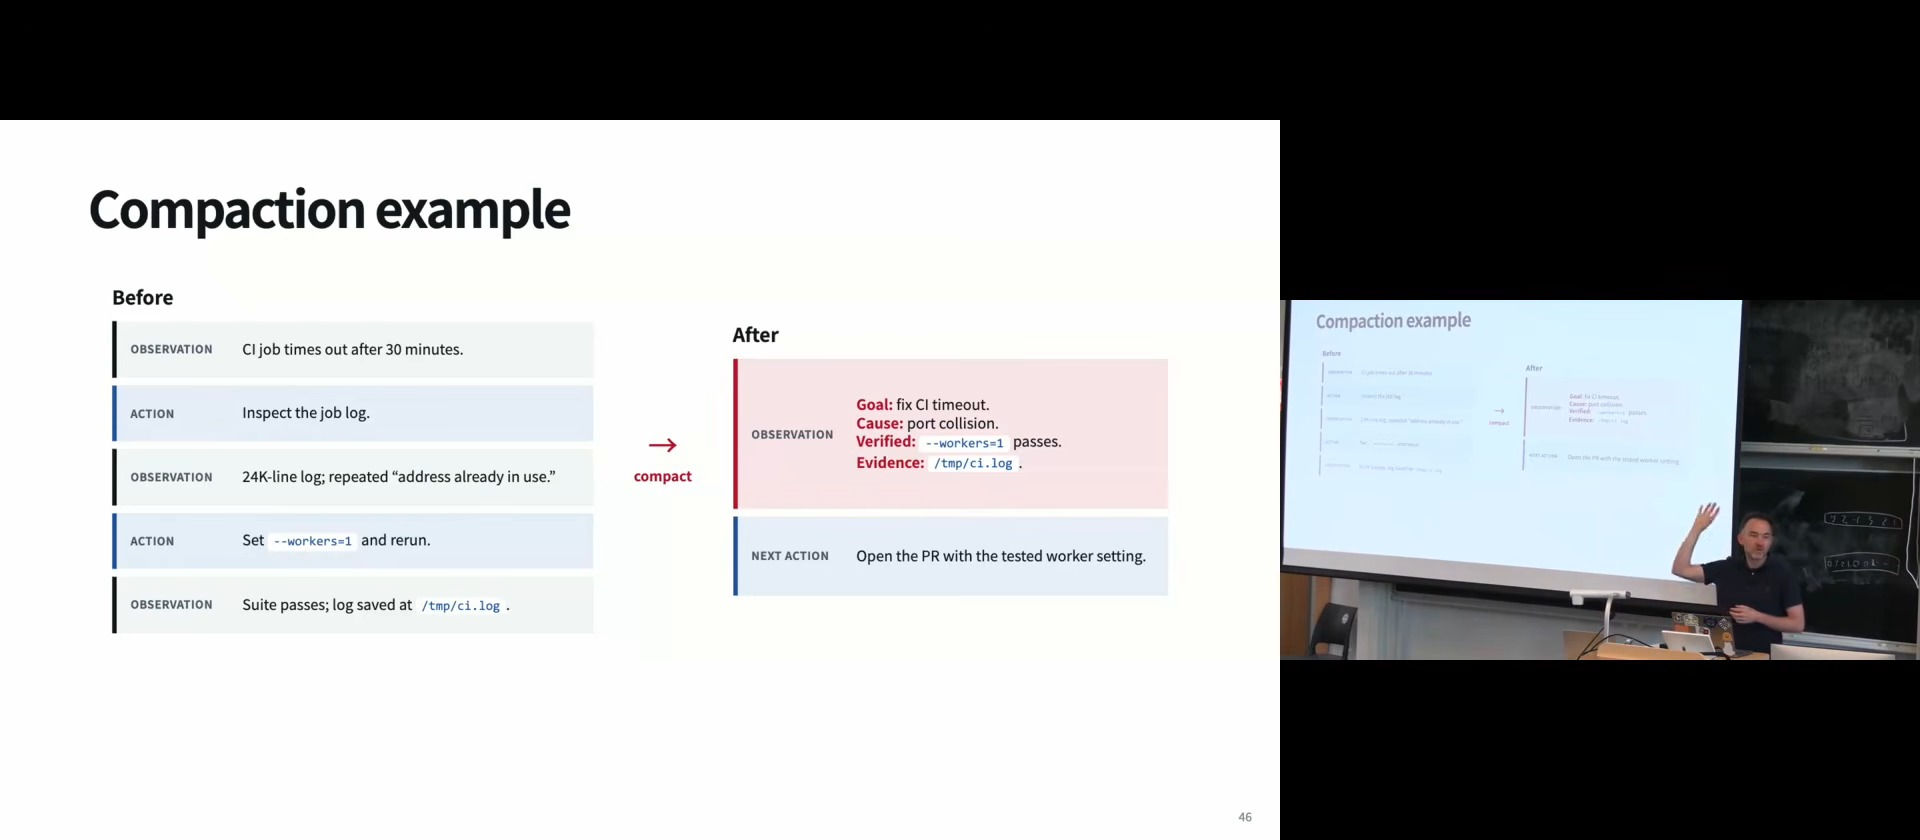
\includegraphics[width=\textwidth]{figures/fig_35_compaction_example.jpg}
\caption{压缩示例：把 24K 行日志压成原因、验证过的命令、证据路径与下一步动作\vtag}
\end{figure}
\srcnote{00:67:15--00:67:29}

压缩的价值在这里很直观：日志里 99\% 的内容对后续动作没有影响，但“端口冲突”这个结论、“已验证”这个状态和证据路径必须留下。压缩的错误方式是把日志截断成前若干行，那样既丢结论又留噪声。

\subsection{压缩是一种状态估计}

讲者给出一个更准确的形式化：压缩器 $C$ 把完整历史 $H_t$ 映射成有预算 $B$ 的工作状态 $s_t$。

\[
s_t=C(H_t,B),\qquad
|s_t|\le B,\qquad
p\!\left(A_{\text{future}}\mid H_t\right)\approx p\!\left(A_{\text{future}}\mid s_t\right)
\]

\begin{itemize}
\item $H_t$：到时刻 $t$ 的完整历史；$s_t$：压缩后的工作状态；$B$：状态允许的 token 预算；
\item 第一条约束“表示有界”要求 $s_t$ 不超过预算；
\item 第二个近似“行为保真”要求基于 $s_t$ 的未来动作分布与基于完整历史时接近；
\item 与之并列的第三个要求“可恢复”：精确锚点要原样保留，并留下指回原始证据的指针。
\end{itemize}

\begin{figure}[H]
\centering
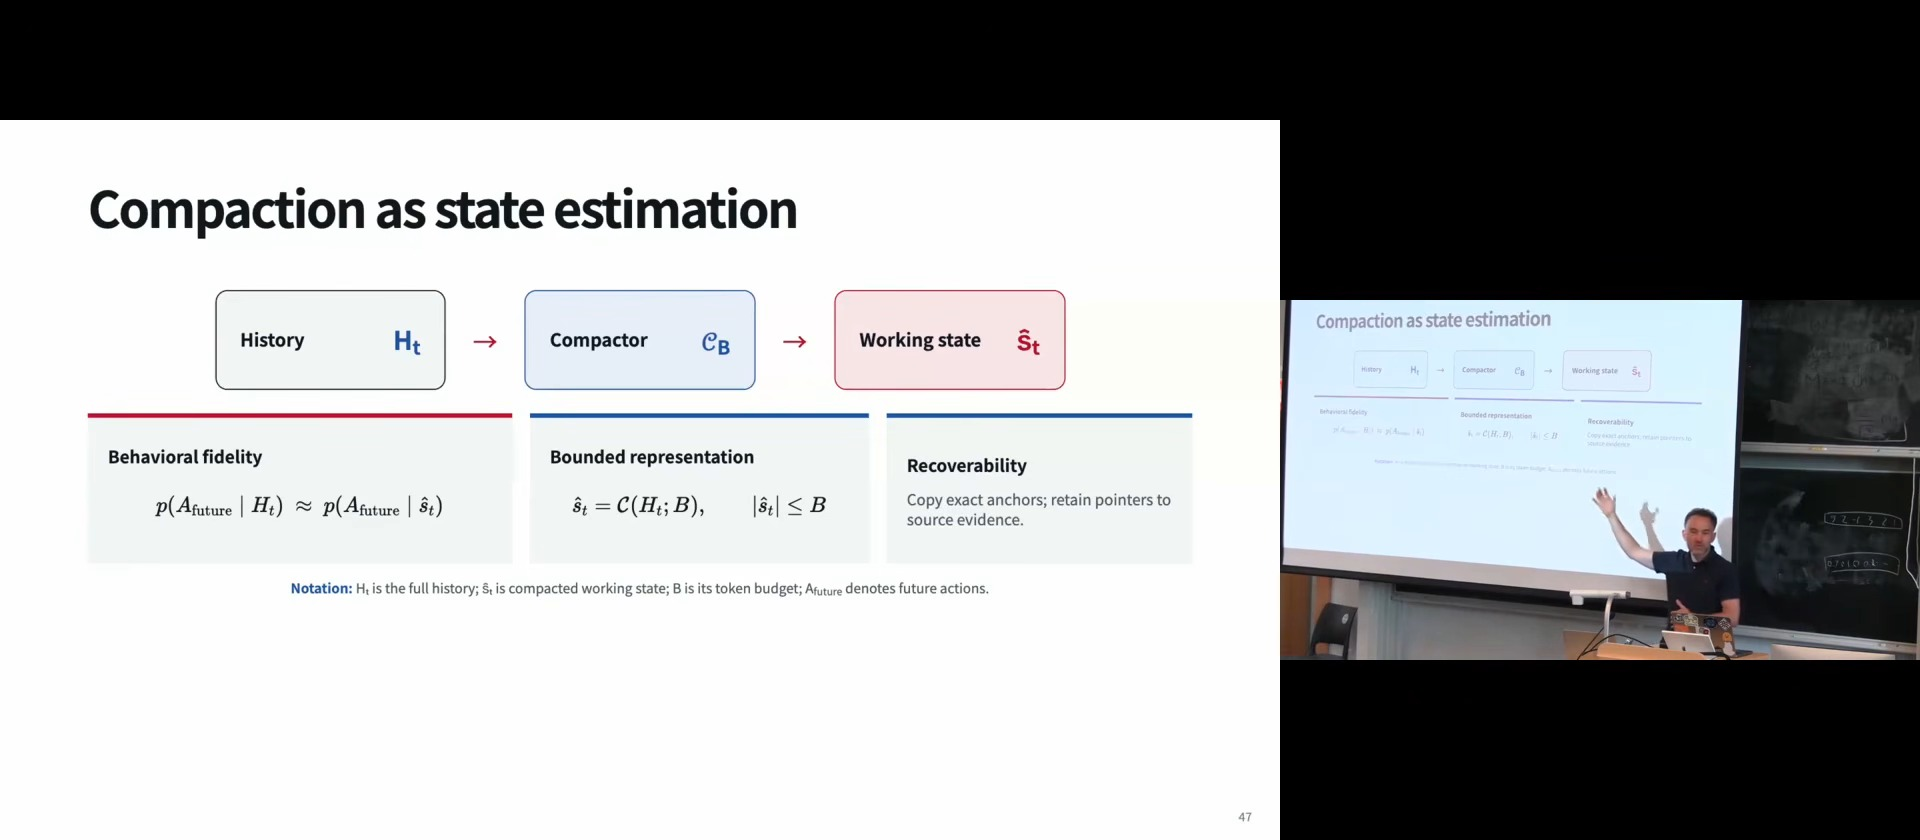
\includegraphics[width=\textwidth]{figures/fig_36_compaction_state.jpg}
\caption{压缩作为状态估计：$s_t=C(H_t,B)$，要求行为保真、表示有界与可恢复\vtag}
\end{figure}
\srcnote{00:67:45--00:67:59}

这个形式化解释了两类常见误解。把压缩当成“摘要”只满足表示有界，不保证行为保真；把压缩当成“截断”连可恢复性也丢掉了，因为被丢的内容既不在状态里也没有指针。

\subsection{压缩中保留什么}

幻灯片把模型可见的上下文分成三类处理。\textbf{精确保留}的是锚点（目标与约束）与最近的尾部（当前尝试与最新结果）；\textbf{编码}的是中段，把决策与进展压成 checkpoint；\textbf{外置}的是证据，把大日志变成“3 个失败点 + 命令 + 产物路径”放进 evidence store，需要时再取回；剩下的重复内容与被取代的尝试直接丢弃。

\begin{figure}[H]
\centering
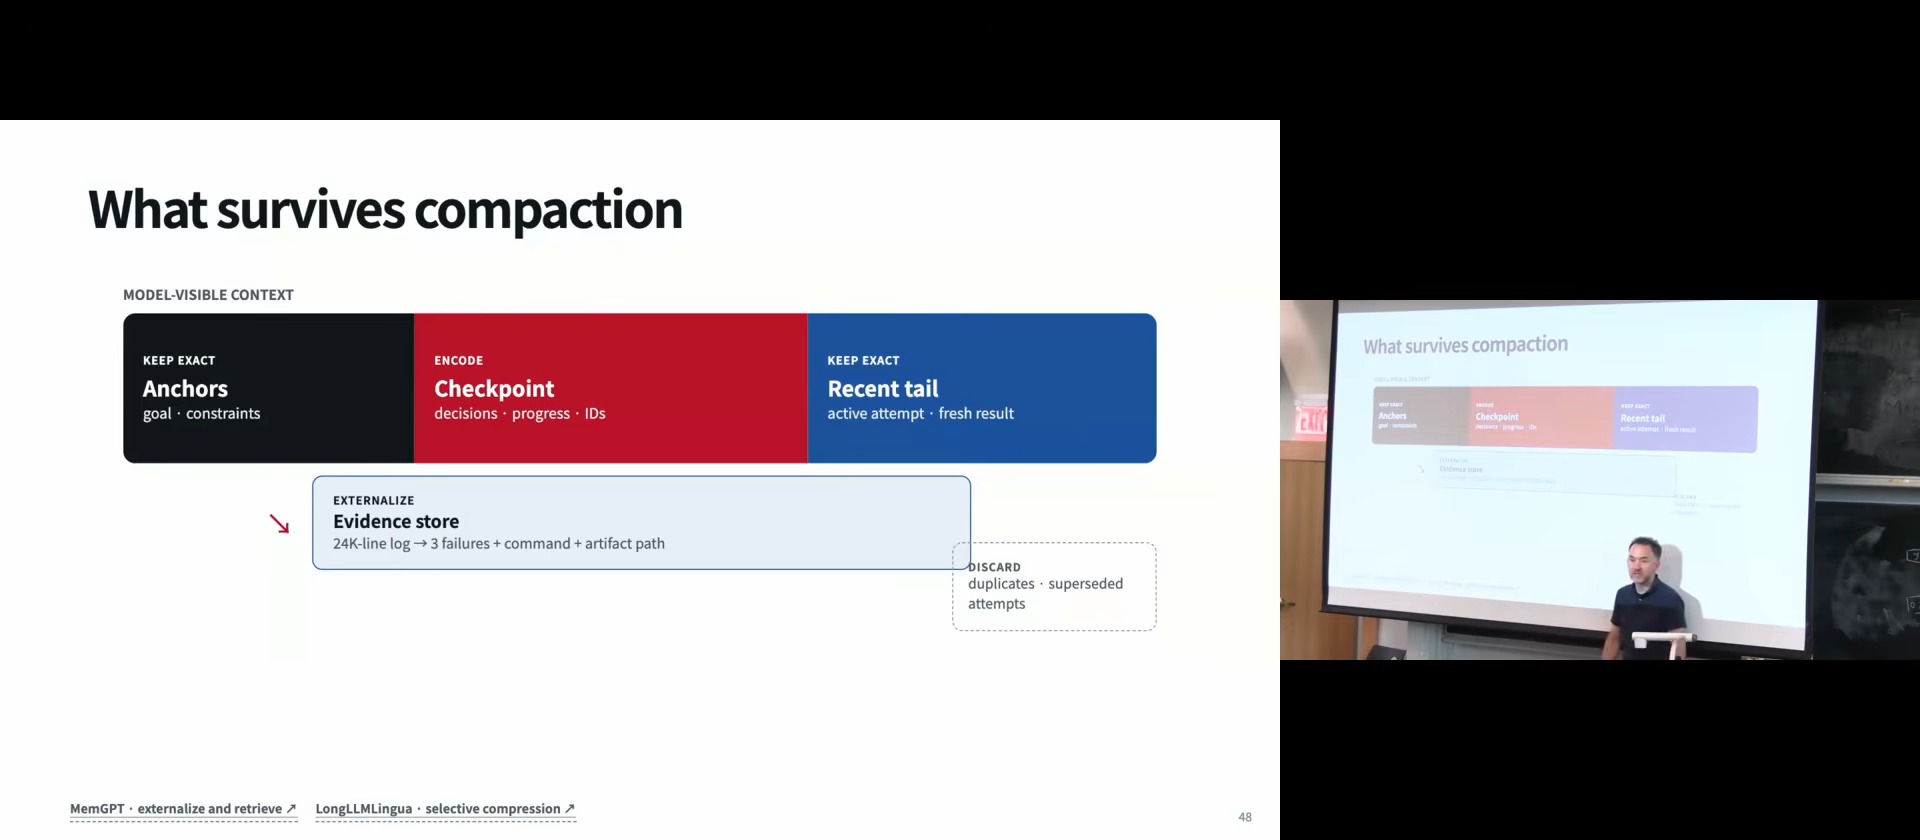
\includegraphics[width=\textwidth]{figures/fig_37_what_survives.jpg}
\caption{压缩中保留什么：锚点与最近尾部精确保留，中段编码为 checkpoint，证据外置到 evidence store\vtag}
\end{figure}
\srcnote{00:68:45--00:68:59}

讲者特别强调“保护开头”：会话最开始的目标与约束往往最重要，而它恰恰最容易被通用摘要算法当成“陈旧内容”丢掉。他提到自己在课上问“agent 会忘掉什么”时，得到的回答之一正是“会话最开头的东西”——这有时是现有 harness 的设计缺陷，好的实现会刻意不删除开头。

\subsection{策略：触发、选择、替换}

压缩策略可以拆成三个决策。\textbf{触发}有三种：按 token 阈值（例如到 200K 就压缩）、按供应商的硬上限（被上下文溢出逼着压）、或按用户手动请求（编码工具里的 \texttt{/compact}）。\textbf{选择}决定保护哪一段：保护开头、压缩较老的中段、保留最近尾部，并在完整的轮次或工具调用边界上切分。\textbf{替换}决定用什么形式承载中段：可读的自由文本摘要、要求特定字段的结构化 checkpoint（通过一次工具调用产出），或者供应商提供的不可读不透明条目。

\begin{figure}[H]
\centering
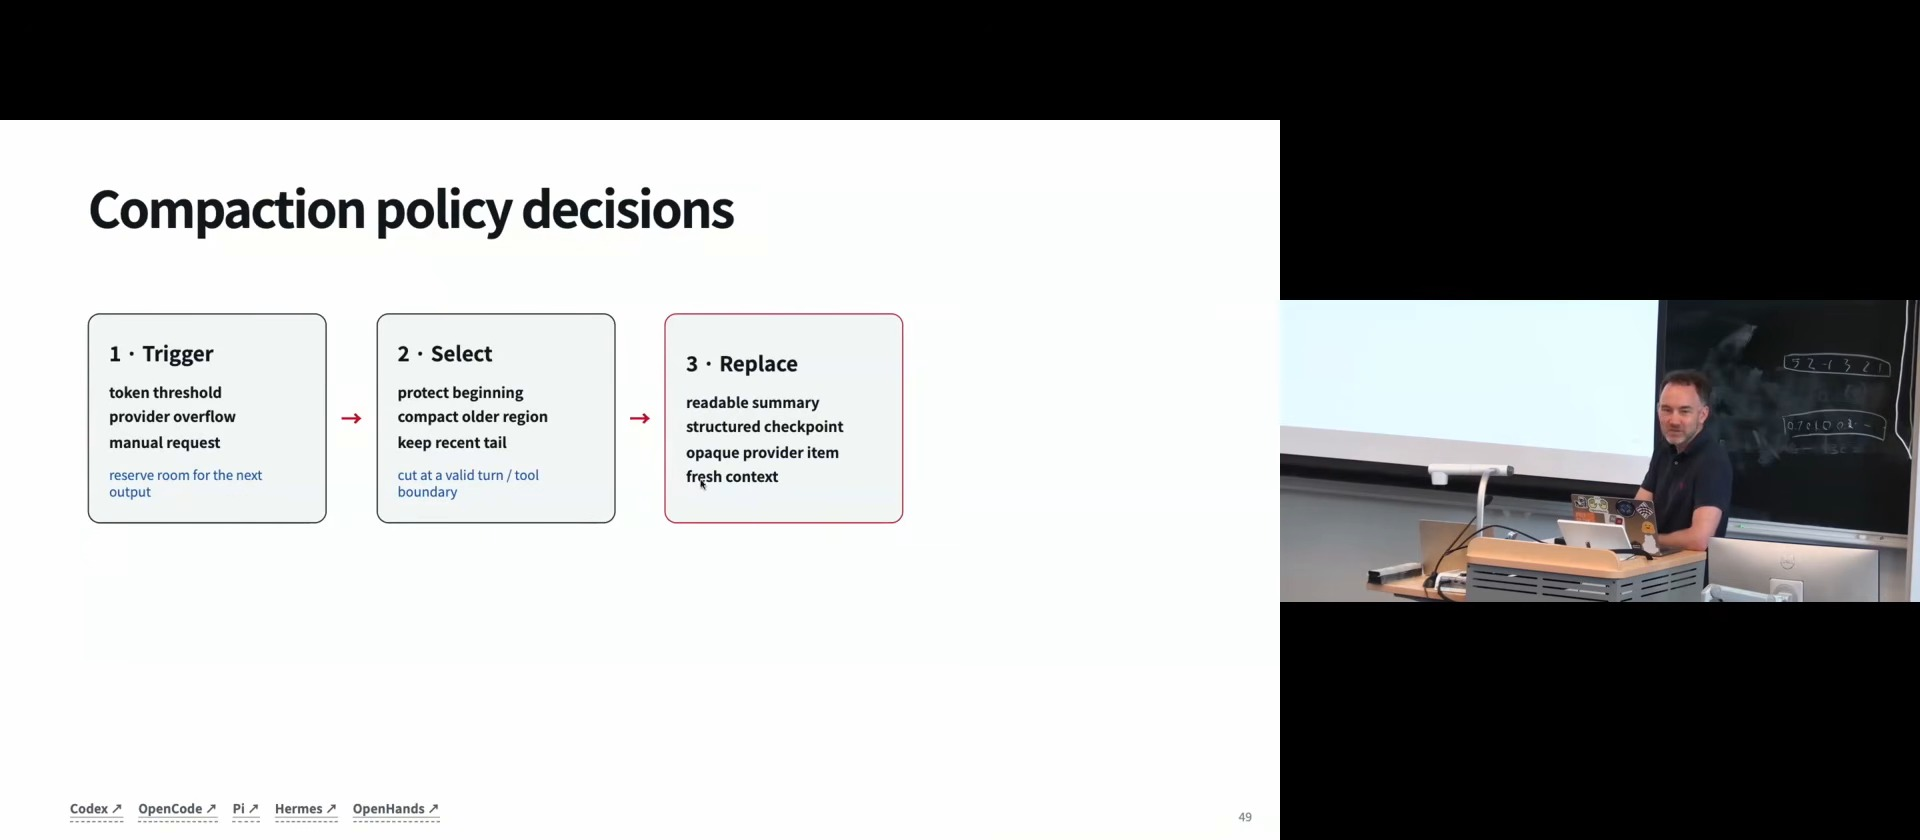
\includegraphics[width=\textwidth]{figures/fig_38_compaction_policy.jpg}
\caption{压缩策略三要素：触发（阈值/溢出/手动）、选择（保护开头、压缩中段、保留尾部）、替换方式\vtag}
\end{figure}
\srcnote{00:71:30--00:71:44}

讲者提到常见的三种替换形态：自由文本摘要最通用；结构化 checkpoint 要求压缩必须回答“目标、决策、进度、标识符”等固定字段，可审计性更好；有的厂商（讲者认为主要是 OpenAI）把压缩结果加密成不可读的内容，你看不到它删了什么。无论哪种，替换都应该在语义边界上发生，而不是把一个工具结果从中间切断。

\subsection{反复压缩的漂移与评测}

压缩不是一次性动作。会话继续，新的历史 $R_k$ 又会加进来，下一次压缩是在“上一份摘要”的基础上再做一次：

\[
S_{k+1}=C\left(S_k\oplus R_k\right)
\]

\begin{itemize}
\item $S_k$：第 $k$ 次压缩后的工作状态；$R_k$：其后新增的历史；
\item $\oplus$：把新增历史追加到已有状态上；
\item 每一次更新都继承上一次的近似，误差会累积，因此“压一次没问题”不代表“压十次没问题”。
\end{itemize}

\begin{figure}[H]
\centering
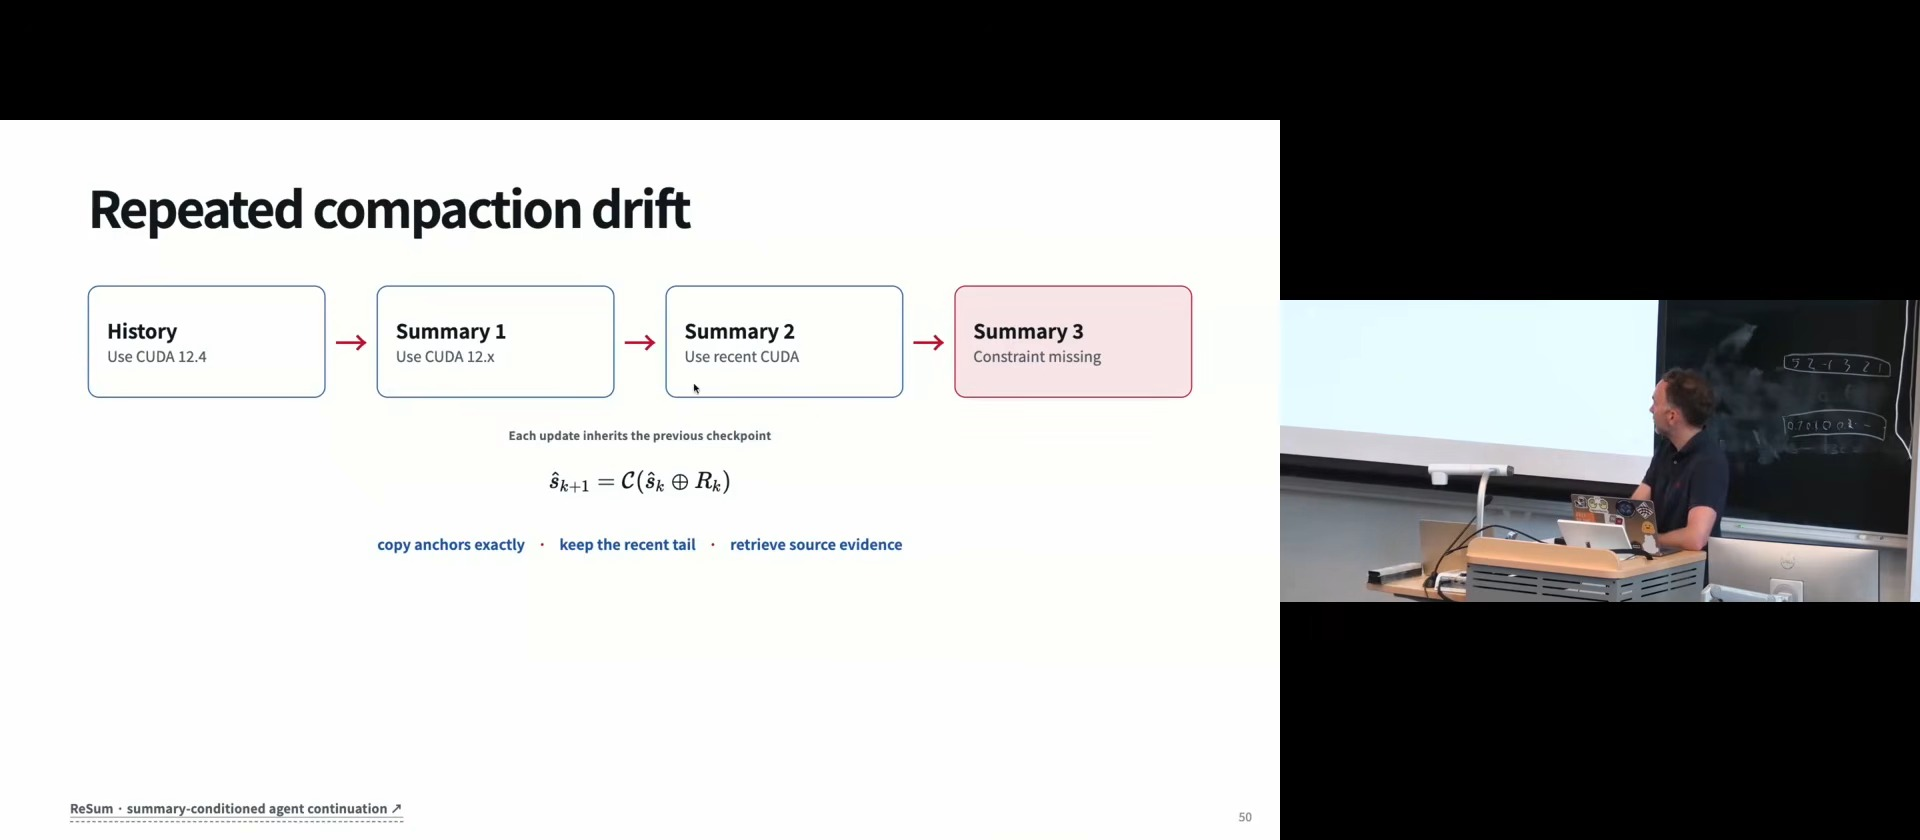
\includegraphics[width=\textwidth]{figures/fig_39_repeated_drift.jpg}
\caption{反复压缩的漂移：每次更新都继承上一份 checkpoint，约束可能在多轮压缩中遗失\vtag}
\end{figure}
\srcnote{00:72:00--00:72:14}

评测压缩不能只看最终任务成功率。幻灯片给出“基于续跑”的评测：先植入一段状态（约束、决策、产物），用生产策略压缩，再让 agent 继续；随后分别测状态召回（约束与标识符是否还在）、任务成功（续跑是否正确）、效率（token、延迟、成本）与稳定性（反复压缩后的表现）。

\begin{figure}[H]
\centering
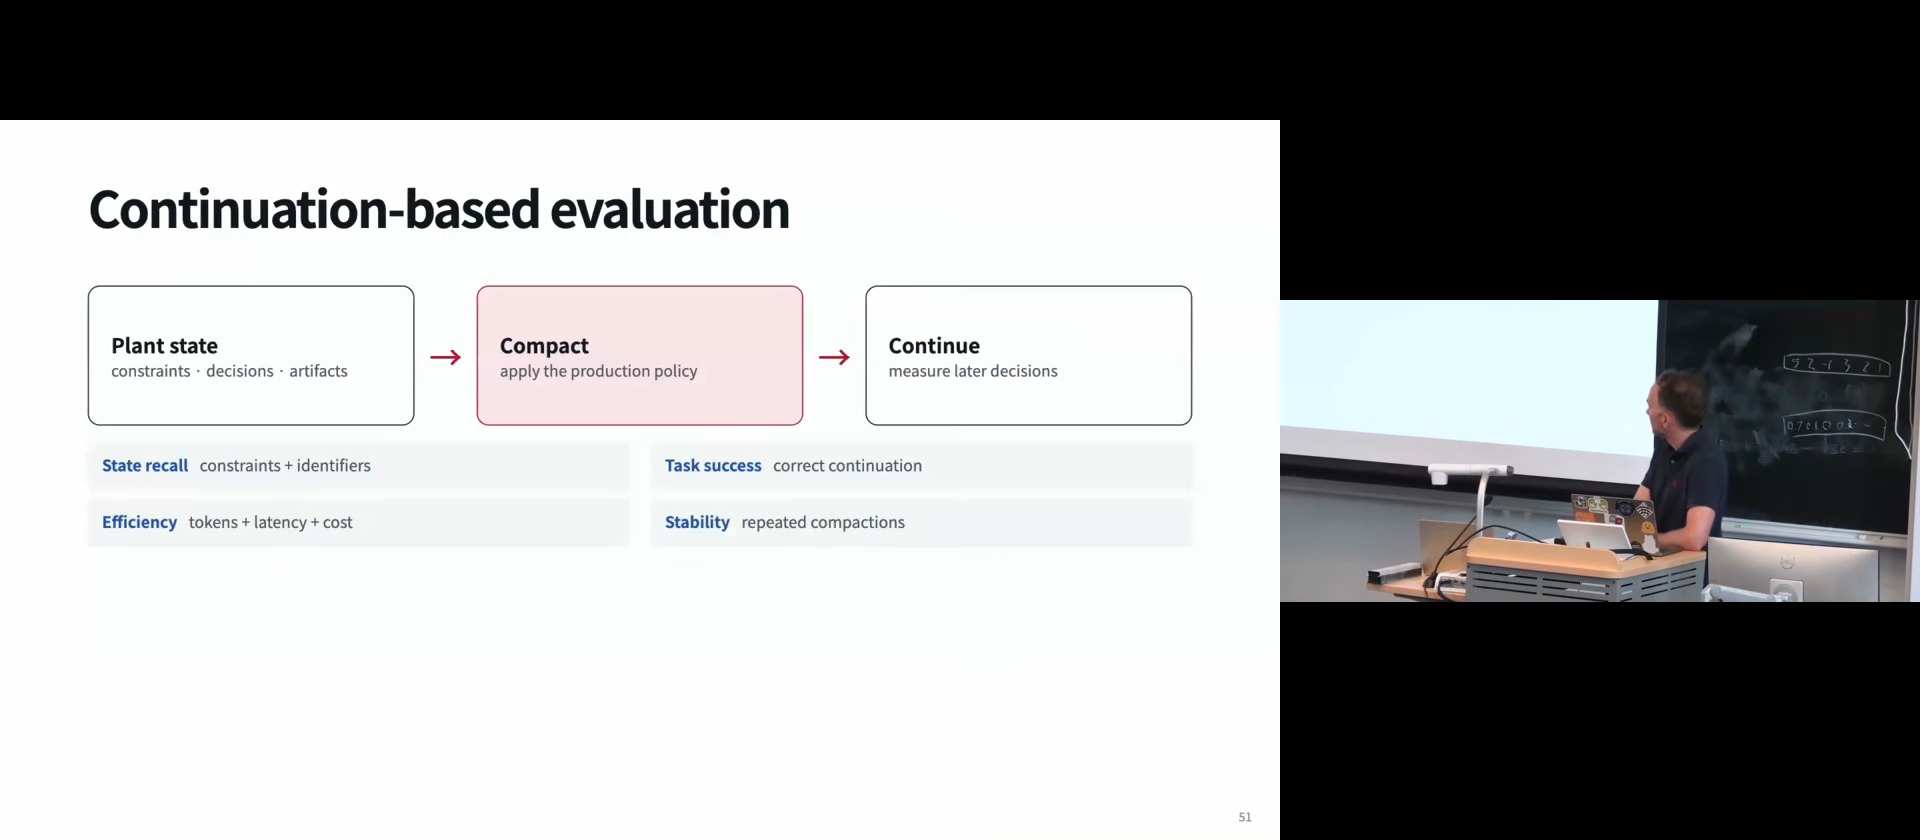
\includegraphics[width=\textwidth]{figures/fig_40_continuation_eval.jpg}
\caption{基于续跑的评测：压缩后测量状态召回、任务成功、效率与反复压缩的稳定性\vtag}
\end{figure}
\srcnote{00:72:15--00:72:29}

讲者讲了一个亲历的教训：OpenHands 早期做过一版他们认为生产可用的压缩策略，在当时常用的编码基准 SWE-bench 上完全不掉分，还省了大量 token；但放进真实系统后，agent 开始做很蠢的事——因为它忘了自己已经提交过 PR，同一功能连开了 5 个 PR；又因为基准只覆盖了“单个用户消息”的会话，它会把会话中途的用户指令压掉。结论是：只在单轮基准上验证压缩是不够的，必须有覆盖多轮交互的稳健基准，并且要在真实使用中测。

\begin{warningbox}{压缩的失败常常是“静默”的}
被丢掉的约束不会报错，模型会继续用剩下的信息自信地行动，直到做出违规操作——删文件、重复提交、忽略中途指令。因此压缩的验收标准不是“摘要读起来像”，而是“续跑行为一致”。凡是涉及不可逆动作（删除、发布、付费）的 agent，压缩前后都应保留显式约束并要求重新确认。
\end{warningbox}

\subsection{本章小结}
压缩把完整历史映成有预算的工作状态，必须以行为保真、表示有界、可恢复三条标准衡量；做法上是保护开头与最近尾部、把中段编码成 checkpoint、把证据外置成可按需取回的形式；策略由触发、选择、替换三个决策组成。反复压缩会累积漂移，评测必须看续跑行为而不只是摘要质量。最后回到整条链路，看这五层如何分工。

\section{总结与延伸}

\subsection*{本节回答的问题}
把这一讲的全部机制放在一张图里，它们各自负责什么、在哪里交接？

\subsection{讲者的收束}

讲者用一张“长上下文系统栈”收尾：agent loop 会不断把指令、动作与环境观察塞进上下文（Growth）；prefill、decode、稠密注意力与 KV 内存制造了不同的瓶颈（Inference）；局部、循环、稀疏与压缩机制决定历史中哪些部分仍然可达（Architecture）；稳定的前缀避免重复 prefill，但并不减少可见历史的长度（Caching）；压缩负责在超出预算时保留意图、精确任务状态、最近工作与恢复路径，并且要用续跑来验证（Compaction）。

\begin{figure}[H]
\centering
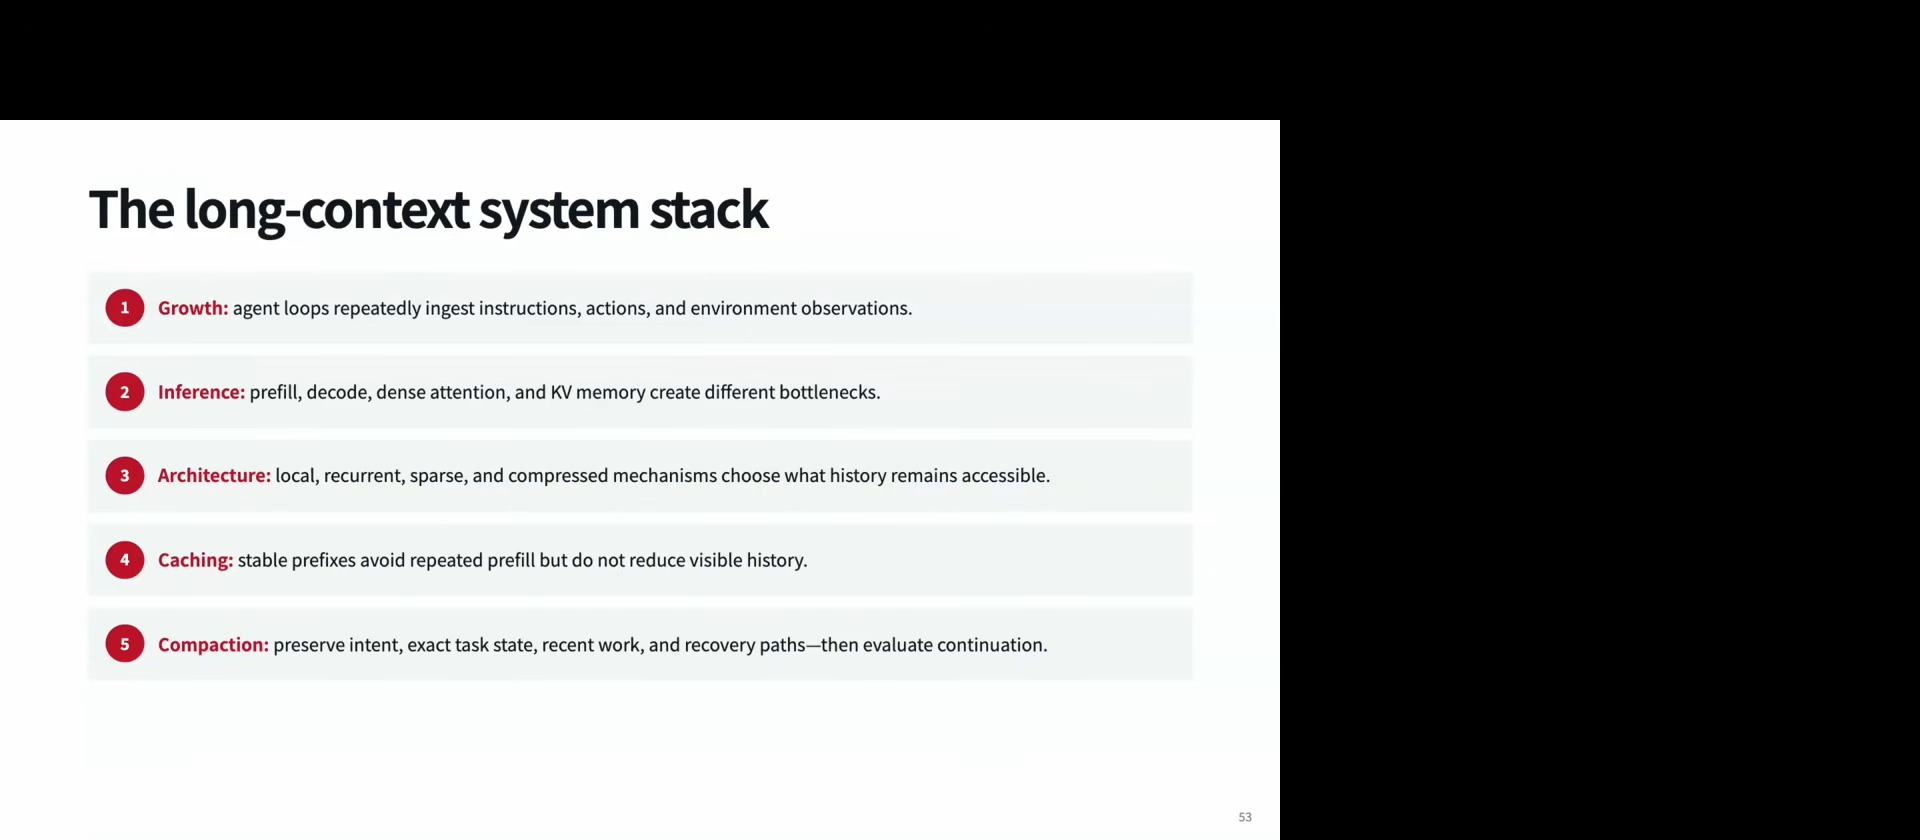
\includegraphics[width=\textwidth]{figures/fig_41_system_stack.jpg}
\caption{长上下文系统栈：Growth、Inference、Architecture、Caching、Compaction 五层各司其职\vtag}
\end{figure}
\srcnote{00:75:00--00:75:14}

\subsection{整理者的综合}

把这一讲压缩成一句判断：\textbf{长上下文不是单一技术，而是一条从注意力实现一直贯穿到提示拼装的流水线}。每一层解决的是不同的问题，换层不能替代。架构层把每个查询必须比较的位置数封顶，把历史压进固定大小的状态，或用稀疏与压缩减少要保存的键值，从而让百万级序列“算得起”；训练层用位置编码、长度课程与配套数据让模型“用得动”这些位置；缓存层让已经算过的前缀只算一次，把重复的二次成本拉回线性；压缩层在预算耗尽时做出取舍，决定哪些历史继续对模型可见。

四层之间的交接点也值得记住：缓存只对“逐字节相同的前缀”生效，所以 harness 的拼装顺序属于性能设计而不是代码风格；压缩会改变可见历史，因此必须与缓存协同——压缩后的新前缀当然无法命中旧缓存，这正是压缩要尽量稀疏触发、并按语义边界执行的原因；上下文并行与新的状态更新机制相互制约，说明模型架构的选择同时也是服务与训练工程的选择。

最后是可操作的检查清单：新会话开始前固定 system prompt 与工具定义；把时间、运行编号这类易变状态放在最后一条消息里；把缓存命中率、TTFT 与驱逐情况作为常规指标；对任何压缩策略，先在多轮交互的基准上验证，再在真实使用中观察它有没有丢失中途指令与已完成动作。

\subsection{可以继续追问的问题}

\begin{itemize}
\item 本讲没有展开 subagent 作为上下文管理手段的作用；讲者在问答里明确说“subagent 是，但我们留到后面讲”（对应下一讲 skills and memory）。
\item 缓存是否会分层（GPU 显存到 CPU 内存再到磁盘）？课堂上有人问，讲者坦承自己不知道答案，并说这是一个值得做的后续实验。
\item 内容相关稀疏注意力的选择器用什么相似度、是否需要归一化，讲者回答“通常是点积”，细节留在论文里。
\item 如何为上下文并行实现非标准状态更新（如 Gated Delta Net）的 kernel，是模型与系统团队之间的长期摩擦点，讲者以自己的经历说明它经常决定一个想法能否落地。
\end{itemize}

\subsection{拓展阅读}
讲义提到的机制对应以下公开工作，供读者按图索骥：注意力原始论文（Vaswani 等，2017）、PagedAttention 与 vLLM（Kwon 等，SOSP 2023）、RadixAttention 与 SGLang、Ring Attention（Liu 等，2023）、位置插值（Chen 等，2023）、RoPE（Su 等，2024）、NoPE 的长度泛化分析（Kazemnejad 等，NeurIPS 2023）、YaRN（Peng 等，ICLR 2024）、Gated Delta Networks（Yang 等，2024）、Kimi Linear/KDA（Kimi 团队，2025）、GQA（Ainslie 等，2023）与 MLA（DeepSeek-V2，2024）。这些内容以幻灯片标注为准，本讲义未引入幻灯片之外的结论。

\end{document}
